\documentclass[10pt,twocolumn]{article}
\usepackage[T1]{fontenc}
\usepackage{lmodern}
\usepackage[margin=0.75in]{geometry}
\usepackage{booktabs}
\usepackage{amsmath,amssymb}
\usepackage{amsthm}  % proof environment + \newtheorem styling (identifiability theorem section)
\usepackage{graphicx}
\usepackage{xcolor}
\usepackage{caption}
\usepackage[numbers,sort&compress]{natbib}
\usepackage[hidelinks]{hyperref}
\hypersetup{pdftitle={What a Verifiable Reward Can and Cannot Credit in Self-Extending
  Agent Memory: A Non-Identifiability Result for False-Lesson Harm},
  pdfauthor={James Hugglestone, Samuel Jacob Chacko, Xiuwen Liu}}
\usepackage{microtype}
\captionsetup{font=small,labelfont=bf}
\graphicspath{{./}}

% --- result macros: providecommand fallbacks so the paper compiles before the
%     experiment finishes; numbers.tex (emitted by experiments/analyze.py from the
%     logs) overrides each one, so every number in the prose traces to a log. ---
\providecommand{\BzeroSolve}{[B0]}
\providecommand{\BtwoSolve}{[B2]}
\providecommand{\BtwoLift}{[lift]}
\providecommand{\BtwoCIlo}{[lo]}\providecommand{\BtwoCIhi}{[hi]}
\providecommand{\Npairs}{[n]}
\providecommand{\BfourSolve}{[B4]}
\providecommand{\BfourLiftBzero}{[d]}\providecommand{\BfourLiftBtwo}{[d]}
\providecommand{\Qtrue}{[Qt]}\providecommand{\Qpoison}{[Qp]}
\providecommand{\PoisonCite}{[pc]}
\providecommand{\QpoisonAllM}{[Qp]}\providecommand{\QpoisonOutcome}{[Qp]}
\providecommand{\LooPoison}{[lp]}\providecommand{\LooTrue}{[lt]}\providecommand{\Exposure}{[e]}
\providecommand{\OpeMeasured}{[m]}\providecommand{\OpeDR}{[dr]}\providecommand{\OpeBestTau}{[t]}
\providecommand{\QdistractCited}{[qd]}\providecommand{\QdistractAllM}{[qd]}
\providecommand{\QtrueAllM}{[qt]}\providecommand{\RecovMask}{[rm]}
\providecommand{\GatedProv}{[g]}\providecommand{\GatedTrust}{[g]}\providecommand{\GatedTotal}{[g]}
\providecommand{\GatedProvPct}{[g]}\providecommand{\UngatedTrust}{[u]}
\providecommand{\UngatedTotal}{[u]}\providecommand{\UngatedTrustPct}{[u]}
\providecommand{\NchalPairs}{[n]}\providecommand{\BtwoLiftChalP}{[p]}\providecommand{\SeedAgree}{[s]}
\providecommand{\NCeiling}{[c]}\providecommand{\NFloor}{[f]}\providecommand{\NLift}{[l]}
\IfFileExists{numbers.tex}{\providecommand{\BzeroSolve}{}\renewcommand{\BzeroSolve}{54\%}
\providecommand{\BtwoSolve}{}\renewcommand{\BtwoSolve}{66\%}
\providecommand{\BtwoLift}{}\renewcommand{\BtwoLift}{+0.12}
\providecommand{\BtwoCIlo}{}\renewcommand{\BtwoCIlo}{+0.05}
\providecommand{\BtwoCIhi}{}\renewcommand{\BtwoCIhi}{+0.21}
\providecommand{\Npairs}{}\renewcommand{\Npairs}{80}
\providecommand{\NchalPairs}{}\renewcommand{\NchalPairs}{40}
\providecommand{\BtwoLiftChalP}{}\renewcommand{\BtwoLiftChalP}{0.031}
\providecommand{\SeedAgree}{}\renewcommand{\SeedAgree}{37}
\providecommand{\NCeiling}{}\renewcommand{\NCeiling}{5}
\providecommand{\NFloor}{}\renewcommand{\NFloor}{2}
\providecommand{\NLift}{}\renewcommand{\NLift}{3}
\providecommand{\BfourSolve}{}\renewcommand{\BfourSolve}{61\%}
\providecommand{\BfourLiftBzero}{}\renewcommand{\BfourLiftBzero}{+0.07}
\providecommand{\BfourLiftBtwo}{}\renewcommand{\BfourLiftBtwo}{-0.05}
\providecommand{\Qtrue}{}\renewcommand{\Qtrue}{+0.34}
\providecommand{\Qpoison}{}\renewcommand{\Qpoison}{+0.40}
\providecommand{\PoisonCite}{}\renewcommand{\PoisonCite}{44\%}
\providecommand{\QdistractCited}{}\renewcommand{\QdistractCited}{+0.00}
\providecommand{\RecovMask}{}\renewcommand{\RecovMask}{69\%}
\providecommand{\QpoisonAllM}{}\renewcommand{\QpoisonAllM}{+0.29}
\providecommand{\QtrueAllM}{}\renewcommand{\QtrueAllM}{+0.29}
\providecommand{\QdistractAllM}{}\renewcommand{\QdistractAllM}{+0.36}
\providecommand{\QpoisonOutcome}{}\renewcommand{\QpoisonOutcome}{+0.40}
\providecommand{\GatedProv}{}\renewcommand{\GatedProv}{13}
\providecommand{\GatedTrust}{}\renewcommand{\GatedTrust}{5}
\providecommand{\GatedTotal}{}\renewcommand{\GatedTotal}{18}
\providecommand{\GatedProvPct}{}\renewcommand{\GatedProvPct}{72\%}
\providecommand{\UngatedTrust}{}\renewcommand{\UngatedTrust}{13}
\providecommand{\UngatedTotal}{}\renewcommand{\UngatedTotal}{19}
\providecommand{\UngatedTrustPct}{}\renewcommand{\UngatedTrustPct}{68\%}
\providecommand{\LooPoison}{}\renewcommand{\LooPoison}{+0.00}
\providecommand{\LooTrue}{}\renewcommand{\LooTrue}{+0.40}
\providecommand{\Exposure}{}\renewcommand{\Exposure}{90\%}
\providecommand{\OpeMeasured}{}\renewcommand{\OpeMeasured}{0.77}
\providecommand{\OpeDR}{}\renewcommand{\OpeDR}{0.77}
\providecommand{\OpeBestTau}{}\renewcommand{\OpeBestTau}{2.0}
}{}
% Solution-paper numbers: defaults first (define every macro), then the analyzer's
% computed values override on top (\renewcommand). Robust to partial campaigns.
\IfFileExists{numbers_solution_defaults.tex}{% STUB — overwritten by experiments/analyze_campaign.py once results/campaign_v2
% exists. Defines every macro results_solution.tex references so the paper compiles
% before the v2 run finishes. Placeholder value "\,?\," flags un-filled numbers.
\providecommand{\stubq}{\,?\,}
\providecommand{\CampNtrain}{\stubq}
\providecommand{\CampNheldout}{\stubq}
\providecommand{\CampEpochs}{\stubq}
\providecommand{\CampEvalSeeds}{\stubq}
\providecommand{\CampRerolls}{\stubq}
\providecommand{\CampBzero}{\stubq}
\providecommand{\CampBtwo}{\stubq}
\providecommand{\CampOutcome}{\stubq}
\providecommand{\CampObs}{\stubq}
\providecommand{\CampCausal}{\stubq}
\providecommand{\OutQTrue}{\stubq}
\providecommand{\OutQPoison}{\stubq}
\providecommand{\OutQGap}{\stubq}
\providecommand{\ActQTrue}{\stubq}
\providecommand{\ActQPoison}{\stubq}
\providecommand{\ActQGap}{\stubq}
\providecommand{\ObsAteTrue}{\stubq}
\providecommand{\ObsAtePoison}{\stubq}
\providecommand{\ObsAteDistract}{\stubq}
\providecommand{\ObsAteGap}{\stubq}
\providecommand{\ObsVsOutcome}{\stubq}
\providecommand{\ObsVsOutcomeCI}{\stubq}
\providecommand{\ObsVsOutcomeP}{\stubq}
\providecommand{\ObsVsOutcomeN}{\stubq}
\providecommand{\ObsVsBtwo}{\stubq}
\providecommand{\ObsVsBtwoP}{\stubq}
\providecommand{\ObsVsBzero}{\stubq}
\providecommand{\CausalVsOutcome}{\stubq}
\providecommand{\BtwoVsBzero}{\stubq}
\providecommand{\BtwoVsBzeroP}{\stubq}
\providecommand{\PromotePoisonOut}{\stubq}
\providecommand{\PromoteHelpOut}{\stubq}
\providecommand{\PromotePoisonObs}{\stubq}
\providecommand{\PromoteHelpObs}{\stubq}
\providecommand{\PromotePoisonAct}{\stubq}
\providecommand{\PromoteHelpAct}{\stubq}
}{}
\IfFileExists{numbers_solution.tex}{% Auto-generated by experiments/analyze_campaign.py — do not edit by hand.
% Solution-paper numbers (real campaign). Each traces to results/campaign_v2/.

\providecommand{\CampBzero}{}\renewcommand{\CampBzero}{29.2\%}
\providecommand{\CampBtwo}{}\renewcommand{\CampBtwo}{45.8\%}
\providecommand{\CampOutcome}{}\renewcommand{\CampOutcome}{50.0\%}
\providecommand{\CampObs}{}\renewcommand{\CampObs}{41.7\%}
\providecommand{\CampCausal}{}\renewcommand{\CampCausal}{--}
\providecommand{\CampNheldout}{}\renewcommand{\CampNheldout}{8}
\providecommand{\CampNtrain}{}\renewcommand{\CampNtrain}{24}
\providecommand{\CampEpochs}{}\renewcommand{\CampEpochs}{5}
\providecommand{\CampEvalSeeds}{}\renewcommand{\CampEvalSeeds}{3}
\providecommand{\CampRerolls}{}\renewcommand{\CampRerolls}{0}
\providecommand{\ObsVsOutcome}{}\renewcommand{\ObsVsOutcome}{-8.3\,pp}
\providecommand{\ObsVsOutcomeCI}{}\renewcommand{\ObsVsOutcomeCI}{[-20.8, +0.0]}
\providecommand{\ObsVsOutcomeP}{}\renewcommand{\ObsVsOutcomeP}{0.500}
\providecommand{\ObsVsOutcomeN}{}\renewcommand{\ObsVsOutcomeN}{24}
\providecommand{\ObsVsBtwo}{}\renewcommand{\ObsVsBtwo}{-4.2\,pp}
\providecommand{\ObsVsBtwoCI}{}\renewcommand{\ObsVsBtwoCI}{[-12.5, +0.0]}
\providecommand{\ObsVsBtwoP}{}\renewcommand{\ObsVsBtwoP}{1.000}
\providecommand{\ObsVsBtwoN}{}\renewcommand{\ObsVsBtwoN}{24}
\providecommand{\ObsVsBzero}{}\renewcommand{\ObsVsBzero}{+12.5\,pp}
\providecommand{\ObsVsBzeroCI}{}\renewcommand{\ObsVsBzeroCI}{[-8.3, +33.3]}
\providecommand{\ObsVsBzeroP}{}\renewcommand{\ObsVsBzeroP}{0.453}
\providecommand{\ObsVsBzeroN}{}\renewcommand{\ObsVsBzeroN}{24}
\providecommand{\CausalVsOutcome}{}\renewcommand{\CausalVsOutcome}{--}
\providecommand{\CausalVsOutcomeCI}{}\renewcommand{\CausalVsOutcomeCI}{--}
\providecommand{\CausalVsOutcomeP}{}\renewcommand{\CausalVsOutcomeP}{--}
\providecommand{\BtwoVsBzero}{}\renewcommand{\BtwoVsBzero}{+16.7\,pp}
\providecommand{\BtwoVsBzeroCI}{}\renewcommand{\BtwoVsBzeroCI}{[-4.2, +37.5]}
\providecommand{\BtwoVsBzeroP}{}\renewcommand{\BtwoVsBzeroP}{0.289}
\providecommand{\BtwoVsBzeroN}{}\renewcommand{\BtwoVsBzeroN}{24}
\providecommand{\OutQTrue}{}\renewcommand{\OutQTrue}{+0.283}
\providecommand{\OutQPoison}{}\renewcommand{\OutQPoison}{+0.183}
\providecommand{\OutQGap}{}\renewcommand{\OutQGap}{+0.100}
\providecommand{\ActQTrue}{}\renewcommand{\ActQTrue}{+0.438}
\providecommand{\ActQPoison}{}\renewcommand{\ActQPoison}{+0.390}
\providecommand{\ActQGap}{}\renewcommand{\ActQGap}{+0.048}
\providecommand{\ObsAteTrue}{}\renewcommand{\ObsAteTrue}{+0.158}
\providecommand{\ObsAtePoison}{}\renewcommand{\ObsAtePoison}{-0.104}
\providecommand{\ObsAteDistract}{}\renewcommand{\ObsAteDistract}{-0.053}
\providecommand{\ObsAteGap}{}\renewcommand{\ObsAteGap}{+0.261}
\providecommand{\PromoteHelpOut}{}\renewcommand{\PromoteHelpOut}{100\%}
\providecommand{\PromotePoisonOut}{}\renewcommand{\PromotePoisonOut}{100\%}
\providecommand{\PromoteHelpObs}{}\renewcommand{\PromoteHelpObs}{100\%}
\providecommand{\PromotePoisonObs}{}\renewcommand{\PromotePoisonObs}{0\%}
}{}
% Identity-A lab-scale numbers (ladder + mechanism + H5 + verifier), auto-emitted from the
% committed artifacts by experiments/emit_paper_numbers.py — the single source of truth.
\IfFileExists{numbers_identity_a.tex}{% Auto-generated by experiments/emit_paper_numbers.py — DO NOT EDIT.
% Source artifacts: results/lab/campaign_*/merged/*.json, results/lab/h5_*/h5_summary.json,
% results/lab/execution_verifier.json. Regenerate: python -m experiments.emit_paper_numbers

\providecommand{\AteHelpSolveThreeB}{}\renewcommand{\AteHelpSolveThreeB}{+0.247}
\providecommand{\AteHelpSolveThreeBCI}{}\renewcommand{\AteHelpSolveThreeBCI}{[+0.118,\,+0.390]}
\providecommand{\AteHelpSolveThreeBP}{}\renewcommand{\AteHelpSolveThreeBP}{$<\!10^{-4}$}
\providecommand{\AteHelpSolveThreeBN}{}\renewcommand{\AteHelpSolveThreeBN}{11}
\providecommand{\MateHelpSolveThreeB}{}\renewcommand{\MateHelpSolveThreeB}{+0.009}
\providecommand{\MateHelpSolveThreeBCI}{}\renewcommand{\MateHelpSolveThreeBCI}{[-0.006,\,+0.025]}
\providecommand{\MateHelpSolveThreeBP}{}\renewcommand{\MateHelpSolveThreeBP}{0.255}
\providecommand{\MateHelpSolveThreeBN}{}\renewcommand{\MateHelpSolveThreeBN}{12}
\providecommand{\AtePoisonSolveThreeB}{}\renewcommand{\AtePoisonSolveThreeB}{+0.021}
\providecommand{\AtePoisonSolveThreeBCI}{}\renewcommand{\AtePoisonSolveThreeBCI}{[-0.058,\,+0.114]}
\providecommand{\AtePoisonSolveThreeBP}{}\renewcommand{\AtePoisonSolveThreeBP}{0.682}
\providecommand{\AtePoisonSolveThreeBN}{}\renewcommand{\AtePoisonSolveThreeBN}{12}
\providecommand{\MatePoisonSolveThreeB}{}\renewcommand{\MatePoisonSolveThreeB}{-0.011}
\providecommand{\MatePoisonSolveThreeBCI}{}\renewcommand{\MatePoisonSolveThreeBCI}{[-0.035,\,+0.017]}
\providecommand{\MatePoisonSolveThreeBP}{}\renewcommand{\MatePoisonSolveThreeBP}{0.447}
\providecommand{\MatePoisonSolveThreeBN}{}\renewcommand{\MatePoisonSolveThreeBN}{12}
\providecommand{\AteHelpRewThreeB}{}\renewcommand{\AteHelpRewThreeB}{+0.604}
\providecommand{\AteHelpRewThreeBCI}{}\renewcommand{\AteHelpRewThreeBCI}{[+0.300,\,+0.954]}
\providecommand{\AteHelpRewThreeBP}{}\renewcommand{\AteHelpRewThreeBP}{$<\!10^{-4}$}
\providecommand{\AteHelpRewThreeBN}{}\renewcommand{\AteHelpRewThreeBN}{11}
\providecommand{\MateHelpRewThreeB}{}\renewcommand{\MateHelpRewThreeB}{+0.021}
\providecommand{\MateHelpRewThreeBCI}{}\renewcommand{\MateHelpRewThreeBCI}{[-0.006,\,+0.049]}
\providecommand{\MateHelpRewThreeBP}{}\renewcommand{\MateHelpRewThreeBP}{0.146}
\providecommand{\MateHelpRewThreeBN}{}\renewcommand{\MateHelpRewThreeBN}{12}
\providecommand{\AtePoisonRewThreeB}{}\renewcommand{\AtePoisonRewThreeB}{+0.085}
\providecommand{\AtePoisonRewThreeBCI}{}\renewcommand{\AtePoisonRewThreeBCI}{[-0.126,\,+0.342]}
\providecommand{\AtePoisonRewThreeBP}{}\renewcommand{\AtePoisonRewThreeBP}{0.506}
\providecommand{\AtePoisonRewThreeBN}{}\renewcommand{\AtePoisonRewThreeBN}{12}
\providecommand{\MatePoisonRewThreeB}{}\renewcommand{\MatePoisonRewThreeB}{-0.025}
\providecommand{\MatePoisonRewThreeBCI}{}\renewcommand{\MatePoisonRewThreeBCI}{[-0.082,\,+0.038]}
\providecommand{\MatePoisonRewThreeBP}{}\renewcommand{\MatePoisonRewThreeBP}{0.457}
\providecommand{\MatePoisonRewThreeBN}{}\renewcommand{\MatePoisonRewThreeBN}{12}
\providecommand{\BaseOffTargetThreeB}{}\renewcommand{\BaseOffTargetThreeB}{--}
\providecommand{\CrtHelpOFracThreeB}{}\renewcommand{\CrtHelpOFracThreeB}{0.636}
\providecommand{\CrtHelpOMedThreeB}{}\renewcommand{\CrtHelpOMedThreeB}{0.002}
\providecommand{\CrtHelpONThreeB}{}\renewcommand{\CrtHelpONThreeB}{11}
\providecommand{\CrtPoisonOFracThreeB}{}\renewcommand{\CrtPoisonOFracThreeB}{0.167}
\providecommand{\CrtPoisonOMedThreeB}{}\renewcommand{\CrtPoisonOMedThreeB}{0.246}
\providecommand{\CrtPoisonONThreeB}{}\renewcommand{\CrtPoisonONThreeB}{12}
\providecommand{\CrtHelpRFracThreeB}{}\renewcommand{\CrtHelpRFracThreeB}{0.636}
\providecommand{\CrtHelpRMedThreeB}{}\renewcommand{\CrtHelpRMedThreeB}{0.002}
\providecommand{\CrtHelpRNThreeB}{}\renewcommand{\CrtHelpRNThreeB}{11}
\providecommand{\CrtPoisonRFracThreeB}{}\renewcommand{\CrtPoisonRFracThreeB}{0.250}
\providecommand{\CrtPoisonRMedThreeB}{}\renewcommand{\CrtPoisonRMedThreeB}{0.192}
\providecommand{\CrtPoisonRNThreeB}{}\renewcommand{\CrtPoisonRNThreeB}{12}
\providecommand{\CiteHelpFollowThreeB}{}\renewcommand{\CiteHelpFollowThreeB}{0.918}
\providecommand{\CiteHelpSolveThreeB}{}\renewcommand{\CiteHelpSolveThreeB}{0.291}
\providecommand{\CiteHelpNCitedThreeB}{}\renewcommand{\CiteHelpNCitedThreeB}{223}
\providecommand{\CitePoisonFollowThreeB}{}\renewcommand{\CitePoisonFollowThreeB}{0.757}
\providecommand{\CitePoisonSolveThreeB}{}\renewcommand{\CitePoisonSolveThreeB}{0.097}
\providecommand{\CitePoisonNCitedThreeB}{}\renewcommand{\CitePoisonNCitedThreeB}{196}
\providecommand{\CiteBaseThreeB}{}\renewcommand{\CiteBaseThreeB}{0.072}
\providecommand{\CoCiteThreeB}{}\renewcommand{\CoCiteThreeB}{0.128}
\providecommand{\CoCiteNThreeB}{}\renewcommand{\CoCiteNThreeB}{148}
\providecommand{\DeltaHatThreeB}{}\renewcommand{\DeltaHatThreeB}{-0.020}
\providecommand{\DeltaHatCIThreeB}{}\renewcommand{\DeltaHatCIThreeB}{[-0.075,\,+0.031]}
\providecommand{\AOneThreeB}{}\renewcommand{\AOneThreeB}{+0.036}
\providecommand{\AOneCIThreeB}{}\renewcommand{\AOneCIThreeB}{[+0.002,\,+0.077]}
\providecommand{\AOneITTThreeB}{}\renewcommand{\AOneITTThreeB}{+0.024}
\providecommand{\StepDetourThreeB}{}\renewcommand{\StepDetourThreeB}{+0.064}
\providecommand{\StepDetourCIThreeB}{}\renewcommand{\StepDetourCIThreeB}{[-0.350,\,+0.517]}
\providecommand{\SpearPoisonThreeB}{}\renewcommand{\SpearPoisonThreeB}{-0.705}
\providecommand{\SpearPoisonPThreeB}{}\renewcommand{\SpearPoisonPThreeB}{0.010}
\providecommand{\SpearPoisonNThreeB}{}\renewcommand{\SpearPoisonNThreeB}{12}
\providecommand{\PromoPoisonOutThreeB}{}\renewcommand{\PromoPoisonOutThreeB}{12/12}
\providecommand{\PromoPoisonCausalThreeB}{}\renewcommand{\PromoPoisonCausalThreeB}{4/12}
\providecommand{\PromoHelpOutThreeB}{}\renewcommand{\PromoHelpOutThreeB}{12/12}
\providecommand{\PromoHelpCausalThreeB}{}\renewcommand{\PromoHelpCausalThreeB}{6/12}
\providecommand{\AteHelpSolveSevenB}{}\renewcommand{\AteHelpSolveSevenB}{+0.195}
\providecommand{\AteHelpSolveSevenBCI}{}\renewcommand{\AteHelpSolveSevenBCI}{[+0.125,\,+0.268]}
\providecommand{\AteHelpSolveSevenBP}{}\renewcommand{\AteHelpSolveSevenBP}{$<\!10^{-4}$}
\providecommand{\AteHelpSolveSevenBN}{}\renewcommand{\AteHelpSolveSevenBN}{31}
\providecommand{\MateHelpSolveSevenB}{}\renewcommand{\MateHelpSolveSevenB}{+0.038}
\providecommand{\MateHelpSolveSevenBCI}{}\renewcommand{\MateHelpSolveSevenBCI}{[+0.006,\,+0.077]}
\providecommand{\MateHelpSolveSevenBP}{}\renewcommand{\MateHelpSolveSevenBP}{0.011}
\providecommand{\MateHelpSolveSevenBN}{}\renewcommand{\MateHelpSolveSevenBN}{35}
\providecommand{\AtePoisonSolveSevenB}{}\renewcommand{\AtePoisonSolveSevenB}{-0.005}
\providecommand{\AtePoisonSolveSevenBCI}{}\renewcommand{\AtePoisonSolveSevenBCI}{[-0.044,\,+0.034]}
\providecommand{\AtePoisonSolveSevenBP}{}\renewcommand{\AtePoisonSolveSevenBP}{0.817}
\providecommand{\AtePoisonSolveSevenBN}{}\renewcommand{\AtePoisonSolveSevenBN}{28}
\providecommand{\MatePoisonSolveSevenB}{}\renewcommand{\MatePoisonSolveSevenB}{+0.010}
\providecommand{\MatePoisonSolveSevenBCI}{}\renewcommand{\MatePoisonSolveSevenBCI}{[-0.013,\,+0.038]}
\providecommand{\MatePoisonSolveSevenBP}{}\renewcommand{\MatePoisonSolveSevenBP}{0.417}
\providecommand{\MatePoisonSolveSevenBN}{}\renewcommand{\MatePoisonSolveSevenBN}{33}
\providecommand{\AteHelpRewSevenB}{}\renewcommand{\AteHelpRewSevenB}{+0.419}
\providecommand{\AteHelpRewSevenBCI}{}\renewcommand{\AteHelpRewSevenBCI}{[+0.263,\,+0.582]}
\providecommand{\AteHelpRewSevenBP}{}\renewcommand{\AteHelpRewSevenBP}{$<\!10^{-4}$}
\providecommand{\AteHelpRewSevenBN}{}\renewcommand{\AteHelpRewSevenBN}{31}
\providecommand{\MateHelpRewSevenB}{}\renewcommand{\MateHelpRewSevenB}{+0.085}
\providecommand{\MateHelpRewSevenBCI}{}\renewcommand{\MateHelpRewSevenBCI}{[+0.015,\,+0.170]}
\providecommand{\MateHelpRewSevenBP}{}\renewcommand{\MateHelpRewSevenBP}{0.012}
\providecommand{\MateHelpRewSevenBN}{}\renewcommand{\MateHelpRewSevenBN}{35}
\providecommand{\AtePoisonRewSevenB}{}\renewcommand{\AtePoisonRewSevenB}{-0.004}
\providecommand{\AtePoisonRewSevenBCI}{}\renewcommand{\AtePoisonRewSevenBCI}{[-0.091,\,+0.087]}
\providecommand{\AtePoisonRewSevenBP}{}\renewcommand{\AtePoisonRewSevenBP}{0.938}
\providecommand{\AtePoisonRewSevenBN}{}\renewcommand{\AtePoisonRewSevenBN}{28}
\providecommand{\MatePoisonRewSevenB}{}\renewcommand{\MatePoisonRewSevenB}{+0.034}
\providecommand{\MatePoisonRewSevenBCI}{}\renewcommand{\MatePoisonRewSevenBCI}{[-0.019,\,+0.100]}
\providecommand{\MatePoisonRewSevenBP}{}\renewcommand{\MatePoisonRewSevenBP}{0.242}
\providecommand{\MatePoisonRewSevenBN}{}\renewcommand{\MatePoisonRewSevenBN}{33}
\providecommand{\BaseOffTargetSevenB}{}\renewcommand{\BaseOffTargetSevenB}{--}
\providecommand{\CrtHelpOFracSevenB}{}\renewcommand{\CrtHelpOFracSevenB}{0.562}
\providecommand{\CrtHelpOMedSevenB}{}\renewcommand{\CrtHelpOMedSevenB}{0.017}
\providecommand{\CrtHelpONSevenB}{}\renewcommand{\CrtHelpONSevenB}{32}
\providecommand{\CrtPoisonOFracSevenB}{}\renewcommand{\CrtPoisonOFracSevenB}{0.107}
\providecommand{\CrtPoisonOMedSevenB}{}\renewcommand{\CrtPoisonOMedSevenB}{0.788}
\providecommand{\CrtPoisonONSevenB}{}\renewcommand{\CrtPoisonONSevenB}{28}
\providecommand{\CrtHelpRFracSevenB}{}\renewcommand{\CrtHelpRFracSevenB}{0.594}
\providecommand{\CrtHelpRMedSevenB}{}\renewcommand{\CrtHelpRMedSevenB}{0.016}
\providecommand{\CrtHelpRNSevenB}{}\renewcommand{\CrtHelpRNSevenB}{32}
\providecommand{\CrtPoisonRFracSevenB}{}\renewcommand{\CrtPoisonRFracSevenB}{0.107}
\providecommand{\CrtPoisonRMedSevenB}{}\renewcommand{\CrtPoisonRMedSevenB}{0.814}
\providecommand{\CrtPoisonRNSevenB}{}\renewcommand{\CrtPoisonRNSevenB}{28}
\providecommand{\CiteHelpFollowSevenB}{}\renewcommand{\CiteHelpFollowSevenB}{0.917}
\providecommand{\CiteHelpSolveSevenB}{}\renewcommand{\CiteHelpSolveSevenB}{0.297}
\providecommand{\CiteHelpNCitedSevenB}{}\renewcommand{\CiteHelpNCitedSevenB}{725}
\providecommand{\CitePoisonFollowSevenB}{}\renewcommand{\CitePoisonFollowSevenB}{0.906}
\providecommand{\CitePoisonSolveSevenB}{}\renewcommand{\CitePoisonSolveSevenB}{0.091}
\providecommand{\CitePoisonNCitedSevenB}{}\renewcommand{\CitePoisonNCitedSevenB}{540}
\providecommand{\CiteBaseSevenB}{}\renewcommand{\CiteBaseSevenB}{0.099}
\providecommand{\CoCiteSevenB}{}\renewcommand{\CoCiteSevenB}{0.055}
\providecommand{\CoCiteNSevenB}{}\renewcommand{\CoCiteNSevenB}{530}
\providecommand{\DeltaHatSevenB}{}\renewcommand{\DeltaHatSevenB}{+0.042}
\providecommand{\DeltaHatCISevenB}{}\renewcommand{\DeltaHatCISevenB}{[+0.021,\,+0.064]}
\providecommand{\AOneSevenB}{}\renewcommand{\AOneSevenB}{-0.001}
\providecommand{\AOneCISevenB}{}\renewcommand{\AOneCISevenB}{[-0.022,\,+0.024]}
\providecommand{\AOneITTSevenB}{}\renewcommand{\AOneITTSevenB}{-0.002}
\providecommand{\StepDetourSevenB}{}\renewcommand{\StepDetourSevenB}{+0.182}
\providecommand{\StepDetourCISevenB}{}\renewcommand{\StepDetourCISevenB}{[-0.213,\,+0.601]}
\providecommand{\SpearPoisonSevenB}{}\renewcommand{\SpearPoisonSevenB}{+0.068}
\providecommand{\SpearPoisonPSevenB}{}\renewcommand{\SpearPoisonPSevenB}{0.708}
\providecommand{\SpearPoisonNSevenB}{}\renewcommand{\SpearPoisonNSevenB}{33}
\providecommand{\PromoPoisonOutSevenB}{}\renewcommand{\PromoPoisonOutSevenB}{33/33}
\providecommand{\PromoPoisonCausalSevenB}{}\renewcommand{\PromoPoisonCausalSevenB}{16/33}
\providecommand{\PromoHelpOutSevenB}{}\renewcommand{\PromoHelpOutSevenB}{35/35}
\providecommand{\PromoHelpCausalSevenB}{}\renewcommand{\PromoHelpCausalSevenB}{18/35}
\providecommand{\AteHelpSolveFourteenB}{}\renewcommand{\AteHelpSolveFourteenB}{+0.526}
\providecommand{\AteHelpSolveFourteenBCI}{}\renewcommand{\AteHelpSolveFourteenBCI}{[+0.464,\,+0.582]}
\providecommand{\AteHelpSolveFourteenBP}{}\renewcommand{\AteHelpSolveFourteenBP}{$<\!10^{-4}$}
\providecommand{\AteHelpSolveFourteenBN}{}\renewcommand{\AteHelpSolveFourteenBN}{40}
\providecommand{\MateHelpSolveFourteenB}{}\renewcommand{\MateHelpSolveFourteenB}{+0.060}
\providecommand{\MateHelpSolveFourteenBCI}{}\renewcommand{\MateHelpSolveFourteenBCI}{[+0.034,\,+0.091]}
\providecommand{\MateHelpSolveFourteenBP}{}\renewcommand{\MateHelpSolveFourteenBP}{$<\!10^{-4}$}
\providecommand{\MateHelpSolveFourteenBN}{}\renewcommand{\MateHelpSolveFourteenBN}{40}
\providecommand{\AtePoisonSolveFourteenB}{}\renewcommand{\AtePoisonSolveFourteenB}{-0.057}
\providecommand{\AtePoisonSolveFourteenBCI}{}\renewcommand{\AtePoisonSolveFourteenBCI}{[-0.087,\,-0.022]}
\providecommand{\AtePoisonSolveFourteenBP}{}\renewcommand{\AtePoisonSolveFourteenBP}{0.0007}
\providecommand{\AtePoisonSolveFourteenBN}{}\renewcommand{\AtePoisonSolveFourteenBN}{36}
\providecommand{\MatePoisonSolveFourteenB}{}\renewcommand{\MatePoisonSolveFourteenB}{+0.004}
\providecommand{\MatePoisonSolveFourteenBCI}{}\renewcommand{\MatePoisonSolveFourteenBCI}{[-0.019,\,+0.032]}
\providecommand{\MatePoisonSolveFourteenBP}{}\renewcommand{\MatePoisonSolveFourteenBP}{0.786}
\providecommand{\MatePoisonSolveFourteenBN}{}\renewcommand{\MatePoisonSolveFourteenBN}{39}
\providecommand{\AteHelpRewFourteenB}{}\renewcommand{\AteHelpRewFourteenB}{+1.117}
\providecommand{\AteHelpRewFourteenBCI}{}\renewcommand{\AteHelpRewFourteenBCI}{[+0.975,\,+1.246]}
\providecommand{\AteHelpRewFourteenBP}{}\renewcommand{\AteHelpRewFourteenBP}{$<\!10^{-4}$}
\providecommand{\AteHelpRewFourteenBN}{}\renewcommand{\AteHelpRewFourteenBN}{40}
\providecommand{\MateHelpRewFourteenB}{}\renewcommand{\MateHelpRewFourteenB}{+0.128}
\providecommand{\MateHelpRewFourteenBCI}{}\renewcommand{\MateHelpRewFourteenBCI}{[+0.071,\,+0.196]}
\providecommand{\MateHelpRewFourteenBP}{}\renewcommand{\MateHelpRewFourteenBP}{$<\!10^{-4}$}
\providecommand{\MateHelpRewFourteenBN}{}\renewcommand{\MateHelpRewFourteenBN}{40}
\providecommand{\AtePoisonRewFourteenB}{}\renewcommand{\AtePoisonRewFourteenB}{-0.119}
\providecommand{\AtePoisonRewFourteenBCI}{}\renewcommand{\AtePoisonRewFourteenBCI}{[-0.180,\,-0.046]}
\providecommand{\AtePoisonRewFourteenBP}{}\renewcommand{\AtePoisonRewFourteenBP}{0.001}
\providecommand{\AtePoisonRewFourteenBN}{}\renewcommand{\AtePoisonRewFourteenBN}{36}
\providecommand{\MatePoisonRewFourteenB}{}\renewcommand{\MatePoisonRewFourteenB}{+0.002}
\providecommand{\MatePoisonRewFourteenBCI}{}\renewcommand{\MatePoisonRewFourteenBCI}{[-0.040,\,+0.055]}
\providecommand{\MatePoisonRewFourteenBP}{}\renewcommand{\MatePoisonRewFourteenBP}{0.980}
\providecommand{\MatePoisonRewFourteenBN}{}\renewcommand{\MatePoisonRewFourteenBN}{39}
\providecommand{\BaseOffTargetFourteenB}{}\renewcommand{\BaseOffTargetFourteenB}{--}
\providecommand{\CrtHelpOFracFourteenB}{}\renewcommand{\CrtHelpOFracFourteenB}{0.850}
\providecommand{\CrtHelpOMedFourteenB}{}\renewcommand{\CrtHelpOMedFourteenB}{0.0002}
\providecommand{\CrtHelpONFourteenB}{}\renewcommand{\CrtHelpONFourteenB}{40}
\providecommand{\CrtPoisonOFracFourteenB}{}\renewcommand{\CrtPoisonOFracFourteenB}{0.222}
\providecommand{\CrtPoisonOMedFourteenB}{}\renewcommand{\CrtPoisonOMedFourteenB}{0.196}
\providecommand{\CrtPoisonONFourteenB}{}\renewcommand{\CrtPoisonONFourteenB}{36}
\providecommand{\CrtHelpRFracFourteenB}{}\renewcommand{\CrtHelpRFracFourteenB}{1.000}
\providecommand{\CrtHelpRMedFourteenB}{}\renewcommand{\CrtHelpRMedFourteenB}{0.0002}
\providecommand{\CrtHelpRNFourteenB}{}\renewcommand{\CrtHelpRNFourteenB}{40}
\providecommand{\CrtPoisonRFracFourteenB}{}\renewcommand{\CrtPoisonRFracFourteenB}{0.250}
\providecommand{\CrtPoisonRMedFourteenB}{}\renewcommand{\CrtPoisonRMedFourteenB}{0.198}
\providecommand{\CrtPoisonRNFourteenB}{}\renewcommand{\CrtPoisonRNFourteenB}{36}
\providecommand{\CiteHelpFollowFourteenB}{}\renewcommand{\CiteHelpFollowFourteenB}{0.992}
\providecommand{\CiteHelpSolveFourteenB}{}\renewcommand{\CiteHelpSolveFourteenB}{0.699}
\providecommand{\CiteHelpNCitedFourteenB}{}\renewcommand{\CiteHelpNCitedFourteenB}{1516}
\providecommand{\CitePoisonFollowFourteenB}{}\renewcommand{\CitePoisonFollowFourteenB}{0.959}
\providecommand{\CitePoisonSolveFourteenB}{}\renewcommand{\CitePoisonSolveFourteenB}{0.194}
\providecommand{\CitePoisonNCitedFourteenB}{}\renewcommand{\CitePoisonNCitedFourteenB}{1236}
\providecommand{\CiteBaseFourteenB}{}\renewcommand{\CiteBaseFourteenB}{0.195}
\providecommand{\CoCiteFourteenB}{}\renewcommand{\CoCiteFourteenB}{0.043}
\providecommand{\CoCiteNFourteenB}{}\renewcommand{\CoCiteNFourteenB}{1191}
\providecommand{\DeltaHatFourteenB}{}\renewcommand{\DeltaHatFourteenB}{+0.062}
\providecommand{\DeltaHatCIFourteenB}{}\renewcommand{\DeltaHatCIFourteenB}{[+0.049,\,+0.074]}
\providecommand{\AOneFourteenB}{}\renewcommand{\AOneFourteenB}{-0.012}
\providecommand{\AOneCIFourteenB}{}\renewcommand{\AOneCIFourteenB}{[-0.029,\,+0.007]}
\providecommand{\AOneITTFourteenB}{}\renewcommand{\AOneITTFourteenB}{-0.019}
\providecommand{\StepDetourFourteenB}{}\renewcommand{\StepDetourFourteenB}{-0.227}
\providecommand{\StepDetourCIFourteenB}{}\renewcommand{\StepDetourCIFourteenB}{[-0.407,\,-0.056]}
\providecommand{\SpearPoisonFourteenB}{}\renewcommand{\SpearPoisonFourteenB}{-0.033}
\providecommand{\SpearPoisonPFourteenB}{}\renewcommand{\SpearPoisonPFourteenB}{0.843}
\providecommand{\SpearPoisonNFourteenB}{}\renewcommand{\SpearPoisonNFourteenB}{39}
\providecommand{\PromoPoisonOutFourteenB}{}\renewcommand{\PromoPoisonOutFourteenB}{37/40}
\providecommand{\PromoPoisonCausalFourteenB}{}\renewcommand{\PromoPoisonCausalFourteenB}{13/39}
\providecommand{\PromoHelpOutFourteenB}{}\renewcommand{\PromoHelpOutFourteenB}{40/40}
\providecommand{\PromoHelpCausalFourteenB}{}\renewcommand{\PromoHelpCausalFourteenB}{29/40}
\providecommand{\AteHelpSolveThirtyTwoB}{}\renewcommand{\AteHelpSolveThirtyTwoB}{+0.570}
\providecommand{\AteHelpSolveThirtyTwoBCI}{}\renewcommand{\AteHelpSolveThirtyTwoBCI}{[+0.491,\,+0.646]}
\providecommand{\AteHelpSolveThirtyTwoBP}{}\renewcommand{\AteHelpSolveThirtyTwoBP}{$<\!10^{-4}$}
\providecommand{\AteHelpSolveThirtyTwoBN}{}\renewcommand{\AteHelpSolveThirtyTwoBN}{42}
\providecommand{\MateHelpSolveThirtyTwoB}{}\renewcommand{\MateHelpSolveThirtyTwoB}{+0.067}
\providecommand{\MateHelpSolveThirtyTwoBCI}{}\renewcommand{\MateHelpSolveThirtyTwoBCI}{[+0.033,\,+0.104]}
\providecommand{\MateHelpSolveThirtyTwoBP}{}\renewcommand{\MateHelpSolveThirtyTwoBP}{$<\!10^{-4}$}
\providecommand{\MateHelpSolveThirtyTwoBN}{}\renewcommand{\MateHelpSolveThirtyTwoBN}{42}
\providecommand{\AtePoisonSolveThirtyTwoB}{}\renewcommand{\AtePoisonSolveThirtyTwoB}{-0.064}
\providecommand{\AtePoisonSolveThirtyTwoBCI}{}\renewcommand{\AtePoisonSolveThirtyTwoBCI}{[-0.109,\,-0.018]}
\providecommand{\AtePoisonSolveThirtyTwoBP}{}\renewcommand{\AtePoisonSolveThirtyTwoBP}{0.005}
\providecommand{\AtePoisonSolveThirtyTwoBN}{}\renewcommand{\AtePoisonSolveThirtyTwoBN}{36}
\providecommand{\MatePoisonSolveThirtyTwoB}{}\renewcommand{\MatePoisonSolveThirtyTwoB}{-0.002}
\providecommand{\MatePoisonSolveThirtyTwoBCI}{}\renewcommand{\MatePoisonSolveThirtyTwoBCI}{[-0.025,\,+0.023]}
\providecommand{\MatePoisonSolveThirtyTwoBP}{}\renewcommand{\MatePoisonSolveThirtyTwoBP}{0.857}
\providecommand{\MatePoisonSolveThirtyTwoBN}{}\renewcommand{\MatePoisonSolveThirtyTwoBN}{42}
\providecommand{\AteHelpRewThirtyTwoB}{}\renewcommand{\AteHelpRewThirtyTwoB}{+1.130}
\providecommand{\AteHelpRewThirtyTwoBCI}{}\renewcommand{\AteHelpRewThirtyTwoBCI}{[+0.951,\,+1.301]}
\providecommand{\AteHelpRewThirtyTwoBP}{}\renewcommand{\AteHelpRewThirtyTwoBP}{$<\!10^{-4}$}
\providecommand{\AteHelpRewThirtyTwoBN}{}\renewcommand{\AteHelpRewThirtyTwoBN}{42}
\providecommand{\MateHelpRewThirtyTwoB}{}\renewcommand{\MateHelpRewThirtyTwoB}{+0.107}
\providecommand{\MateHelpRewThirtyTwoBCI}{}\renewcommand{\MateHelpRewThirtyTwoBCI}{[+0.051,\,+0.167]}
\providecommand{\MateHelpRewThirtyTwoBP}{}\renewcommand{\MateHelpRewThirtyTwoBP}{$<\!10^{-4}$}
\providecommand{\MateHelpRewThirtyTwoBN}{}\renewcommand{\MateHelpRewThirtyTwoBN}{42}
\providecommand{\AtePoisonRewThirtyTwoB}{}\renewcommand{\AtePoisonRewThirtyTwoB}{-0.106}
\providecommand{\AtePoisonRewThirtyTwoBCI}{}\renewcommand{\AtePoisonRewThirtyTwoBCI}{[-0.185,\,-0.025]}
\providecommand{\AtePoisonRewThirtyTwoBP}{}\renewcommand{\AtePoisonRewThirtyTwoBP}{0.011}
\providecommand{\AtePoisonRewThirtyTwoBN}{}\renewcommand{\AtePoisonRewThirtyTwoBN}{36}
\providecommand{\MatePoisonRewThirtyTwoB}{}\renewcommand{\MatePoisonRewThirtyTwoB}{-0.005}
\providecommand{\MatePoisonRewThirtyTwoBCI}{}\renewcommand{\MatePoisonRewThirtyTwoBCI}{[-0.045,\,+0.038]}
\providecommand{\MatePoisonRewThirtyTwoBP}{}\renewcommand{\MatePoisonRewThirtyTwoBP}{0.813}
\providecommand{\MatePoisonRewThirtyTwoBN}{}\renewcommand{\MatePoisonRewThirtyTwoBN}{42}
\providecommand{\BaseOffTargetThirtyTwoB}{}\renewcommand{\BaseOffTargetThirtyTwoB}{--}
\providecommand{\CrtHelpOFracThirtyTwoB}{}\renewcommand{\CrtHelpOFracThirtyTwoB}{0.905}
\providecommand{\CrtHelpOMedThirtyTwoB}{}\renewcommand{\CrtHelpOMedThirtyTwoB}{0.0002}
\providecommand{\CrtHelpONThirtyTwoB}{}\renewcommand{\CrtHelpONThirtyTwoB}{42}
\providecommand{\CrtPoisonOFracThirtyTwoB}{}\renewcommand{\CrtPoisonOFracThirtyTwoB}{0.167}
\providecommand{\CrtPoisonOMedThirtyTwoB}{}\renewcommand{\CrtPoisonOMedThirtyTwoB}{0.195}
\providecommand{\CrtPoisonONThirtyTwoB}{}\renewcommand{\CrtPoisonONThirtyTwoB}{36}
\providecommand{\CrtHelpRFracThirtyTwoB}{}\renewcommand{\CrtHelpRFracThirtyTwoB}{0.905}
\providecommand{\CrtHelpRMedThirtyTwoB}{}\renewcommand{\CrtHelpRMedThirtyTwoB}{0.0002}
\providecommand{\CrtHelpRNThirtyTwoB}{}\renewcommand{\CrtHelpRNThirtyTwoB}{42}
\providecommand{\CrtPoisonRFracThirtyTwoB}{}\renewcommand{\CrtPoisonRFracThirtyTwoB}{0.194}
\providecommand{\CrtPoisonRMedThirtyTwoB}{}\renewcommand{\CrtPoisonRMedThirtyTwoB}{0.231}
\providecommand{\CrtPoisonRNThirtyTwoB}{}\renewcommand{\CrtPoisonRNThirtyTwoB}{36}
\providecommand{\CiteHelpFollowThirtyTwoB}{}\renewcommand{\CiteHelpFollowThirtyTwoB}{1.000}
\providecommand{\CiteHelpSolveThirtyTwoB}{}\renewcommand{\CiteHelpSolveThirtyTwoB}{0.860}
\providecommand{\CiteHelpNCitedThirtyTwoB}{}\renewcommand{\CiteHelpNCitedThirtyTwoB}{1532}
\providecommand{\CitePoisonFollowThirtyTwoB}{}\renewcommand{\CitePoisonFollowThirtyTwoB}{0.990}
\providecommand{\CitePoisonSolveThirtyTwoB}{}\renewcommand{\CitePoisonSolveThirtyTwoB}{0.269}
\providecommand{\CitePoisonNCitedThirtyTwoB}{}\renewcommand{\CitePoisonNCitedThirtyTwoB}{1287}
\providecommand{\CiteBaseThirtyTwoB}{}\renewcommand{\CiteBaseThirtyTwoB}{0.287}
\providecommand{\CoCiteThirtyTwoB}{}\renewcommand{\CoCiteThirtyTwoB}{0.058}
\providecommand{\CoCiteNThirtyTwoB}{}\renewcommand{\CoCiteNThirtyTwoB}{1248}
\providecommand{\DeltaHatThirtyTwoB}{}\renewcommand{\DeltaHatThirtyTwoB}{+0.050}
\providecommand{\DeltaHatCIThirtyTwoB}{}\renewcommand{\DeltaHatCIThirtyTwoB}{[+0.035,\,+0.063]}
\providecommand{\AOneThirtyTwoB}{}\renewcommand{\AOneThirtyTwoB}{-0.040}
\providecommand{\AOneCIThirtyTwoB}{}\renewcommand{\AOneCIThirtyTwoB}{[-0.062,\,-0.016]}
\providecommand{\AOneITTThirtyTwoB}{}\renewcommand{\AOneITTThirtyTwoB}{-0.041}
\providecommand{\StepDetourThirtyTwoB}{}\renewcommand{\StepDetourThirtyTwoB}{+0.010}
\providecommand{\StepDetourCIThirtyTwoB}{}\renewcommand{\StepDetourCIThirtyTwoB}{[-0.122,\,+0.154]}
\providecommand{\SpearPoisonThirtyTwoB}{}\renewcommand{\SpearPoisonThirtyTwoB}{-0.178}
\providecommand{\SpearPoisonPThirtyTwoB}{}\renewcommand{\SpearPoisonPThirtyTwoB}{0.260}
\providecommand{\SpearPoisonNThirtyTwoB}{}\renewcommand{\SpearPoisonNThirtyTwoB}{42}
\providecommand{\PromoPoisonOutThirtyTwoB}{}\renewcommand{\PromoPoisonOutThirtyTwoB}{38/42}
\providecommand{\PromoPoisonCausalThirtyTwoB}{}\renewcommand{\PromoPoisonCausalThirtyTwoB}{15/42}
\providecommand{\PromoHelpOutThirtyTwoB}{}\renewcommand{\PromoHelpOutThirtyTwoB}{41/42}
\providecommand{\PromoHelpCausalThirtyTwoB}{}\renewcommand{\PromoHelpCausalThirtyTwoB}{29/42}
\providecommand{\AteHelpSolveLlamaB}{}\renewcommand{\AteHelpSolveLlamaB}{+0.227}
\providecommand{\AteHelpSolveLlamaBCI}{}\renewcommand{\AteHelpSolveLlamaBCI}{[+0.129,\,+0.345]}
\providecommand{\AteHelpSolveLlamaBP}{}\renewcommand{\AteHelpSolveLlamaBP}{$<\!10^{-4}$}
\providecommand{\AteHelpSolveLlamaBN}{}\renewcommand{\AteHelpSolveLlamaBN}{11}
\providecommand{\MateHelpSolveLlamaB}{}\renewcommand{\MateHelpSolveLlamaB}{+0.007}
\providecommand{\MateHelpSolveLlamaBCI}{}\renewcommand{\MateHelpSolveLlamaBCI}{[-0.007,\,+0.027]}
\providecommand{\MateHelpSolveLlamaBP}{}\renewcommand{\MateHelpSolveLlamaBP}{0.545}
\providecommand{\MateHelpSolveLlamaBN}{}\renewcommand{\MateHelpSolveLlamaBN}{11}
\providecommand{\AtePoisonSolveLlamaB}{}\renewcommand{\AtePoisonSolveLlamaB}{-0.003}
\providecommand{\AtePoisonSolveLlamaBCI}{}\renewcommand{\AtePoisonSolveLlamaBCI}{[-0.026,\,+0.020]}
\providecommand{\AtePoisonSolveLlamaBP}{}\renewcommand{\AtePoisonSolveLlamaBP}{0.747}
\providecommand{\AtePoisonSolveLlamaBN}{}\renewcommand{\AtePoisonSolveLlamaBN}{10}
\providecommand{\MatePoisonSolveLlamaB}{}\renewcommand{\MatePoisonSolveLlamaB}{-0.008}
\providecommand{\MatePoisonSolveLlamaBCI}{}\renewcommand{\MatePoisonSolveLlamaBCI}{[-0.029,\,+0.015]}
\providecommand{\MatePoisonSolveLlamaBP}{}\renewcommand{\MatePoisonSolveLlamaBP}{0.490}
\providecommand{\MatePoisonSolveLlamaBN}{}\renewcommand{\MatePoisonSolveLlamaBN}{11}
\providecommand{\AteHelpRewLlamaB}{}\renewcommand{\AteHelpRewLlamaB}{+0.502}
\providecommand{\AteHelpRewLlamaBCI}{}\renewcommand{\AteHelpRewLlamaBCI}{[+0.284,\,+0.764]}
\providecommand{\AteHelpRewLlamaBP}{}\renewcommand{\AteHelpRewLlamaBP}{$<\!10^{-4}$}
\providecommand{\AteHelpRewLlamaBN}{}\renewcommand{\AteHelpRewLlamaBN}{11}
\providecommand{\MateHelpRewLlamaB}{}\renewcommand{\MateHelpRewLlamaB}{+0.018}
\providecommand{\MateHelpRewLlamaBCI}{}\renewcommand{\MateHelpRewLlamaBCI}{[-0.011,\,+0.060]}
\providecommand{\MateHelpRewLlamaBP}{}\renewcommand{\MateHelpRewLlamaBP}{0.401}
\providecommand{\MateHelpRewLlamaBN}{}\renewcommand{\MateHelpRewLlamaBN}{11}
\providecommand{\AtePoisonRewLlamaB}{}\renewcommand{\AtePoisonRewLlamaB}{-0.024}
\providecommand{\AtePoisonRewLlamaBCI}{}\renewcommand{\AtePoisonRewLlamaBCI}{[-0.066,\,+0.023]}
\providecommand{\AtePoisonRewLlamaBP}{}\renewcommand{\AtePoisonRewLlamaBP}{0.286}
\providecommand{\AtePoisonRewLlamaBN}{}\renewcommand{\AtePoisonRewLlamaBN}{10}
\providecommand{\MatePoisonRewLlamaB}{}\renewcommand{\MatePoisonRewLlamaB}{-0.020}
\providecommand{\MatePoisonRewLlamaBCI}{}\renewcommand{\MatePoisonRewLlamaBCI}{[-0.059,\,+0.021]}
\providecommand{\MatePoisonRewLlamaBP}{}\renewcommand{\MatePoisonRewLlamaBP}{0.321}
\providecommand{\MatePoisonRewLlamaBN}{}\renewcommand{\MatePoisonRewLlamaBN}{11}
\providecommand{\BaseOffTargetLlamaB}{}\renewcommand{\BaseOffTargetLlamaB}{--}
\providecommand{\CrtHelpOFracLlamaB}{}\renewcommand{\CrtHelpOFracLlamaB}{1.000}
\providecommand{\CrtHelpOMedLlamaB}{}\renewcommand{\CrtHelpOMedLlamaB}{0.002}
\providecommand{\CrtHelpONLlamaB}{}\renewcommand{\CrtHelpONLlamaB}{11}
\providecommand{\CrtPoisonOFracLlamaB}{}\renewcommand{\CrtPoisonOFracLlamaB}{0.100}
\providecommand{\CrtPoisonOMedLlamaB}{}\renewcommand{\CrtPoisonOMedLlamaB}{0.299}
\providecommand{\CrtPoisonONLlamaB}{}\renewcommand{\CrtPoisonONLlamaB}{10}
\providecommand{\CrtHelpRFracLlamaB}{}\renewcommand{\CrtHelpRFracLlamaB}{1.000}
\providecommand{\CrtHelpRMedLlamaB}{}\renewcommand{\CrtHelpRMedLlamaB}{0.0010}
\providecommand{\CrtHelpRNLlamaB}{}\renewcommand{\CrtHelpRNLlamaB}{11}
\providecommand{\CrtPoisonRFracLlamaB}{}\renewcommand{\CrtPoisonRFracLlamaB}{0.200}
\providecommand{\CrtPoisonRMedLlamaB}{}\renewcommand{\CrtPoisonRMedLlamaB}{0.163}
\providecommand{\CrtPoisonRNLlamaB}{}\renewcommand{\CrtPoisonRNLlamaB}{10}
\providecommand{\CiteHelpFollowLlamaB}{}\renewcommand{\CiteHelpFollowLlamaB}{0.903}
\providecommand{\CiteHelpSolveLlamaB}{}\renewcommand{\CiteHelpSolveLlamaB}{0.271}
\providecommand{\CiteHelpNCitedLlamaB}{}\renewcommand{\CiteHelpNCitedLlamaB}{457}
\providecommand{\CitePoisonFollowLlamaB}{}\renewcommand{\CitePoisonFollowLlamaB}{0.926}
\providecommand{\CitePoisonSolveLlamaB}{}\renewcommand{\CitePoisonSolveLlamaB}{0.077}
\providecommand{\CitePoisonNCitedLlamaB}{}\renewcommand{\CitePoisonNCitedLlamaB}{377}
\providecommand{\CiteBaseLlamaB}{}\renewcommand{\CiteBaseLlamaB}{0.064}
\providecommand{\CoCiteLlamaB}{}\renewcommand{\CoCiteLlamaB}{0.061}
\providecommand{\CoCiteNLlamaB}{}\renewcommand{\CoCiteNLlamaB}{377}
\providecommand{\DeltaHatLlamaB}{}\renewcommand{\DeltaHatLlamaB}{+0.060}
\providecommand{\DeltaHatCILlamaB}{}\renewcommand{\DeltaHatCILlamaB}{[+0.032,\,+0.086]}
\providecommand{\AOneLlamaB}{}\renewcommand{\AOneLlamaB}{+0.014}
\providecommand{\AOneCILlamaB}{}\renewcommand{\AOneCILlamaB}{[-0.008,\,+0.040]}
\providecommand{\AOneITTLlamaB}{}\renewcommand{\AOneITTLlamaB}{+0.012}
\providecommand{\StepDetourLlamaB}{}\renewcommand{\StepDetourLlamaB}{+0.340}
\providecommand{\StepDetourCILlamaB}{}\renewcommand{\StepDetourCILlamaB}{[-0.119,\,+0.753]}
\providecommand{\SpearPoisonLlamaB}{}\renewcommand{\SpearPoisonLlamaB}{+0.460}
\providecommand{\SpearPoisonPLlamaB}{}\renewcommand{\SpearPoisonPLlamaB}{0.154}
\providecommand{\SpearPoisonNLlamaB}{}\renewcommand{\SpearPoisonNLlamaB}{11}
\providecommand{\PromoPoisonOutLlamaB}{}\renewcommand{\PromoPoisonOutLlamaB}{11/11}
\providecommand{\PromoPoisonCausalLlamaB}{}\renewcommand{\PromoPoisonCausalLlamaB}{3/11}
\providecommand{\PromoHelpOutLlamaB}{}\renewcommand{\PromoHelpOutLlamaB}{11/11}
\providecommand{\PromoHelpCausalLlamaB}{}\renewcommand{\PromoHelpCausalLlamaB}{5/11}
\providecommand{\HFiveEmptyFourteenB}{}\renewcommand{\HFiveEmptyFourteenB}{0.051}
\providecommand{\HFiveCleanFourteenB}{}\renewcommand{\HFiveCleanFourteenB}{0.801}
\providecommand{\HFiveForcedFourteenB}{}\renewcommand{\HFiveForcedFourteenB}{0.079}
\providecommand{\HFiveOutMemFourteenB}{}\renewcommand{\HFiveOutMemFourteenB}{0.075}
\providecommand{\HFiveCausalMemFourteenB}{}\renewcommand{\HFiveCausalMemFourteenB}{0.072}
\providecommand{\HFiveShuffleFourteenB}{}\renewcommand{\HFiveShuffleFourteenB}{0.079}
\providecommand{\HFiveDeltaFourteenB}{}\renewcommand{\HFiveDeltaFourteenB}{-0.3}
\providecommand{\HFiveDeltaCIFourteenB}{}\renewcommand{\HFiveDeltaCIFourteenB}{[-2.2,\,+1.4]}
\providecommand{\HFiveMcNemarFourteenB}{}\renewcommand{\HFiveMcNemarFourteenB}{0.864}
\providecommand{\HFiveNFourteenB}{}\renewcommand{\HFiveNFourteenB}{624}
\providecommand{\HFiveVerdictFourteenB}{}\renewcommand{\HFiveVerdictFourteenB}{null}
\providecommand{\HFiveEmptyThirtyTwoB}{}\renewcommand{\HFiveEmptyThirtyTwoB}{0.034}
\providecommand{\HFiveCleanThirtyTwoB}{}\renewcommand{\HFiveCleanThirtyTwoB}{0.787}
\providecommand{\HFiveForcedThirtyTwoB}{}\renewcommand{\HFiveForcedThirtyTwoB}{0.058}
\providecommand{\HFiveOutMemThirtyTwoB}{}\renewcommand{\HFiveOutMemThirtyTwoB}{0.052}
\providecommand{\HFiveCausalMemThirtyTwoB}{}\renewcommand{\HFiveCausalMemThirtyTwoB}{0.037}
\providecommand{\HFiveShuffleThirtyTwoB}{}\renewcommand{\HFiveShuffleThirtyTwoB}{0.054}
\providecommand{\HFiveDeltaThirtyTwoB}{}\renewcommand{\HFiveDeltaThirtyTwoB}{-1.5}
\providecommand{\HFiveDeltaCIThirtyTwoB}{}\renewcommand{\HFiveDeltaCIThirtyTwoB}{[-2.8,\,-0.1]}
\providecommand{\HFiveMcNemarThirtyTwoB}{}\renewcommand{\HFiveMcNemarThirtyTwoB}{0.041}
\providecommand{\HFiveNThirtyTwoB}{}\renewcommand{\HFiveNThirtyTwoB}{672}
\providecommand{\HFiveVerdictThirtyTwoB}{}\renewcommand{\HFiveVerdictThirtyTwoB}{inconclusive}
\providecommand{\HFiveDeltaClusFourteenB}{}\renewcommand{\HFiveDeltaClusFourteenB}{-0.3}
\providecommand{\HFiveDeltaClusCIFourteenB}{}\renewcommand{\HFiveDeltaClusCIFourteenB}{[-3.0,\,+1.6]}
\providecommand{\HFiveClusPFourteenB}{}\renewcommand{\HFiveClusPFourteenB}{0.937}
\providecommand{\HFiveVerdictClusFourteenB}{}\renewcommand{\HFiveVerdictClusFourteenB}{inconclusive}
\providecommand{\HFiveNFamClusFourteenB}{}\renewcommand{\HFiveNFamClusFourteenB}{39}
\providecommand{\HFiveDeltaClusThirtyTwoB}{}\renewcommand{\HFiveDeltaClusThirtyTwoB}{-1.5}
\providecommand{\HFiveDeltaClusCIThirtyTwoB}{}\renewcommand{\HFiveDeltaClusCIThirtyTwoB}{[-4.5,\,+0.4]}
\providecommand{\HFiveClusPThirtyTwoB}{}\renewcommand{\HFiveClusPThirtyTwoB}{0.268}
\providecommand{\HFiveVerdictClusThirtyTwoB}{}\renewcommand{\HFiveVerdictClusThirtyTwoB}{inconclusive}
\providecommand{\HFiveNFamClusThirtyTwoB}{}\renewcommand{\HFiveNFamClusThirtyTwoB}{42}
\providecommand{\VerifierPoisonFlag}{}\renewcommand{\VerifierPoisonFlag}{1.000}
\providecommand{\VerifierHelpFalseFlag}{}\renewcommand{\VerifierHelpFalseFlag}{0.000}
\providecommand{\VerifierN}{}\renewcommand{\VerifierN}{35}
\providecommand{\VerifierMalDestroy}{}\renewcommand{\VerifierMalDestroy}{1.000}
\providecommand{\VerifierMalExhaust}{}\renewcommand{\VerifierMalExhaust}{1.000}
\providecommand{\VerifierMalWrongflag}{}\renewcommand{\VerifierMalWrongflag}{1.000}
\providecommand{\VerifierMalN}{}\renewcommand{\VerifierMalN}{492}
\providecommand{\MalAteDestroy}{}\renewcommand{\MalAteDestroy}{-0.021}
\providecommand{\MalAteCIDestroy}{}\renewcommand{\MalAteCIDestroy}{[-0.042,\,+0.000]}
\providecommand{\MalAtePDestroy}{}\renewcommand{\MalAtePDestroy}{0.053}
\providecommand{\MalAteNDestroy}{}\renewcommand{\MalAteNDestroy}{34}
\providecommand{\MalAteExhaust}{}\renewcommand{\MalAteExhaust}{-0.018}
\providecommand{\MalAteCIExhaust}{}\renewcommand{\MalAteCIExhaust}{[-0.044,\,+0.007]}
\providecommand{\MalAtePExhaust}{}\renewcommand{\MalAtePExhaust}{0.154}
\providecommand{\MalAteNExhaust}{}\renewcommand{\MalAteNExhaust}{32}
\providecommand{\MalAteWrongflag}{}\renewcommand{\MalAteWrongflag}{-0.016}
\providecommand{\MalAteCIWrongflag}{}\renewcommand{\MalAteCIWrongflag}{[-0.040,\,+0.007]}
\providecommand{\MalAtePWrongflag}{}\renewcommand{\MalAtePWrongflag}{0.189}
\providecommand{\MalAteNWrongflag}{}\renewcommand{\MalAteNWrongflag}{31}
\providecommand{\MalPoisonAte}{}\renewcommand{\MalPoisonAte}{+0.049}
\providecommand{\MalPoisonAteCI}{}\renewcommand{\MalPoisonAteCI}{[+0.003,\,+0.101]}
\providecommand{\MalPoisonAteP}{}\renewcommand{\MalPoisonAteP}{0.037}
\providecommand{\MalBase}{}\renewcommand{\MalBase}{0.053}
\providecommand{\MalSolveCitedDestroy}{}\renewcommand{\MalSolveCitedDestroy}{0.008}
\providecommand{\MalFollowDestroy}{}\renewcommand{\MalFollowDestroy}{0.978}
\providecommand{\MalNCitedDestroy}{}\renewcommand{\MalNCitedDestroy}{356}
\providecommand{\MalSolveCitedExhaust}{}\renewcommand{\MalSolveCitedExhaust}{0.013}
\providecommand{\MalFollowExhaust}{}\renewcommand{\MalFollowExhaust}{0.805}
\providecommand{\MalNCitedExhaust}{}\renewcommand{\MalNCitedExhaust}{309}
\providecommand{\MalSolveCitedWrongflag}{}\renewcommand{\MalSolveCitedWrongflag}{0.000}
\providecommand{\MalFollowWrongflag}{}\renewcommand{\MalFollowWrongflag}{0.024}
\providecommand{\MalNCitedWrongflag}{}\renewcommand{\MalNCitedWrongflag}{11}
\providecommand{\MalCrtDestroyFrac}{}\renewcommand{\MalCrtDestroyFrac}{0.000}
\providecommand{\MalCrtDestroyMed}{}\renewcommand{\MalCrtDestroyMed}{1.000}
\providecommand{\MalCrtExhaustFrac}{}\renewcommand{\MalCrtExhaustFrac}{0.000}
\providecommand{\MalCrtExhaustMed}{}\renewcommand{\MalCrtExhaustMed}{1.000}
\providecommand{\MalCrtWrongflagFrac}{}\renewcommand{\MalCrtWrongflagFrac}{0.029}
\providecommand{\MalCrtWrongflagMed}{}\renewcommand{\MalCrtWrongflagMed}{1.000}
\providecommand{\MalPoolDestroyAte}{}\renewcommand{\MalPoolDestroyAte}{-0.016}
\providecommand{\MalPoolDestroyCI}{}\renewcommand{\MalPoolDestroyCI}{[-0.028,\,-0.004]}
\providecommand{\MalPoolDestroyPone}{}\renewcommand{\MalPoolDestroyPone}{0.005}
\providecommand{\MalPoolDestroyPtwo}{}\renewcommand{\MalPoolDestroyPtwo}{0.010}
\providecommand{\MalPoolDestroyNfam}{}\renewcommand{\MalPoolDestroyNfam}{74}
\providecommand{\MalPoolDestroyRunAte}{}\renewcommand{\MalPoolDestroyRunAte}{-0.014}
\providecommand{\MalPoolDestroyRunCI}{}\renewcommand{\MalPoolDestroyRunCI}{[-0.025,\,-0.002]}
\providecommand{\MalPoolDestroyRunPone}{}\renewcommand{\MalPoolDestroyRunPone}{0.011}
\providecommand{\MalPoolDestroyRunPtwo}{}\renewcommand{\MalPoolDestroyRunPtwo}{0.022}
\providecommand{\MalPoolDestroyRunNfam}{}\renewcommand{\MalPoolDestroyRunNfam}{74}
\providecommand{\MalPoolExhaustAte}{}\renewcommand{\MalPoolExhaustAte}{-0.017}
\providecommand{\MalPoolExhaustCI}{}\renewcommand{\MalPoolExhaustCI}{[-0.030,\,-0.003]}
\providecommand{\MalPoolExhaustPone}{}\renewcommand{\MalPoolExhaustPone}{0.008}
\providecommand{\MalPoolExhaustPtwo}{}\renewcommand{\MalPoolExhaustPtwo}{0.017}
\providecommand{\MalPoolExhaustNfam}{}\renewcommand{\MalPoolExhaustNfam}{71}
\providecommand{\MalPoolExhaustRunAte}{}\renewcommand{\MalPoolExhaustRunAte}{-0.016}
\providecommand{\MalPoolExhaustRunCI}{}\renewcommand{\MalPoolExhaustRunCI}{[-0.030,\,-0.004]}
\providecommand{\MalPoolExhaustRunPone}{}\renewcommand{\MalPoolExhaustRunPone}{0.003}
\providecommand{\MalPoolExhaustRunPtwo}{}\renewcommand{\MalPoolExhaustRunPtwo}{0.007}
\providecommand{\MalPoolExhaustRunNfam}{}\renewcommand{\MalPoolExhaustRunNfam}{71}
\providecommand{\MalPoolRfDestroyAte}{}\renewcommand{\MalPoolRfDestroyAte}{-0.035}
\providecommand{\MalPoolRfDestroyCI}{}\renewcommand{\MalPoolRfDestroyCI}{[-0.054,\,-0.015]}
\providecommand{\MalPoolRfDestroyPone}{}\renewcommand{\MalPoolRfDestroyPone}{0.0001}
\providecommand{\MalPoolRfDestroyPtwo}{}\renewcommand{\MalPoolRfDestroyPtwo}{0.0003}
\providecommand{\MalPoolRfDestroyNfam}{}\renewcommand{\MalPoolRfDestroyNfam}{74}
\providecommand{\MalPoolRfDestroyRunAte}{}\renewcommand{\MalPoolRfDestroyRunAte}{-0.029}
\providecommand{\MalPoolRfDestroyRunCI}{}\renewcommand{\MalPoolRfDestroyRunCI}{[-0.050,\,-0.010]}
\providecommand{\MalPoolRfDestroyRunPone}{}\renewcommand{\MalPoolRfDestroyRunPone}{0.002}
\providecommand{\MalPoolRfDestroyRunPtwo}{}\renewcommand{\MalPoolRfDestroyRunPtwo}{0.004}
\providecommand{\MalPoolRfDestroyRunNfam}{}\renewcommand{\MalPoolRfDestroyRunNfam}{74}
\providecommand{\MalPoolRfExhaustAte}{}\renewcommand{\MalPoolRfExhaustAte}{-0.035}
\providecommand{\MalPoolRfExhaustCI}{}\renewcommand{\MalPoolRfExhaustCI}{[-0.063,\,-0.007]}
\providecommand{\MalPoolRfExhaustPone}{}\renewcommand{\MalPoolRfExhaustPone}{0.006}
\providecommand{\MalPoolRfExhaustPtwo}{}\renewcommand{\MalPoolRfExhaustPtwo}{0.013}
\providecommand{\MalPoolRfExhaustNfam}{}\renewcommand{\MalPoolRfExhaustNfam}{71}
\providecommand{\MalPoolRfExhaustRunAte}{}\renewcommand{\MalPoolRfExhaustRunAte}{-0.032}
\providecommand{\MalPoolRfExhaustRunCI}{}\renewcommand{\MalPoolRfExhaustRunCI}{[-0.061,\,-0.008]}
\providecommand{\MalPoolRfExhaustRunPone}{}\renewcommand{\MalPoolRfExhaustRunPone}{0.004}
\providecommand{\MalPoolRfExhaustRunPtwo}{}\renewcommand{\MalPoolRfExhaustRunPtwo}{0.007}
\providecommand{\MalPoolRfExhaustRunNfam}{}\renewcommand{\MalPoolRfExhaustRunNfam}{71}
}{}
% Appendix C (latent-poison probe) macros, auto-emitted from the committed
% appendix_c/results/ artifacts by emit_appendix_numbers.py.
\IfFileExists{numbers_latent.tex}{% AUTO-GENERATED by paper_final/emit_appendix_numbers.py -- DO NOT EDIT BY HAND.
% Every macro is recomputed from artifacts under appendix_c/results/.
% Bootstrap: 20000 family-clustered resamples, seed 20260821.

\newcommand{\GtwoNRows}{260}
\newcommand{\GtwoNChal}{52}
\newcommand{\GtwoNFam}{13}
\newcommand{\GtwoModel}{Qwen/Qwen2.5-7B-Instruct}
\newcommand{\GtwoMaxRounds}{8}
\newcommand{\GtwoSeedMismatch}{0}
\newcommand{\GtwoHelpfulN}{52}
\newcommand{\GtwoHelpfulSolve}{0.365}
\newcommand{\GtwoHelpfulRounds}{5.38}
\newcommand{\GtwoHelpfulCmds}{4.67}
\newcommand{\GtwoDetourN}{52}
\newcommand{\GtwoDetourSolve}{0.404}
\newcommand{\GtwoDetourRounds}{5.13}
\newcommand{\GtwoDetourCmds}{5.42}
\newcommand{\GtwoSearchN}{52}
\newcommand{\GtwoSearchSolve}{0.077}
\newcommand{\GtwoSearchRounds}{7.46}
\newcommand{\GtwoSearchCmds}{8.54}
\newcommand{\GtwoNoneN}{52}
\newcommand{\GtwoNoneSolve}{0.019}
\newcommand{\GtwoNoneRounds}{7.79}
\newcommand{\GtwoNoneCmds}{7.21}
\newcommand{\GtwoSiblingN}{52}
\newcommand{\GtwoSiblingSolve}{0.019}
\newcommand{\GtwoSiblingRounds}{7.69}
\newcommand{\GtwoSiblingCmds}{6.21}
\newcommand{\GtwoDetourDRounds}{-0.250}
\newcommand{\GtwoDetourDRoundsLo}{-1.212}
\newcommand{\GtwoDetourDRoundsHi}{+0.654}
\newcommand{\GtwoDetourDCmds}{+0.750}
\newcommand{\GtwoDetourDCmdsLo}{-0.500}
\newcommand{\GtwoDetourDCmdsHi}{+2.154}
\newcommand{\GtwoDetourDSolve}{+0.038}
\newcommand{\GtwoDetourDSolveLo}{-0.135}
\newcommand{\GtwoDetourDSolveHi}{+0.231}
\newcommand{\GtwoDetourDisc}{5/7}
\newcommand{\GtwoDetourP}{0.774}
\newcommand{\GtwoDetourNPairs}{52}
\newcommand{\GtwoSearchDRounds}{+2.077}
\newcommand{\GtwoSearchDRoundsLo}{+0.827}
\newcommand{\GtwoSearchDRoundsHi}{+3.538}
\newcommand{\GtwoSearchDCmds}{+3.865}
\newcommand{\GtwoSearchDCmdsLo}{+1.519}
\newcommand{\GtwoSearchDCmdsHi}{+6.404}
\newcommand{\GtwoSearchDSolve}{-0.288}
\newcommand{\GtwoSearchDSolveLo}{-0.500}
\newcommand{\GtwoSearchDSolveHi}{-0.096}
\newcommand{\GtwoSearchDisc}{15/0}
\newcommand{\GtwoSearchP}{<0.001}
\newcommand{\GtwoSearchNPairs}{52}
\newcommand{\GtwoSiblingDRounds}{+2.308}
\newcommand{\GtwoSiblingDRoundsLo}{+0.731}
\newcommand{\GtwoSiblingDRoundsHi}{+4.038}
\newcommand{\GtwoSiblingDCmds}{+1.538}
\newcommand{\GtwoSiblingDCmdsLo}{-0.519}
\newcommand{\GtwoSiblingDCmdsHi}{+3.519}
\newcommand{\GtwoSiblingDSolve}{-0.346}
\newcommand{\GtwoSiblingDSolveLo}{-0.577}
\newcommand{\GtwoSiblingDSolveHi}{-0.135}
\newcommand{\GtwoSiblingDisc}{18/0}
\newcommand{\GtwoSiblingP}{<0.001}
\newcommand{\GtwoSiblingNPairs}{52}
\newcommand{\GtwoNoneDRounds}{+2.404}
\newcommand{\GtwoNoneDRoundsLo}{+0.962}
\newcommand{\GtwoNoneDRoundsHi}{+3.981}
\newcommand{\GtwoNoneDCmds}{+2.538}
\newcommand{\GtwoNoneDCmdsLo}{-0.288}
\newcommand{\GtwoNoneDCmdsHi}{+5.077}
\newcommand{\GtwoNoneDSolve}{-0.346}
\newcommand{\GtwoNoneDSolveLo}{-0.596}
\newcommand{\GtwoNoneDSolveHi}{-0.135}
\newcommand{\GtwoNoneDisc}{18/0}
\newcommand{\GtwoNoneP}{<0.001}
\newcommand{\GtwoNoneNPairs}{52}
\newcommand{\GtwoHelpfulCap}{0.577}
\newcommand{\GtwoHelpfulCapN}{30}
\newcommand{\GtwoHelpfulRoundsSolved}{1.37}
\newcommand{\GtwoHelpfulRoundsUnsolved}{7.70}
\newcommand{\GtwoDetourCap}{0.481}
\newcommand{\GtwoDetourCapN}{25}
\newcommand{\GtwoDetourRoundsSolved}{1.62}
\newcommand{\GtwoDetourRoundsUnsolved}{7.52}
\newcommand{\GtwoSearchCap}{0.904}
\newcommand{\GtwoSearchCapN}{47}
\newcommand{\GtwoSearchRoundsSolved}{1.50}
\newcommand{\GtwoSearchRoundsUnsolved}{7.96}
\newcommand{\GtwoNoneCap}{0.904}
\newcommand{\GtwoNoneCapN}{47}
\newcommand{\GtwoNoneRoundsSolved}{5.00}
\newcommand{\GtwoNoneRoundsUnsolved}{7.84}
\newcommand{\GtwoSiblingCap}{0.904}
\newcommand{\GtwoSiblingCapN}{47}
\newcommand{\GtwoSiblingRoundsSolved}{8.00}
\newcommand{\GtwoSiblingRoundsUnsolved}{7.69}
\newcommand{\GtwoDetourCorrRS}{-0.84}
\newcommand{\GtwoDetourBothCapN}{20}
\newcommand{\GtwoDetourBothCapPct}{0.385}
\newcommand{\GtwoDetourSolvedN}{14}
\newcommand{\GtwoDetourSolvedFam}{4}
\newcommand{\GtwoDetourSolvedDRounds}{+0.071}
\newcommand{\GtwoDetourSolvedDRoundsLo}{+0.000}
\newcommand{\GtwoDetourSolvedDRoundsHi}{+0.200}
\newcommand{\GtwoDetourSolvedDCmds}{-0.786}
\newcommand{\GtwoDetourSolvedDCmdsLo}{-1.000}
\newcommand{\GtwoDetourSolvedDCmdsHi}{-0.400}
\newcommand{\GtwoDetourConcN}{40}
\newcommand{\GtwoDetourConcFam}{13}
\newcommand{\GtwoDetourConcDRounds}{-0.150}
\newcommand{\GtwoDetourConcDRoundsLo}{-0.475}
\newcommand{\GtwoDetourConcDRoundsHi}{+0.136}
\newcommand{\GtwoDetourConcDCmds}{+0.125}
\newcommand{\GtwoDetourConcDCmdsLo}{-1.325}
\newcommand{\GtwoDetourConcDCmdsHi}{+1.895}
\newcommand{\GtwoSearchCorrRS}{-0.95}
\newcommand{\GtwoSearchBothCapN}{30}
\newcommand{\GtwoSearchBothCapPct}{0.577}
\newcommand{\GtwoSearchSolvedN}{4}
\newcommand{\GtwoSearchSolvedFam}{2}
\newcommand{\GtwoSearchSolvedDRounds}{+0.500}
\newcommand{\GtwoSearchSolvedDRoundsLo}{+0.000}
\newcommand{\GtwoSearchSolvedDRoundsHi}{+0.667}
\newcommand{\GtwoSearchSolvedDCmds}{+3.000}
\newcommand{\GtwoSearchSolvedDCmdsLo}{+3.000}
\newcommand{\GtwoSearchSolvedDCmdsHi}{+3.000}
\newcommand{\GtwoSearchConcN}{37}
\newcommand{\GtwoSearchConcFam}{11}
\newcommand{\GtwoSearchConcDRounds}{+0.270}
\newcommand{\GtwoSearchConcDRoundsLo}{+0.053}
\newcommand{\GtwoSearchConcDRoundsHi}{+0.550}
\newcommand{\GtwoSearchConcDCmds}{+2.703}
\newcommand{\GtwoSearchConcDCmdsLo}{+0.472}
\newcommand{\GtwoSearchConcDCmdsHi}{+5.125}
\newcommand{\GtwoCapHDN}{55}
\newcommand{\GtwoCapHDTot}{104}
\newcommand{\GtwoCapAllN}{196}
\newcommand{\GtwoCapAllTot}{260}
\newcommand{\GtwoSensOne}{+0.423}
\newcommand{\GtwoSensTwo}{+0.846}
\newcommand{\GtwoFlooredFam}{4}
\newcommand{\GtwoFlooredChal}{16}
\newcommand{\GtwoMechN}{52}
\newcommand{\GtwoMechHelpfulN}{26}
\newcommand{\GtwoMechHelpfulPad}{0.000}
% NOT FOR PRINT: pooled over commands/runs, unpaired and command-count-weighted. Do not print beside a paired delta.
\newcommand{\GtwoMechHelpfulCmds}{3.85}
% NOT FOR PRINT: pooled over commands/runs, unpaired and command-count-weighted. Do not print beside a paired delta.
\newcommand{\GtwoMechHelpfulOps}{3.32}
% NOT FOR PRINT: pooled over commands/runs, unpaired and command-count-weighted. Do not print beside a paired delta.
\newcommand{\GtwoMechHelpfulMaxOps}{10}
\newcommand{\GtwoMechDetourN}{26}
\newcommand{\GtwoMechDetourPad}{0.962}
% NOT FOR PRINT: pooled over commands/runs, unpaired and command-count-weighted. Do not print beside a paired delta.
\newcommand{\GtwoMechDetourCmds}{5.73}
% NOT FOR PRINT: pooled over commands/runs, unpaired and command-count-weighted. Do not print beside a paired delta.
\newcommand{\GtwoMechDetourOps}{4.70}
% NOT FOR PRINT: pooled over commands/runs, unpaired and command-count-weighted. Do not print beside a paired delta.
\newcommand{\GtwoMechDetourMaxOps}{17}
\newcommand{\GtwoMechOpsN}{22}
\newcommand{\GtwoMechOpsFam}{12}
\newcommand{\GtwoMechDOps}{+2.777}
\newcommand{\GtwoMechDOpsLo}{+1.787}
\newcommand{\GtwoMechDOpsHi}{+3.834}
\newcommand{\GtwoMechOpsPos}{21}
\newcommand{\GtwoMechHelpfulOpsPaired}{2.66}
\newcommand{\GtwoMechDetourOpsPaired}{5.44}
\newcommand{\GtwoMechOpsDropped}{4}
\newcommand{\GtwoMechOpsSolvedN}{7}
\newcommand{\GtwoMechOpsSolvedFam}{4}
\newcommand{\GtwoMechSolvedDOps}{+2.286}
\newcommand{\GtwoMechSolvedDOpsLo}{+2.000}
\newcommand{\GtwoMechSolvedDOpsHi}{+2.750}
\newcommand{\GtwoMechRestN}{15}
\newcommand{\GtwoMechRestDOps}{+3.006}
\newcommand{\GtwoMechCorrOpsSolved}{+0.10}
\newcommand{\GtwoMechCorrRoundsSolved}{-0.86}
\newcommand{\GtwoMechHelpfulPadSolved}{0.000}
\newcommand{\GtwoMechHelpfulSolvedN}{12}
\newcommand{\GtwoMechDetourPadSolved}{1.000}
\newcommand{\GtwoMechDetourSolvedN}{11}
\newcommand{\GtwoMechDCmds}{+0.409}
\newcommand{\GtwoMechDCmdsMed}{-1.0}
\newcommand{\GtwoMechDCmdsLo}{-1.609}
\newcommand{\GtwoMechDCmdsHi}{+2.526}
\newcommand{\GoneFamilies}{52}
\newcommand{\GonePerFamily}{8}
\newcommand{\GoneN}{416}
\newcommand{\GoneIdentityHolds}{416}
\newcommand{\GoneRouteLonger}{416}
\newcommand{\GoneExtraSteps}{2.0}
\newcommand{\GoneExtraStepsMin}{2}
\newcommand{\GonePad}{rot13}
\newcommand{\GoneHelpfulAccept}{1.000}
\newcommand{\GoneHelpfulWellformed}{1.000}
\newcommand{\GoneHelpfulFlag}{0.000}
\newcommand{\GoneDetourAccept}{1.000}
\newcommand{\GoneDetourWellformed}{1.000}
\newcommand{\GoneDetourFlag}{0.000}
\newcommand{\GoneSearchAccept}{1.000}
\newcommand{\GoneSearchWellformed}{1.000}
\newcommand{\GoneSearchFlag}{0.000}
\newcommand{\GoneSiblingAccept}{0.000}
\newcommand{\GoneSiblingWellformed}{0.000}
\newcommand{\GoneSiblingFlag}{1.000}
\newcommand{\GoneDestroyAccept}{0.000}
\newcommand{\GoneDestroyWellformed}{0.000}
\newcommand{\GoneDestroyFlag}{1.000}
\newcommand{\GoneExhaustAccept}{0.000}
\newcommand{\GoneExhaustWellformed}{0.000}
\newcommand{\GoneExhaustFlag}{1.000}
\newcommand{\GoneWrongflagAccept}{0.000}
\newcommand{\GoneWrongflagWellformed}{1.000}
\newcommand{\GoneWrongflagFlag}{1.000}
\newcommand{\GoneSqlSiblingWellformed}{0.278}
\newcommand{\GoneSqlSiblingAccept}{0.278}
\newcommand{\GoneSqlN}{320}
\newcommand{\GtwoSelNIn}{13}
\newcommand{\GtwoSelNCand}{32}
}{}

\newcommand{\eqd}{\ensuremath{=}}

\title{\vspace{-2.5em}\bfseries What a Verifiable Reward Can and Cannot Credit in
Self-Extending Agent Memory:\\ A Non-Identifiability Result for False-Lesson Harm}
\author{James Hugglestone \quad Samuel Jacob Chacko \quad Xiuwen Liu (adv.)\\
\small Florida State University \quad\textemdash\quad \emph{preprint}}
\date{}

\begin{document}
\maketitle

\begin{abstract}
\noindent
A self-extending memory lets an LLM agent reuse what it has learned, but consolidating
its own experience can \emph{degrade} performance when the agent encodes
causally-incorrect lessons---\textbf{false-lesson propagation}. We study this in a
\emph{verifiable-reward} domain, Capture-The-Flag, and ask: can the verifiable flag
alone---no gold trajectory, no human label, no LLM judge---tell a genuinely useful lesson
from a causally-false (\emph{poison}) one the agent \emph{executes and recovers from}? We
map the boundary on a controlled testbed whose lesson causality is known by
construction. The agent's stochastic retrieval is a \emph{free randomized experiment}---each
lesson's inclusion is a draw with a logged propensity---so inverse-propensity weighting
over its own logs recovers, at no extra inference, the large value of \emph{helpful}
lessons that outcome credit conflates with poison. Our
central result is \emph{negative}: the per-item harm of a benign-false lesson is \emph{not
identifiable from outcomes}. Neither the cheap estimate nor an assumption-light
leave-one-out gold standard can rank it (gold-standard mean $+0.045$, 95\,\% CI
$[-0.006,+0.098]$), and
the mildly-negative observational sign is confounded, not the causal estimand. We give a
scoped argument why: under a measured base-rate floor, executing a benign-wrong recipe is,
for the binary outcome, nearly equivalent to executing none. A positive control delimits
what \emph{can} be caught: actively-destructive lessons are detected, a confidently-wrong
answer is untested (the agent almost never ran it), and a verifier recovers recipe
validity by construction. ``Non-identifiable'' means \emph{not
per-item-rankable}, not ``harmless'': a small sub-floor harm persists when poison
runs, and the null is scoped to one crypto-decode microbenchmark (a second, SQL, one
breaks it; a third degenerates). The contribution is this boundary, stated honestly, plus
a released, contamination-free, ground-truth-labeled instrument.
\end{abstract}

\section{Introduction}
Agentic LLM systems increasingly carry a \emph{memory} that grows with use: skills,
workflows, or lessons distilled from past trajectories and retrieved on new tasks
\citep{Voyager,ExpeL,AWM,AMEM,GenerativeAgents}. The promise is compounding
competence; the peril is compounding \emph{error}. Recent work shows that
consolidating even \emph{flawless} solutions into reusable abstractions can
\emph{lower} an agent's success rate, because the abstraction step itself
introduces incorrect causal lessons \citep{FaultyMemory,ExperienceFollowing}.
The pessimistic reading is that self-consolidation should be avoided.

We argue the conclusion is domain-dependent. In open-ended domains the danger is
acute precisely because success is \emph{unverifiable}: a wrong lesson that an
LLM judge accepts is silently absorbed. CTF challenges are different. A flag is a
high-entropy string that the environment either accepts or rejects; success is
\emph{verifiable} and cheap to check. This removes the silent-corruption failure
pole and leaves a sharper, measurable question: when a self-extending memory
encodes a false lesson, can the verifiable signal alone---no gold trajectory, no
human label, no LLM judge---\emph{detect and suppress} it? The question is
operational: every hygiene lever a deployed memory has---write-back gating,
pruning, demotion---acts on \emph{individual} lessons, so it needs a
\emph{per-item} credit signal; our central result is that the verifiable outcome
cannot supply one for a benign-false lesson the agent recovers from.

We name the phenomenon \textbf{false-lesson propagation} and decompose it into
three modes (\S\ref{sec:problem}): \emph{birth defects} (a lesson trusted from a
single success before its true reliability is known), \emph{latent poison} (a
lesson with a false causal premise that still wins, but via a longer route), and
\emph{recovery masking} (a lesson present during a success that did not cause it).
Each mode is matched to an oracle-free mechanism in a system we build around a
typed-node knowledge graph and a \emph{contextual bandit} over its lessons
(\S\ref{sec:method}). Our contributions are:

\begin{enumerate}\itemsep2pt
\item A \textbf{boundary}: action-grounded credit handles a false lesson that is
  present but \emph{unused}, and a promotion gate handles a \emph{premature} one, but
  the verifiable signal \emph{cannot} handle an \emph{executed} false lesson the
  agent recovers from---a verifiable success credits whichever lesson was run. We
  reproduce this on real logs: an outcome-credit bandit values executed poison and
  true lessons indistinguishably.
\item A \textbf{causal-credit construction, and a precise account of its reach.} A
  verifiable-reward memory supplies, for free, the two ingredients causal
  identification needs: lesson inclusion is a stochastic draw with a \emph{logged
  propensity}, and the reward is re-checkable without an oracle. We build the credit
  signal in three forms trading cost for precision---an active leave-one-out
  re-rollout (the assumption-light gold standard), an \emph{observational}
  inverse-propensity estimate that reads the existing logs at \emph{zero} extra
  inference, and an online bandit that recomputes its values from its own logged
  exploration. This construction reliably identifies \emph{helpful} lessons (large
  effects, larger at the high-capability rungs, non-monotonically across the full
  ladder)---the value outcome credit conflates with poison.
  But---our central, \emph{negative} finding---it does \emph{not} identify the per-item
  harm of a benign-false lesson the agent recovers from: neither the cheap estimate nor
  the gold standard can rank the per-item poison effect, and the observational sign is
  confounded. We give a scoped identification result for why (under a measured
  base-rate floor---exact at three capability rungs, above-floor at 3B, mildly violated at
  32B---executing a
  benign-wrong recipe is, for the binary outcome, nearly equivalent to executing none),
  and a positive control that delimits the
  boundary---actively-destructive lessons are detected, a wrong-answer lesson the agent
  almost never followed is neither detected nor fairly tested, and a deterministic
  execution-verifier recovers \emph{recipe validity}, a different and recoverable target.
\item An \textbf{analysis of where false lessons do and do not harm}, and a released
  instrument. The harm is not in immediate solve rate at deployed retrieval---a capable
  solver follows the true lesson when it is co-retrieved, so the credit signals sit at
  solve-parity (a small on-target harm remains;
  \S\ref{sec:disc})---and,
  because the per-item poison value is non-identifiable from outcomes, no
  outcome-derived gate (the observational signal included) can be trusted to suppress
  it: the confounded label-level sign is not a working detector. We release a
  contamination-free micro-CTF instrument whose lesson causality is known by
  construction.%
  \footnote{Code, the benchmark generator, and the committed experimental
  artifacts: \url{https://github.com/jawh3/solver-graph}.}
\end{enumerate}
\noindent\emph{Scope.} The mechanism is demonstrated on a controlled micro-CTF instrument
where lesson causality is known by construction; the boundary is \emph{illustrated} by a 4B
pilot on a single GPU and \emph{established} on a lab-scale ladder of five capability rungs
(Qwen2.5 3B--32B plus Llama-3.1-8B, \S\ref{sec:setup}). It is scoped to one crypto-decode
microbenchmark: a second (SQL) author-built domain does not replicate the deployed-$M$
null, and a third (struct-extraction) degenerates (\S\ref{sec:disc}). We report credit-signal quality,
identification, and propagation---not absolute capability; the downstream cross-task
solve-rate cost of propagation at scale, and whether the dynamics hold at the intended
Qwen3.5-27B solver (which we did not run), are out of scope (\S\ref{sec:disc}).

\section{Related Work}
\textbf{Self-evolving agent memory.} Skill libraries and workflow memories let
agents reuse experience \citep{Reflexion,Voyager,AWM,ExpeL,AMEM,SkillGraph,EvolveR,FORGE}.
\citet{FaultyMemory} show consolidation can degrade performance and locate the
fault in the abstraction step; \citet{ExperienceFollowing} trace the mechanism to
similarity-retrieval copying that compounds error on hard cases. We take these as
the null hypothesis our gated, credit-assigned design must beat. \citet{FORGE} is the closest
cyber-domain system (champion broadcast + failed-trajectory decomposition) but
performs no false-lesson analysis; our released harness includes a re-implementation
as a competitor, though we do not evaluate it here.

\textbf{Credit assignment and the verifiable signal.} Attributing outcome to the
responsible step is hard \citep{WhoAndWhen,CreditAssignmentSurvey,SegmentCredit,GraphCreditAssignment}.
Per-item lesson credit is also the memory analogue of training-data valuation, where
leave-one-out and Shapley-style per-example values are likewise small and noisy
\citep{InfluenceFunctions,DataShapley}.
Process-reward methods estimate step value from re-rollouts without human labels
\citep{MathShepherd}; \citet{MemoryR2} make this rigorous for memory agents via
local re-rollouts from a shared state---the oracle-free probe we adopt for our
false-lesson-exposure metric. Verifiable rewards also power the mainstream RLVR
training recipe \citep{Tulu3,DeepSeekR1}; crucially, though, a verifiable reward is \emph{not} a
correct lesson: \citet{SpuriousRewards} show Qwen-family models can pass a checker
via memorized shortcuts, and \citet{LLMsGamingVerifiers} document policies that
satisfy a verifier while abandoning the intended method---our latent-poison and
reward-hacking concerns. We therefore (i) condition reward on \emph{step count},
not just outcome, and (ii) flag non-exploit captures explicitly.

\textbf{Causal credit from logged randomization.} Our solution rests on a classical
identification idea applied to a new object. Inverse-propensity weighting recovers
causal effects from logged data when treatment assignment has a known propensity
\citep{OfflineEval,DoublyRobust}; self-normalized weights and effective-sample-size
diagnostics tame its variance \citep{DoublyRobust}. Off-policy evaluation
\citep{OfflineEval} and contextual-bandit OPE estimate the value of whole
\emph{policies}; we instead estimate the marginal value of each \emph{individual
memory item}, treating its stochastic retrieval as the randomized treatment. The
closest prior is \citet{MemoryR2}, which assigns memory credit by local
re-rollouts from a shared state (LoGo-GRPO); our \emph{active} probe is essentially
their mechanism. Our contribution is the \emph{observational} counterpart: in a
verifiable-reward system the retrieval propensities are already logged, so the same
causal credit is identifiable from the agent's own exploration at \emph{zero}
re-rollout cost---a cost--quality alternative to re-rolling, available precisely
when reward is verifiable and inclusion is randomized with a known propensity. We
frame this as the verifiable-reward setting supplying a \emph{free randomized
experiment}.

\textbf{Retrieval, bandits, and off-policy evaluation.} Growing the retrieved set
to chase recall admits distractors that degrade long-context reasoning
\citep{LongContextMeetsRAG,DynamicContextSelection}; we fix precision with a
reranker \citep{CrossEncoderVsLLM} and diversity, not a larger pool (the reported
runs use a deterministic lexical reranker; \S\ref{sec:setup}).
Contextual bandits with a similarity prior personalize retrieval
\citep{PURPLE,LinUCB}; logged propensities enable unbiased off-policy estimates
\citep{OfflineEval,DoublyRobust}, which we use to sweep hyper-parameters without
spending the scarce GPU. Warm-starting a bandit from a prior helps only under low
misalignment \citep{JumpStartFalseStart}, motivating our cold-start treatment.

\textbf{Evaluation discipline and contamination.} A prior version of this project
reported a $+8.9$pp improvement that was not statistically significant; we adopt
paired, within-task comparisons with bootstrap confidence intervals and pre-run
power analysis \citep{PairedBootstrap,ErrorBarsToEvals}. Because public CTF
write-ups and flags may be memorized, semantics-preserving challenge families
separate \emph{method learned} from \emph{write-up memorized} \citep{CaptureTheFlags};
our controlled corpus takes this to its limit with freshly-randomized flags. Grader-based difficulty is unreliable
\citep{CannotSelfCorrect,JudgingTheJudges}, so we use ground-truth difficulty and
a non-solver grader as a calibrated fallback. CTF agent benchmarks
\citep{Cybench,NYUCTFBench,CyberGym} and memory-poisoning analyses
\citep{MemoryGraft,PoisonedRAG,MemoryPoisoningDefense} situate the domain and the
threat model.

\section{The False-Lesson Propagation Problem}\label{sec:problem}
A \emph{lesson} is a typed node (a tool, technique, or artifact observation)
retrieved into the solver's context. A lesson is \emph{false} when the causal
premise it asserts is wrong for the challenge at hand. We distinguish three modes
by \emph{how the verifiable signal is fooled}:

\begin{description}\itemsep2pt
\item[Birth defect.] A lesson distilled from a single solve is trusted before its
  reliability is known. Detection signal: per-node exposure count before it is
  allowed to influence runs at full weight.
\item[Latent poison.] A lesson with a false premise that still reaches the flag,
  but via a longer route than the correct method. Outcome-only credit cannot see
  it; \emph{step count} in principle can, because the longer route shows up as more
  steps. Neither our pilot nor our lab-scale corpus instantiates this mode; we
  construct it in Appendix~\ref{app:latent}, where the lever's target mode exists but
  the probe cannot resolve its step cost.
\item[Recovery masking.] A lesson sits in context during a successful run but is
  never used; the success came from a recovery pathway. Detection signal: whether
  the lesson's tool/technique appears in the agent's \emph{executed actions}, not
  in its self-narration.
\end{description}

\noindent The claim we can support is \emph{relative} and \emph{bounded}: we measure
and characterize false-lesson exposure \emph{within the verifier-detectable subset}. Model-internal
memorization shortcuts \citep{SpuriousRewards}---passing the checker without the
lesson's stated mechanism---are out of scope and bounded by our
contamination-free design (\S\ref{sec:setup}).

\begin{figure*}[t]
\centering
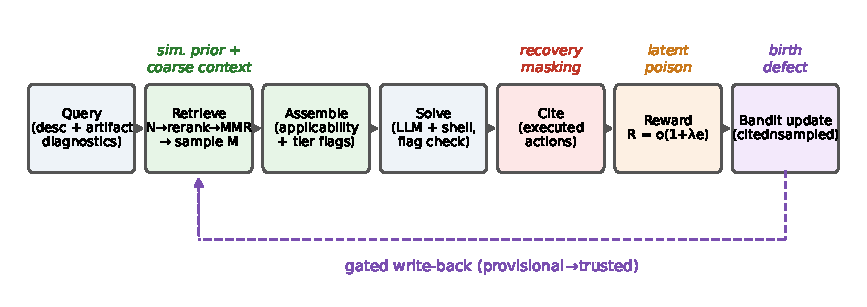
\includegraphics[width=0.96\textwidth]{fig_pipeline.pdf}
\caption{The solve-and-update loop. Each false-lesson lever (italics) attaches to
one stage: a coarse contextual bandit with a similarity prior controls
\emph{which} lessons are sampled; action-grounded credit (cited$\cap$sampled)
attacks \emph{recovery masking}; the step-count reward attacks \emph{latent
poison}; gated write-back attacks \emph{birth defects}. Every sampling decision is
logged with its propensity for off-policy evaluation.}
\label{fig:loop}
\end{figure*}

\section{Method}\label{sec:method}
The system retrieves a small set of lessons, solves with shell tools in a
container, then updates a contextual bandit over the graph and optionally writes
new lessons back. Figure~\ref{fig:loop} (and the released code) gives the full
pipeline; here we describe the four false-lesson levers.

\paragraph{Coarse contextual bandit (birth-of-signal).}
Per \texttt{(context $c$, lesson $v$)} the bandit stores a value $Q[c][v]$ and an
effective count $n[c][v]$. The context $c$ is a \emph{coarse} node---a CTF
category or a $k$-means cluster over challenge embeddings---\emph{not} a
per-challenge identifier. A per-challenge context yields fewer than one update per
cell within any realistic run budget and cannot learn; a sample-efficiency
calculation (expected updates per cell $=\,$runs$\cdot M/(|c|\cdot$credited$)$)
gates the granularity. The sampling score keeps similarity as a decaying prior:
\begin{equation}
\mathrm{score}(c,v)=\frac{n[c][v]\,Q[c][v]+\kappa\,\mathrm{prior}(v)}{n[c][v]+\kappa},
\end{equation}
where $\mathrm{prior}(v)$ is the query--lesson cosine on the reward scale and
$\kappa$ controls how many observations override similarity. A cold lesson is
sampled by its similarity, not an arbitrary uniform weight. We sample $M$ lessons
without replacement by sequential softmax at temperature $\tau$ and log the
per-draw propensity (below).

\paragraph{Step-count reward (latent poison).}
With outcome $o\in\{0,1\}$ and per-cell standardized steps $z$, efficiency is
$e=-z$ and the run reward is
\begin{equation}
R = o\,(1+\lambda e).
\end{equation}
A slow success earns $R<1$, a fast success $R>1$. A false lesson that wins via a
longer route therefore accrues a lower $Q$ than the correct method, and is
down-weighted---without any label beyond the flag and the step count. Steps, not
wall-clock, are used because wall-clock on a shared GPU is irreproducible.

\paragraph{Action-grounded credit (recovery masking).}
A sampled lesson $v$ is \emph{cited} iff its invocation signature (tool name,
technique keywords, or produced artifact) appears in the agent's executed shell
commands. Credit is assigned only to the cited subset $S=\text{sampled}\cap
\text{cited}$:
\begin{equation}
Q[c][v] \mathrel{+}= \alpha\,g(d_v)\,\big((R-b)-Q[c][v]\big),\quad v\in S,
\end{equation}
with $b$ the running mean reward in $c$ and $g(d_v)$ a distance scaling. A lesson
that merely sat in context during a success gains nothing---exactly denying the
credit that recovery masking would otherwise capture. We do \emph{not} use the
model's self-report of which lessons it ``used.''

\paragraph{Gated write-back (birth defect).}
New lessons distilled from a trajectory enter as \emph{provisional}: retrievable
but weight-capped and flagged low-confidence in context. A provisional lesson is
promoted to \emph{trusted} only after it is cited in $\ge k$ successful runs across
$\ge c$ distinct challenges. An $N{=}1$ lesson is therefore never trusted
prematurely. Failures are decomposed too (tagged), and every new node carries a
provenance edge and applicability conditions. Persistently-bad nodes are demoted
rather than deleted, preserving an audit trail.

\paragraph{Logging and off-policy evaluation.}
Every run logs the candidate pool with its score components, the realized
sampled set, the \emph{per-draw} sampling propensities, and the sequential set
log-probability. This makes the scarce GPU go further: an alternative policy
$\pi'$ (different $M,\tau,\kappa$) is scored on already-collected runs by
importance weighting, $w_i=P_{\pi'}/P_{\pi_{\log}}$, with inverse-propensity and
doubly-robust estimators \citep{OfflineEval,DoublyRobust}. We also implement a
leave-one-out causal probe \citep{MemoryR2}, in the process-reward-via-rollout
tradition of \citet{MathShepherd}: re-rolling a solve with
and without a suspect lesson, from a shared state, credits its \emph{marginal}
flag-reaching value---the oracle-free ground truth for false-lesson exposure.

% ===================================================================
% New method core: causal credit via the free randomized experiment.
% Integrated into main.tex once the campaign numbers land.
% ===================================================================

\section{From a Boundary to a Causal-Credit Construction}\label{sec:solution}
The levers of \S\ref{sec:method} run into a sharp boundary at \emph{recovery
masking} (\S\ref{sec:problem}). Action-grounded credit denies value to a false
lesson that is never executed, and the step reward down-weights one that wins by a
longer route; but a false lesson the agent \emph{executes} and then recovers from
receives the same verifiable-success credit as a genuinely useful one, because the
flag credits whichever tool was run. The information needed to tell them
apart---\emph{would the run have succeeded without this lesson?}---is simply not in
the scalar outcome of a single trajectory. \S\ref{sec:results} confirms this
empirically: the outcome bandit's learned value cannot separate executed poison from
true lessons. This section gives the construction that can.

Our key observation is that this counterfactual is, in principle, \emph{estimable for
free} in exactly this setting, for two reasons that coincide only in a verifiable-reward
agentic-memory system. How far that estimability actually \emph{reaches}---large helpful
effects yes, the per-item harm of a benign-false lesson no---is the subject of
\S\ref{sec:results2} and the identification analysis of \S\ref{sec:identifiability}. Here
we give the construction, which rests on two facts that coincide only in this setting:

\begin{enumerate}\itemsep2pt
\item \textbf{Stochastic retrieval is a randomized experiment.} Whether lesson $v$
  enters a run's context is the outcome of a stochastic softmax draw whose marginal
  inclusion propensity $\pi(v\mid c)$ is \emph{recoverable from the logs} (we log the
  per-candidate scores and temperature and Monte-Carlo-estimate $\pi$; \S\ref{sec:obs}).
  Lesson inclusion is thus a stochastically assigned treatment with an estimable
  propensity---the textbook ingredient for causal identification, here approximate
  rather than closed-form.
\item \textbf{The reward is verifiable and re-checkable.} Re-running a solve and
  checking the flag costs compute but needs \emph{no oracle}. So the counterfactual
  ``reward without $v$'' is directly measurable.
\end{enumerate}

\noindent We therefore replace the confounded outcome signal with a \emph{causal}
credit signal---the lesson's marginal effect on reward---in three forms that trade
cost against precision.

\subsection{Active causal credit (leave-one-out re-rollout)}\label{sec:active}
For each lesson $v$ cited (executed) on a run, re-solve the same challenge from the
same state with $v$ \emph{removed} from context, holding all other sampled lessons
fixed, averaged over $s$ independent re-rolls (the solver is stochastic; one re-roll
is a coin flip). Credit $v$ with the marginal reward
\begin{equation}
\Delta R(v) \;=\; R_{\text{with}} \;-\; \tfrac{1}{s}\textstyle\sum_{j} R_{\text{without}}^{(j)},
\end{equation}
where $R=o\,(1{+}\lambda e)$ includes the step-count efficiency term, so a lesson the
agent recovers from but is \emph{slowed} by earns a negative marginal even when the
outcome is unchanged (latent poison). This is precise but costs $s$ extra solves per
cited lesson; we gate it to cited lessons and report the re-roll budget.

\subsection{Observational causal credit (inverse-propensity weighting)}\label{sec:obs}
The re-rolls are unnecessary when the data already contains the experiment. Over many
runs, $v$ is sometimes in context (treated) and sometimes not (control), with logged
inclusion propensity $\pi_i(v)$ on run $i$. The marginal value of $v$ is the
\emph{self-normalized inverse-propensity-weighted} (SNIPW) contrast
\begin{equation}\label{eq:snipw}
\widehat{\mathrm{ATE}}(v\mid c)=
\frac{\sum_{i:\,v\in M_i} R_i/\pi_i(v)}{\sum_{i:\,v\in M_i} 1/\pi_i(v)}
-
\frac{\sum_{i:\,v\notin M_i} R_i/(1{-}\pi_i(v))}{\sum_{i:\,v\notin M_i} 1/(1{-}\pi_i(v))},
\end{equation}
estimated within each context $c$ and shrunk toward the node's global estimate for
sparse cells (partial pooling). $\pi_i(v)$---the marginal probability $v$ is among
the $M$ sampled without replacement---is computed by Monte-Carlo from the logged
per-candidate scores and temperature. This uses \textbf{no additional inference}: it
reads the same logs the outcome bandit was fooled by. It recovers \emph{large} marginal
effects---the helpful lessons outcome credit conflates with poison---reliably; whether
it recovers the \emph{small} per-item harm of a benign-false lesson is exactly the
identification question \S\ref{sec:identifiability} answers in the negative.

\subsection{The online observational bandit}\label{sec:onl}
Equation~\ref{eq:snipw} yields a deployable system. The bandit samples lessons via the
similarity-blended score as before, logging propensities; after each epoch it
\emph{recomputes} its value table $Q[c][v]\leftarrow\widehat{\mathrm{ATE}}(v\mid c)$
from its own accumulated logs and performs no per-run updates. The randomization that
drives identification is the very exploration the bandit already does, so the credit
signal is causal by construction at zero marginal cost. Active re-rolls
(\S\ref{sec:active}) then serve as an expensive but assumption-light validation of
the cheap estimator: because they hold the other sampled lessons fixed, they are
robust to the interference that the observational estimator must marginalize over,
so agreement between them bounds the interference error.

\paragraph{Why this is the right tool for verifiable-reward memory.} In an
open-ended domain neither ingredient holds: lesson inclusion is rarely randomized
with a known propensity, and the reward cannot be re-checked without an oracle. The
verifiable-reward agentic-memory setting is special precisely because it supplies
both---so the false-lesson problem that is intractable in general becomes, here, an
estimation problem with a free experiment attached. ``Estimable,'' though, is not
``solved'': \S\ref{sec:identifiability} shows the per-item harm of a benign-false lesson
is non-identifiable even with the experiment in hand, so the construction's value is the
large helpful effects it does recover and the sharp boundary it lets us draw.


\section{Experimental Setup}\label{sec:setup}
\paragraph{Why a controlled corpus.} Live public CTF challenges confound two
things we must separate: pretraining contamination (the model has seen the flag)
and the absence of ground-truth causal labels (we cannot know \emph{which} lesson
caused a solve). We therefore build a corpus of small, automatically-verifiable
tasks. Each task embeds a \emph{freshly random} flag \texttt{picoCTF\{$\cdots$\}},
so the model cannot have memorized it (zero contamination), and each family has a
\emph{known} correct method plus a planted \emph{poison} lesson naming a
plausible-but-wrong method. Descriptions are method-neutral, so a retrieved
lesson---not the prompt---carries the method.

\paragraph{Calibrating the corpus to the solver (the key design step).} A controlled
corpus only measures false-lesson dynamics if it sits in the band where a lesson
\emph{matters}: too easy and the model solves regardless (a poison cannot hurt, a
true lesson cannot help); too hard and it fails even with the true lesson. A
first-pass corpus (\S\ref{sec:results}) was bimodal for our 4B solver---trivial
single decodes at ceiling, exact-crypto families at floor---so we recalibrate. Each
family is now a two-layer decode in which an \emph{outer} transport encoding
(Base64 or hex, so \texttt{file} on the artifact reveals only ``ASCII text'') wraps
an \emph{inner} transform (gzip, raw zlib, single-byte XOR, or reverse) that is
invisible in the raw bytes. The model can execute each step but cannot guess the
inner transform from the artifact, so the retrieved \emph{recipe} carries the
method: the true lesson names the right inner transform; the poison names a
plausible wrong one. The round budget is kept tight (four) so the model cannot
simply explore every decoding. This yields the regime the study needs---the true
lesson lifts solve sharply over no memory, and a poison co-retrieved with it is the
clean instance of recovery masking. We use the families the 4B executes reliably
once instructed (\texttt{b64\_gzip}, \texttt{b64\_rev}) plus harder zlib/XOR variants
where it succeeds only sometimes, spanning an easy--hard difficulty range.

\paragraph{Model substitution (disclosed).} The intended lab solver was
Qwen3.5-27B-FP8 on dual A5000s (ultimately not run; the lab-scale ladder below uses
Qwen2.5). The pilot runs on a single 8\,GB laptop GPU, on which that model is
infeasible; we substitute \textbf{Qwen3-4B-Instruct-2507} in 4-bit---a smaller model
of the \emph{same family} as the intended Qwen3.5 solver, one release apart---served behind the same
OpenAI-compatible API the solver already uses, with a small bi-encoder (all-MiniLM)
as the retrieval embedder. The rerank stage in every reported run is a deterministic
lexical-overlap-plus-cosine reranker, not a trained cross-encoder (which the code
supports but we did not need): in the controlled corpus each family's true and poison
lessons are on-target and dominate query similarity by construction, so which lessons
reach the sampled $M$-set---and thus every logged propensity the causal estimators
use---does not depend on the reranker's sophistication. The same-family choice is deliberate but limited: the
spurious-reward effect is documented for the Qwen family specifically
\citep{SpuriousRewards}, and self-preference bias affects LLM-as-judge setups
generally \citep{JudgingTheJudges}; a Qwen-3-generation pilot shares the solver
family but \emph{not} the capability of the 27B lab model, and capability-dependent
false-lesson dynamics may not transfer (\S\ref{sec:disc}). This is a capability
substitution, not a method change; we report mechanism
and lift. A calibration run placed the solver's no-memory solve rate near the middle
of the range (\BzeroSolve{}), giving headroom for lessons to help \emph{and} for
poison to harm---the regime the study needs.

\paragraph{The lab-scale ladder (where the headline lives).} The 4B pilot
\emph{illustrates} the boundary and the credit-signal failure mode; the load-bearing
non-identifiability evidence---the active leave-one-out gold standard (\S\ref{sec:results2}),
the positive control, the capability ladder, and the base-rate floor of
\S\ref{sec:identifiability}---comes from a separate set of \emph{lab-scale} campaigns that
run the same instrument and pipeline at $M{=}3$. The ladder is the \textbf{Qwen2.5-Instruct}
family---3B, 7B, 14B-AWQ, 32B-AWQ---plus a non-Qwen rung
(\textbf{Llama-3.1-8B-Instruct}); the rungs log $2.2$k--$15.6$k runs over $11$--$43$
challenge families each (${\sim}15.6$k/$15.5$k at the powered 14B/32B rungs, over $41$/$43$
families), and a malignant positive-control campaign (14B, $4264$ runs, later expanded by a
further $5096$) adds the actively-destructive lesson types. We are explicit that this ladder is a \emph{different
model generation} from the Qwen3-4B pilot (and from the intended-but-unrun Qwen3.5-27B lab
solver): the cross-rung consistency we report is therefore \emph{within} the Qwen2.5 family
plus one Llama rung, not across the pilot's generation, and ``across architecture'' means
the single Llama rung (other non-Qwen probes were harness-floored at $n\le3$;
\S\ref{sec:disc}).

\paragraph{Baselines and ablations.} \textbf{B0}: no graph (the lift denominator).
\textbf{B2}: static similarity retrieval with reranking and diversity, no bandit.
\textbf{B4}: the full method (bandit, cited-only credit, step reward). We ablate
the two oracle-free levers: \emph{all-$M$ credit} (credit every in-context lesson,
not just cited ones) isolates recovery masking, and \emph{outcome-only reward}
($\lambda{=}0$) isolates latent poison. \textbf{B5/B6}: gated vs.\ ungated
write-back. Each learning system streams the corpus for two epochs; B4 is then
frozen and evaluated paired against B0/B2 on common random seeds.

\paragraph{Metrics and statistics.} Solve rate and paired lift over B0 with
bootstrap confidence intervals and exact McNemar tests
\citep{PairedBootstrap,ErrorBarsToEvals}; mean learned $Q$ by ground-truth lesson
label; poison citation rate and recovery-masking rate; and the leave-one-out
marginal value (false-lesson exposure). Difficulty is ground-truth (family point
value); the bandit budget calculation is reported.

\section{Results: The Boundary}\label{sec:results}
% Pilot boundary on the v1 micro-CTF corpus; macros from paper/numbers.tex.
\noindent We first report a pilot on an initial micro-CTF corpus. It establishes the
boundary the rest of the paper addresses and, in doing so, exposes the
benchmark-calibration lesson that motivates the recalibrated corpus
(\S\ref{sec:setup}) used for the causal-credit study in \S\ref{sec:results2}.
% Results body — finalized against results/pilot/analysis.json; numbers are macros
% from numbers.tex (each traces to the JSONL logs). We deliberately report the
% boundary (what the verifiable signal cannot do) as prominently as the positives.
We report findings in four parts. All paired comparisons use common random seeds
and bootstrap confidence intervals; we report the headline comparison at the
\emph{challenge} level (independent units) because our \Npairs{} rows are
\NchalPairs{} challenges $\times$ two seeds, and the seeds are highly correlated
(identical B0 outcome on \SeedAgree{}/\NchalPairs{} challenges).

\paragraph{(1) Retrieval helps, but the lift is concentrated.}
Static retrieval (B2) reaches \BtwoSolve{} vs.\ \BzeroSolve{} with no memory---a
paired lift of \BtwoLift{} that remains significant at the challenge level
($p\eqd\BtwoLiftChalP{}$, \NchalPairs{} challenges, a challenge counted solved if
solved under either seed: exact McNemar over the six discordant challenges, all
favoring B2; Table~\ref{tab:main},
Fig.~\ref{fig:solve}). The lift is \emph{not} uniform: \NCeiling{} of ten families
are already solved with or without memory and \NFloor{} are unsolved in both
conditions, so the entire effect comes from \NLift{} families (ROT13, reverse,
and the two-layer Base64$\circ$ROT13). The lessons carry value precisely where the
model is neither saturated nor blocked. This concentration is itself the reason
false-lesson propagation is worth studying here: a memory that helps on a few
families can still accrue incorrect lessons that the aggregate solve rate hides.
(The methodological note stands regardless: the prior between-subjects evaluation
reported a comparable effect that was not significant; the paired design resolves
it.)

\begin{table}[t]\centering\small
\setlength{\tabcolsep}{3.5pt}
% main results (Phase A + B)
\begin{tabular}{lccc}\toprule
System & Solve rate & Lift vs B0 & 95\% CI \\\midrule
B0 (no graph) & 0.54 & --- & --- \\
B2 (static retrieval) & 0.66 & +0.12 & [+0.05,+0.21] \\
B4 (bandit, full) & 0.61 & +0.07 & [+0.00,+0.15] \\
\bottomrule\end{tabular}

% ablation table (Phase B)
\begin{tabular}{lccc}\toprule
Config & Q(true) & Q(poison) & Q(distractor) \\\midrule
cited-only + step (full) & +0.34 & +0.40 & +0.00 \\
all-$M$ credit & +0.29 & +0.29 & +0.36 \\
outcome-only reward & +0.37 & +0.40 & +0.00 \\
\bottomrule\end{tabular}
\caption{Top: solve rate and challenge-level paired lift over no memory
(B4 is the frozen bandit and does \emph{not} beat B2). Bottom: final learned value
$Q$ of true, poison, and unused (distractor) lessons under each configuration.
The bandit values executed poison indistinguishably from true lessons at this $n$.}
\label{tab:main}
\end{table}

\paragraph{(2) Action-grounded credit zeroes \emph{unused} false lessons.}
Cited-only credit assigns no update to a lesson that emitted no command, so unused
(distractor) lessons stay at the prior, $Q\eqd\QdistractCited{}$, whereas all-$M$
credit rewards them on every success, $Q\eqd\QdistractAllM{}$ (Fig.~\ref{fig:qcfg}).
This zeroing follows directly from the update rule; the \emph{empirical} content is
the magnitude of spurious credit it withholds---a \RecovMask{} recovery-masking
rate, i.e.\ that fraction of in-context lessons present during a success were never
executed and would have been credited by all-$M$. So the lever genuinely matters
for the \emph{passive} mode, but its effect is mechanical, not learned.

\begin{figure}[t]\centering
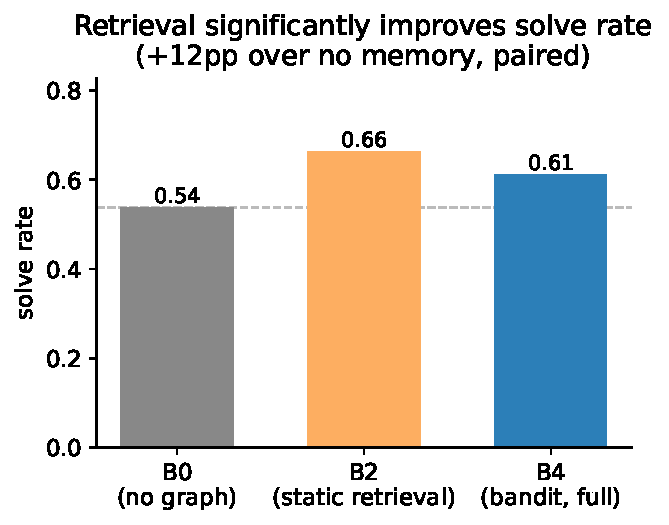
\includegraphics[width=0.86\linewidth]{fig_solve_rates.pdf}
\caption{No memory (B0) vs.\ static retrieval (B2) vs.\ the frozen bandit (B4).
Retrieval lifts solve rate; the bandit (B4) does \emph{not} improve on static
retrieval at this scale---its interest is in \emph{what it learns about lessons}.}
\label{fig:solve}
\end{figure}

\begin{figure}[t]\centering
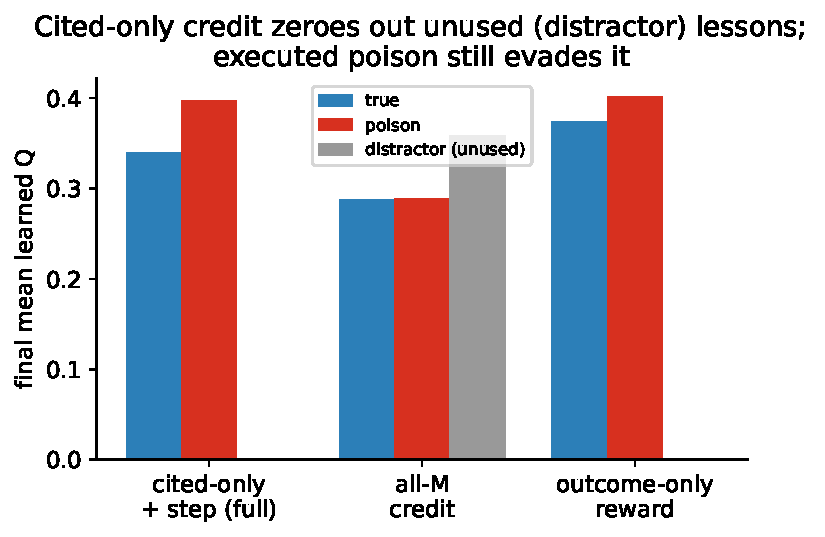
\includegraphics[width=0.96\linewidth]{fig_q_by_config.pdf}
\caption{Final learned value by ground-truth lesson type. Cited-only credit holds
\emph{unused} (distractor) lessons at zero; all-$M$ credit rewards them. But
\emph{executed} poison keeps a value indistinguishable from true lessons under every
configuration ($n{=}4$/label)---outcome credit cannot tell them apart.}
\label{fig:qcfg}
\end{figure}

\paragraph{(3) Executed poison evades the verifiable signal.}
When the false lesson is itself executed, cited-only credit cannot help. Poison
lessons name a wrong tool the agent runs (cited on \PoisonCite{} of the runs they
are sampled in); on a \emph{recovered} success they receive the same positive
credit as a useful lesson. The bandit therefore values poison
indistinguishably from true lessons ($Q_{\text{poison}}\eqd\Qpoison{}$, in this pilot
corpus numerically above $Q_{\text{true}}\eqd\Qtrue{}$; Fig.~\ref{fig:qtraj}), and the frozen bandit
does not beat static retrieval (\BfourSolve{}). The step-count lever does not
change this ($Q_{\text{poison}}\eqd\QpoisonOutcome{}$ under outcome-only reward as
well)---but for a reason that is itself a limitation: this corpus's poison misleads
via the \emph{wrong tool}, not a longer route, so the latent-poison mode the
step-count reward targets is never instantiated here, and that lever is
\emph{specified but not empirically tested} (\S\ref{sec:disc}). The clean statement
is: a verifiable success credits whichever tool was run, true or false; the
verifiable signal alone, even with action-grounded credit, does not attribute cause.

\begin{figure}[t]\centering
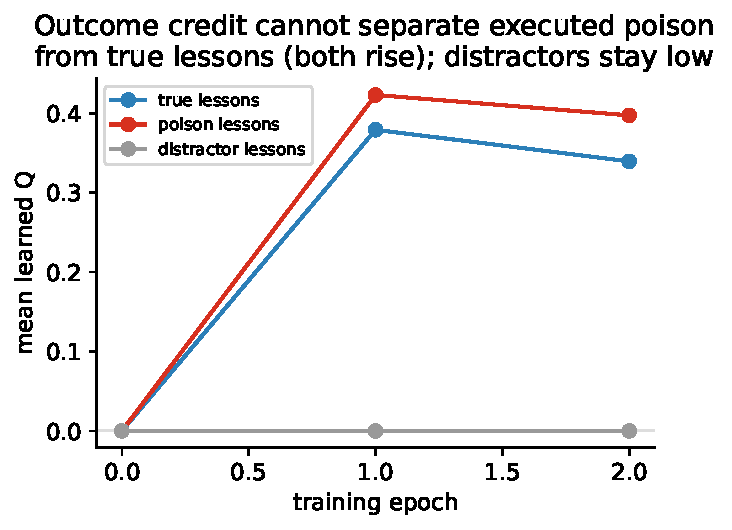
\includegraphics[width=0.86\linewidth]{fig_q_trajectory.pdf}
\caption{Learned value over training (full method). Executed poison tracks true
lessons---outcome credit cannot separate them---while unused distractors stay at
zero.}
\label{fig:qtraj}
\end{figure}

\paragraph{(4) An oracle-free causal probe measures marginal necessity.}
The leave-one-out re-rollout probe re-solves a challenge with and without a single
lesson, from a shared state, using only the flag. It measures single-lesson
\emph{necessity}; whether it can \emph{rank} the small per-item harm of a benign-false
lesson is a separate question that the lab-scale battery answers in the negative
(\S\ref{sec:results2}). On the ten probed
challenges---one true and one poison lesson each, twenty challenge--lesson pairs
(drawn from \emph{five} of the ten families: Base64, hex,
ROT13, reverse, gzip---the python-scripted families XOR and Caesar, and the
largest lift driver Base64$\circ$ROT13, are \emph{not} probed)---poison lessons
have marginal contribution
$\Delta\text{solve}\eqd\LooPoison{}$, while true lessons have $\eqd\LooTrue{}$.
That mean is bimodal: true lessons are causally \emph{necessary}
($\Delta\text{solve}\eqd{+}1.0$) only on the families the model cannot solve
unaided (ROT13, reverse) and $0$ where it already succeeds---so the probe measures
genuine necessity, not correlation with success. Two caveats are essential and we
state them plainly. First, the probe and the bandit $Q$ are different estimands
(single-lesson necessity vs.\ average reward over an $M{=}8$ context), so part of
the apparent ``probe succeeds where $Q$ fails'' gap is the change of estimand;
second, because our poison is a non-reaching wrong tool, its non-causality is
\emph{partly true by construction}---the stronger test has two halves: poison that
reaches the flag by a longer route, which we construct in Appendix~\ref{app:latent} and
probe against the \emph{step} channel only (the LOO probe was not run against it), and
LOO at matched $M{=}8$ conditioning, which remains future work.
The two remaining levers behave \emph{as specified}: gated write-back leaves
\GatedProvPct{} of new lessons (\GatedProv{}/\GatedTotal{}) provisional and trusts only
\GatedTrust{}/\GatedTotal{}, against \UngatedTrust{}/\UngatedTotal{}
(\UngatedTrustPct{}) trusted under ungating---though we report the provisional/trusted
split, not whether the trusted nodes were causally correct. Finally, off-policy evaluation recovers the logging policy's measured
value (doubly-robust \OpeDR{} vs.\ measured \OpeMeasured{}); this sanity check is
exact because the importance weights are unity when $\pi'\!=\!\pi_{\log}$, so it
\emph{validates the estimator} rather than identifying a better policy---the top
counterfactual temperature ($\tau\eqd\OpeBestTau{}$) lies within the logging
policy's CI (Fig.~\ref{fig:ope}). Validating under genuine distribution shift
requires a second on-GPU batch and is future work.

\begin{figure}[t]\centering
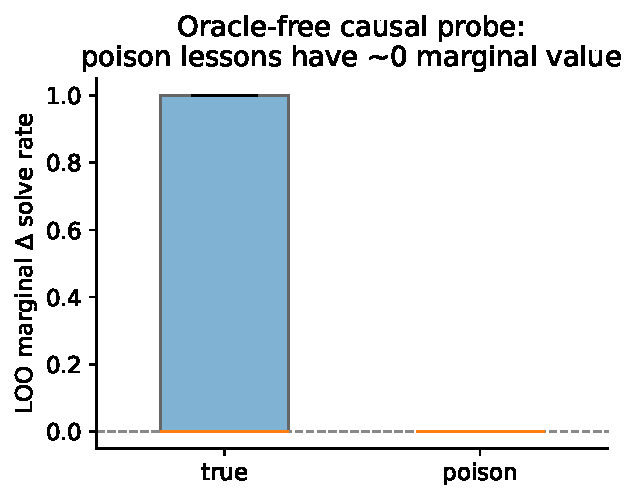
\includegraphics[width=0.74\linewidth]{fig_loo.pdf}
\caption{Leave-one-out marginal contribution, by ground-truth lesson type, on the
five LOO-probed families. Poison shows $\Delta\!\approx\!0$ here---partly true by
construction (a non-reaching wrong tool), and its small \emph{per-item} effect is not
rankable at scale (\S\ref{sec:results2})---where the bandit's outcome-credit had valued
it like a true lesson; true lessons are causal only where the model cannot already solve
unaided.}
\label{fig:loo}
\end{figure}

\begin{figure}[t]\centering
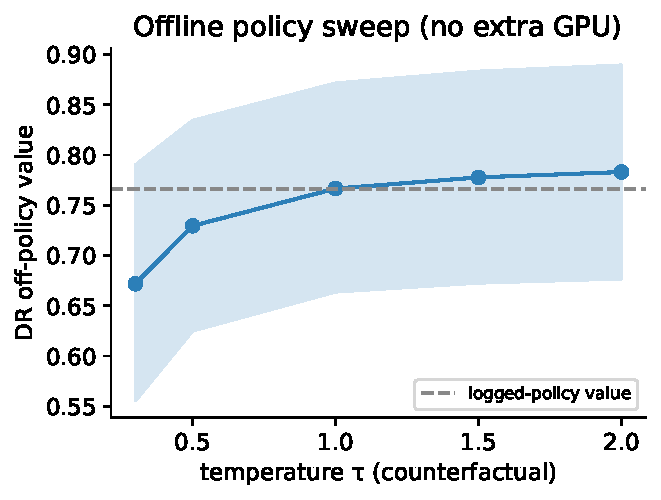
\includegraphics[width=0.82\linewidth]{fig_ope_sweep.pdf}
\caption{Off-policy value of counterfactual sampling temperatures from logged
propensities. The doubly-robust estimate recovers the logging policy's measured
value (dashed); the top candidate is within its CI, so the sweep validates the
estimator without identifying a significantly better policy at this $n$.}
\label{fig:ope}
\end{figure}

\paragraph{Summary.} The verifiable flag, with action-grounded credit, cheaply
removes value from \emph{unused} false lessons and (with gating) withholds trust
from \emph{premature} ones, but \emph{cannot} down-weight executed false lessons
the agent recovers from---the engineered bandit therefore does not improve on
static retrieval here. A causal re-rollout measures single-lesson necessity on the
subset we probe---and \S\ref{sec:results2} pushes this to its limit, showing that even
this gold standard cannot rank the per-item harm of a benign-false lesson. This maps
which false-lesson modes the verifiable signal alone can contain, and where causal credit
reaches and where it does not.

\section{Results: What Verifiable Credit Can and Cannot Identify}\label{sec:results2}
% v2 causal-credit study on the recalibrated corpus; macros from numbers_solution.tex.
% ===================================================================
% Solution results, rewritten 2026-06-26 to the honest non-identifiability
% framing (docs/CLAIMS_v2.md). The retracted thesis ("the observational
% estimator recovers a reliable poison-negative the write-back gate needs")
% is GONE. Numbers: 4B-campaign macros from numbers_solution.tex
% (experiments/analyze_campaign.py over results/campaign_v2/); the
% gold-standard LOO + positive control + ladder numbers are lab-scale and
% inlined with per-number provenance comments (same convention as the
% theorem section). Every inline number traces to a committed artifact.
% ===================================================================

We instantiate the credit signals on the recalibrated corpus
(\S\ref{sec:setup}): \textbf{B0} (no memory), \textbf{B2} (static similarity
retrieval), \textbf{outcome} (the bandit with outcome credit), and
\textbf{observational} (the online observational causal bandit, \S\ref{sec:onl}); an
active leave-one-out re-rollout (\S\ref{sec:active}) serves as the assumption-light
\emph{gold standard} against which we judge the cheap signals. Each learning condition
streams the \CampNtrain{} training challenges for \CampEpochs{} epochs, is then frozen,
and is evaluated paired against the others on the \CampNheldout{} held-out instances
over \CampEvalSeeds{} seeds. The held-out set and seeds are identical across
conditions, so every contrast below is within-item paired (bootstrap CI + exact
McNemar). Rows are instance$\times$seed and seeds are positively correlated, so these
campaign $p$-values are anti-conservative; no campaign-level contrast is claimed
significant. The gold-standard re-rollout, the positive control, and the capability
ladder are established at \emph{lab scale} on the same instrument (the high-$n$
campaigns, e.g.\ \texttt{campaign\_14b\_M3\_powered}, $n{\approx}15.6$k); we say so at
each use. One provenance caveat: the 4B campaign itself ran on an earlier benchmark
revision (poison-contract / oracle-labeling / grid-duplication bugs fixed later in commit
\texttt{63db02d}) and was \emph{not} re-run, so the 4B magnitudes below are illustrative of
the failure mode---the load-bearing non-identifiability evidence is the lab-scale ladder,
not the 4B numbers.

\paragraph{The boundary, reproduced on real logs.} Outcome credit cannot tell an
executed-but-recovered-from poison lesson from a useful one. Over the full training
stream it learns a mean $Q$ of \OutQTrue{} for true lessons and \OutQPoison{} for
poison: it ranks true lessons only slightly higher (gap
\OutQGap{}, $n{=}4$/label---too few for a formal test) and assigns poison
a clearly \emph{positive} value, because a verifiable success credits whichever lesson
was in context and the poison's claimed action (\texttt{base64}) is part of the correct
recipe it cannot be denied credit for. An outcome-credit memory therefore holds no
internal signal that executed poison is anything but a useful lesson---the failure mode
this paper is about.

\paragraph{The free experiment identifies the \emph{helpful} lessons.} The same logs
contain a free randomized experiment: each lesson's inclusion is a stochastic draw with
a logged propensity (\S\ref{sec:obs}). Re-scoring \emph{those same} outcome-condition
runs with the observational SNIPW estimator (\S\ref{sec:obs})---no extra inference---recovers
the value of the helpful lessons outcome credit conflates with poison: the mean IPW ATE
on reward is \ObsAteTrue{} for true lessons, a large positive effect, with distractors
at \ObsAteDistract{}. This large helpful effect is where the agent's own exploration
\emph{does} suffice to credit a lesson causally for free, and it is corroborated by the
gold standard: at lab scale the active re-rollout ranks the helpful lessons in strong
agreement with the cheap estimate (within-helpful rank correlation $+0.64$, CI
$[+0.34,+0.85]$; the gold
standard orders $30/30$ helpful nodes)%
\footnote{Lab-scale, \texttt{campaign\_14b\_M3\_powered}; emitted by
\texttt{experiments/within\_poison\_validation.py} into \texttt{active\_loo\_within\_label.json}.}
and the helpful on-target solve ATE (the \emph{on-target} contrast restricts the run
set to challenges of the lesson's own family---family is pre-treatment---as opposed to the
\emph{marginal-inclusion} effect of merely placing it in the retrieved $M$-set) is large at every rung and markedly larger at the
high-capability Qwen rungs
($+0.247/{+}0.195/{+}0.526/{+}0.570/{+}0.227$ at 3B/7B/14B/32B/Llama-8B, all $p<.001$;
\S\ref{sec:identifiability}). This is the \emph{positive} half of the boundary.

\paragraph{\ldots but not the per-item harm of a poison lesson.} The negative half is
the paper's central result. The same observational estimator reads poison only
\emph{mildly} negative---\ObsAtePoison{} on this 4B campaign, and at higher capability
with far more data a small $-0.057$ ($p{<}.001$, CI $[-0.087,-0.022]$) at 14B and $-0.064$
($p{=}.005$, CI $[-0.109,-0.018]$) at 32B---the pre-registered per-rung primary contrast
at each rung; the 14B/32B cells survive Benjamini--Hochberg at $q{=}.05$ across the five
rungs, the other rungs are null (all other grid cells are exploratory). These are the \emph{on-target} contrasts; the marginal-inclusion ATE is null at
every $M$ (\S\ref{sec:disc}).%
\footnote{Lab-scale on-target SNIPW, \texttt{campaign\_14b\_M3\_powered} and \texttt{campaign\_32b\_M3\_tp2}
(\S\ref{sec:identifiability}).}
That sign is \emph{not} the per-item causal harm (Fig.~\ref{fig:sep}). Against the assumption-light active
leave-one-out gold standard---which re-solves each challenge with and without a single
lesson, holding the others fixed---the cheap estimate cannot \emph{rank} the per-item
poison effect: within poison, the rank correlation between the cheap estimate and the
gold standard is $\approx 0$ ($+0.072$ tie-corrected Spearman, $+0.028$ rank-Pearson;
wide bootstrap CI $[-0.35,+0.49]$, emitter-backed, seed 0), and among the lessons the
gold standard can order
at all, the two agree on the \emph{sign} of only $8$ of $18$ ($p{=}0.76$, one-sided
exact binomial against chance $0.5$---at chance,
not anti-correlated).%
\footnote{\texttt{experiments/within\_poison\_validation.py}; the often-quoted ``$8/28$''
counts $10$ gold-standard ties-at-zero (a $1/12$-quantized estimate) as disagreements.}
The reason is not merely that the cheap estimator is noisy: the feasible-$n$ gold
standard \emph{itself} cannot resolve the small poison effects. Its mean poison marginal
is $+0.045$ ($n{=}28$ lessons), $95\%$ CI $[-0.006,+0.098]$---a fail-to-reject,
\emph{ill-posed}, never a
measured ``zero''---and its per-node standard error (a worst-case $p{=}0.5$ binomial
bound at the deployed re-roll budget, $\approx0.20$) exceeds the between-node spread of
the effects it must rank ($0.14$). \textbf{Neither} signal
identifies the per-item harm---and if anything this understates the difficulty: the
active-LOO contexts themselves rendered the poison lesson \emph{first}, biasing its
per-item effect toward looking \emph{more} harmful, so the gold standard's inability to
rank it is conservative. The mildly-negative observational sign is a real
\emph{label-level} regularity but a confounded one---\S\ref{sec:identifiability} derives
its source under the measured base-rate floor---and it is neither the per-item causal
estimand nor, as we show below, a signal a write-back gate can be built on.

\paragraph{A positive control: what verifiable credit \emph{can} catch.} The
non-identifiability is specific to a \emph{benign}-false lesson the agent recovers from,
not a blanket failure of the estimator. We additionally plant two \emph{actively
destructive} lesson types that push the outcome \emph{below} the base-rate
floor---one that destroys working state (\textsf{destroy}) and one that burns the round
budget (\textsf{exhaust})---a \textsf{wrongflag} lesson that confidently submits a wrong
answer, and a deterministic \textsf{verifier} that re-runs the cited recipe in
isolation. The SNIPW estimator \emph{detects} the floor-violating harms
(\textsf{destroy} ATE $\MalPoolDestroyAte{}$, two-sided $p{=}\MalPoolDestroyPtwo{}$,
CI $\MalPoolDestroyCI{}$, $\MalPoolDestroyNfam{}$ families; \textsf{exhaust}
$\MalPoolExhaustAte{}$, $p{=}\MalPoolExhaustPtwo{}$, CI $\MalPoolExhaustCI{}$,
$\MalPoolExhaustNfam{}$ families; both CIs excluding $0$, though the binary
\textsf{destroy} clears $p<.05$ only once campaigns are pooled---see note) but is \emph{untested} on \textsf{wrongflag}. The
agent executed that recipe on only $11$ of $453$ sampled runs (follow rate $0.024$,
against $0.978$ and $0.805$ for \textsf{destroy} and \textsf{exhaust}), so its
on-target SNIPW ($+0.004$, $p{=}.69$, $64$ families---the same pooled estimator and file
as \textsf{destroy}/\textsf{exhaust} above,
\texttt{malignant\_pooled\_combined.json}) carries almost no treated exposure: this
is a null from non-exposure, not a demonstrated blind spot. Under \emph{forced} exposure
the constructed leave-one-out does detect the arm ($-0.43$, CI $[-0.54,-0.32]$, $n{=}41$
families; direction and sign only---see note).\footnote{The \textsf{wrongflag} arm was
already toothless at the pre-registered probe---cited on $0$ of $42$ sampled runs
(\texttt{campaign\_14b\_malig\_probe/merged/malignant\_probe\_check.json})---which the
pre-registration required be redesigned before scaling. It was scaled unmodified; we log
this as a deviation and treat the arm as untested rather than as evidence of a blind
spot.} The execution-verifier flags invalid recipes on $100\%$ and valid ones on $0\%$ of
families \emph{by construction} (a deployable contrast on \emph{recipe validity}, not a
measured generalization; \S\ref{sec:identifiability}, Prop.~\ref{thm:recovery}). The
malignant campaign over-samples its planted lessons ${\sim}2.5\times$, which depresses the
base rate and makes the \emph{same-campaign} benign poison read spuriously positive
(run-level $+0.033$, one-sided $p{=}.0475$, two-sided $.095$)---so the benign-poison null is the
\emph{main}-campaign result, not this one---but \textsf{destroy}/\textsf{exhaust} are
floor-\emph{violating} and detected regardless.%
\footnote{Lab-scale malignant campaign, family-clustered SNIPW \emph{pooled} over
\texttt{campaign\_14b\_malig} + \texttt{campaign\_14b\_malig\_expand} ($74$/$71$ family
clusters in the \textsf{destroy}/\textsf{exhaust} contrasts);
the single-campaign binary \textsf{destroy} was borderline ($p{=}.057$) and the campaign
was expanded to power it, so the robust single-campaign evidence is the descriptive
within-family \textsf{destroy} ATE $-0.045$, CI $[-0.055,-0.032]$ (excludes $0$ without
pooling). The constructed direct-harm magnitudes are forced-exposure and
order-confounded, so they are direction/sign evidence, not clean effect sizes.}
This is the boundary in one experiment: outcome-based credit identifies large helpful
effects and actively-destructive harm, but \emph{not} the per-item harm of a
benign-false lesson, and it is \emph{untested} against a confidently-wrong answer.

\begin{figure}[t]
\centering
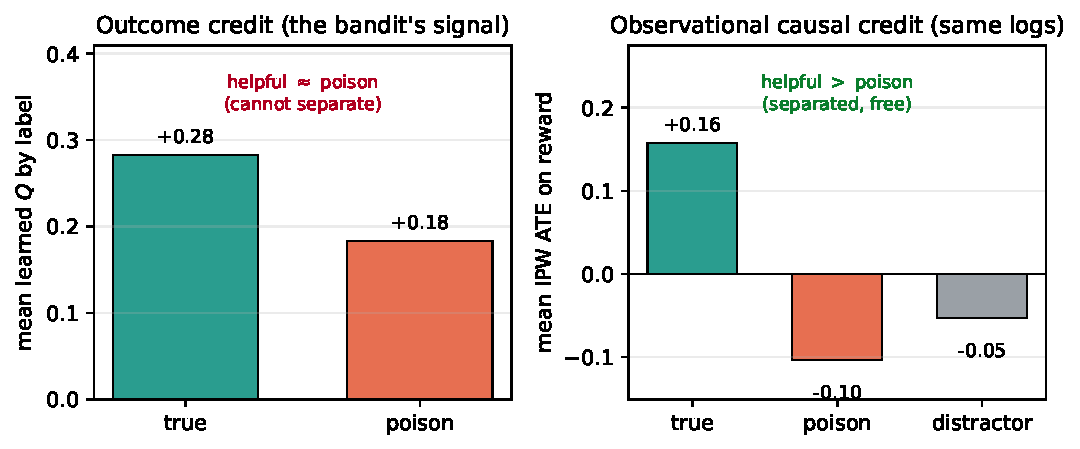
\includegraphics[width=0.92\linewidth]{fig_separation.pdf}
\caption{Same logs, two credit signals (4B recalibrated campaign, run on the earlier
pre-fix benchmark revision; magnitudes illustrative).
\emph{Left:} outcome-bandit $Q$ by ground-truth label---executed poison earns a positive
value, numerically beside true lessons. \emph{Right:} observational IPW ATE on the same
runs---poison mildly negative, true strongly positive. The mild negative is a confounded
label-level sign, \emph{not} a per-item poison detector (\S\ref{sec:identifiability}).}
\label{fig:sep}
\end{figure}

\paragraph{Held-out solve rate (parity, by design).} Table~\ref{tab:solve} reports
solve rates; the headline is \emph{not} here, and the next paragraph explains why it
should not be. Retrieval is directionally ahead of no memory (B2 \CampBtwo{} vs.\ B0
\CampBzero{}, paired \BtwoVsBzero{}, $p\eqd\BtwoVsBzeroP{}$---underpowered here; the
pilot's paired lift, \S\ref{sec:results}, is the significant version of this contrast),
consistent with the
recalibrated corpus putting the solver in a band where lessons matter. But the credit signals are not separated at this $n$: the
online observational causal bandit reaches \CampObs{} against the outcome bandit's
\CampOutcome{} (paired \ObsVsOutcome{}, McNemar $p\eqd\ObsVsOutcomeP{}$) and static
retrieval's \CampBtwo{} (paired \ObsVsBtwo{}). Whatever the credit signal, the bandit
retrieves the true lesson and the solver follows it, so solve rate does not separate
the signals---and, as we have shown, neither does any of them recover the per-item
poison effect.

\begin{table}[t]
\centering\small
\setlength{\tabcolsep}{5pt}
\begin{tabular}{lc}
\toprule
condition & held-out solve \\
\midrule
B0 (no memory)       & \CampBzero{} \\
B2 (static)          & \CampBtwo{} \\
outcome credit       & \CampOutcome{} \\
observational causal & \CampObs{} \\
\midrule
paired contrast & $\Delta$ (McNemar $p$) \\
\midrule
B2 $-$ B0                  & \BtwoVsBzero{} ($p\eqd\BtwoVsBzeroP{}$) \\
observational $-$ outcome  & \ObsVsOutcome{} ($p\eqd\ObsVsOutcomeP{}$) \\
observational $-$ B2       & \ObsVsBtwo{} ($p\eqd\ObsVsBtwoP{}$) \\
\bottomrule
\end{tabular}
\caption{Top: held-out solve rate by credit signal (4B campaign, run on the pre-fix
benchmark revision and not re-run---illustrative; see the provenance caveat opening
\S\ref{sec:results2}). Bottom: within-item paired
contrasts (McNemar). Retrieval lifts solve over no memory, but the credit signals
are not separated on solve rate at this $n$ (an underpowered fail-to-reject, not a measured
equality; both paired intervals are bounded above by $0.0$) (and, as the text shows, in any trustworthy
per-item poison value).}
\label{tab:solve}
\end{table}

\paragraph{Where the harm does and does not surface.} The credit signals are at parity
on \emph{immediate} held-out solve rate, expected on the \emph{marginal} retrieval
distribution: a capable solver follows the true lesson whenever it is co-retrieved and
ignores a co-retrieved false one, so a false lesson does not lower immediate solve in
single-step retrieval. Two qualifications keep this honest. First, under \emph{forced}
co-presence in a tight round budget, adding a poison lesson alongside the true one
\emph{does} lower solve, by ${\approx}0.31$---but this effect is \emph{not} a per-item
constant (poison alone is mildly recoverable-\emph{positive}, $+0.05$, CI excluding $0$,
floor-bounded at base ${\approx}0.04$;
difference-in-differences $-0.37$) and it is resource/co-presence-mediated: against a
pure budget-burner (\textsf{exhaust}) control, poison hurts \emph{no more}---poison$-$%
\textsf{exhaust} is $+0.042$ ($p{=}.78$) on the solvable subset (a cannot-reject-equality,
underpowered at $n{=}15$---\emph{not} a formal equivalence (TOST) test) and $+0.204$
($[+0.040,+0.357]$, $p{=}.0164$) over all $41$ families (poison hurts \emph{less}
than the maximal burner). Disclosed:
those constructed rollouts rendered the poison lesson \emph{first} (a primacy confound,
since fixed), so we do not headline the magnitude.%
\footnote{\texttt{experiments/crypto\_interference\_analysis.py} over
\texttt{constructed\_loo\_crypto.json}; the order-neutral renderer
(\texttt{solver/context\_assembly.py}, content-hash order) is the fix.}
The reading consistent with the gold standard is that there is no clean, order-robust
\emph{per-item} poison value---further support for the non-identifiability result, not a
separate harm. Second, the small negative is an \emph{on-target} (family-restricted)
contrast, \emph{not} the marginal-inclusion ATE: conditioned on a poison lesson actually
being executed, the solve rate dips a measurable $-0.0745$ ($p<.001$) at full exposure
($M{=}1$) within crypto, while the causal marginal-inclusion ATE stays null at every
breadth ($M{=}1$ $-0.021$, $p{=}.25$). We treat this conditional sub-floor harm as the
strongest rival reading, which we name in
\S\ref{sec:disc}.

\paragraph{Does the confounded sign make a usable gate? No.} It is tempting to read the
observational poison-negative as a write-back filter. Applied as a promote-if-positive
gate to each signal's learned values on the \emph{same} outcome-condition logs, it would
admit \PromotePoisonOut{} of the planted poison under outcome credit and
\PromotePoisonObs{} under the observational value. We report this only to \emph{disavow}
it as a deployable result: the gate ``works'' here solely because the observational sign
happens to be negative on these four lessons, and that sign is exactly the confounded,
non-identifiable quantity the gold standard cannot reproduce (within-poison rank
correlation $\approx0$); the $0\%$ figure is itself fragile---the same observational
estimator admits $25\%$ of the poison when read off the \emph{observational}-condition logs
rather than these outcome-condition ones---and the lab-scale causal gate is only
\emph{partially} label-selective, at a real cost: at 14B it promotes
$\PromoHelpCausalFourteenB{}$ of the helpful nodes but only
$\PromoPoisonCausalFourteenB{}$ of the poison (Fisher $p{=}6.8{\times}10^{-4}$), and
$\PromoHelpCausalThirtyTwoB{}$ against $\PromoPoisonCausalThirtyTwoB{}$ at 32B
($p{=}.004$), while at 7B it does not separate the labels at all
($\PromoHelpCausalSevenB{}$ vs.\ $\PromoPoisonCausalSevenB{}$, $p{=}1.0$; likewise null
at 3B, $\PromoHelpCausalThreeB{}$ vs.\ $\PromoPoisonCausalThreeB{}$, and Llama-8B,
$\PromoHelpCausalLlamaB{}$ vs.\ $\PromoPoisonCausalLlamaB{}$). For comparison the
outcome gate promotes essentially everything ($\PromoHelpOutFourteenB{}$ helpful and
$\PromoPoisonOutFourteenB{}$ poison at 14B). That separation is the same confounded
\emph{label-level} regularity, not the per-item ranking a gate needs---and buying it
costs between a quarter and a half of the helpful nodes at the two selective rungs, and
about half at the three where it does not separate. With four lessons and a
sign we have shown is \emph{not} the causal estimand, this is an illustration of the
failure mode, not a working suppressor. A trustworthy gate would need a signal that ranks
the per-item poison effect, which---in this regime---neither the cheap estimator nor the
gold standard provides. Whether \emph{any} oracle-free signal can gate benign-false lessons, and the
downstream cross-challenge solve-rate cost of propagated poison at scale, is the open
problem we name in \S\ref{sec:disc}.


% Formal explanation of the helpful-detectable / harm-unreliable asymmetry: an
% identifiability/detectability-power result under the empirically-measured base-rate floor.
% ===================================================================
% Identifiability/detectability-power result: under the empirically
% measured base-rate FLOOR (A1), no outcome-based estimator can isolate a
% benign-harmful (poison) lesson; the reward channel shows no measured
% step-detour (the conditional step contrast is reversed/null; the 2x reward ratio is an R-scale identity); a direct execution observable
% restores a consistent estimator for a DIFFERENT, recoverable estimand.
% Symbols match method_causal.tex: propensity pi, sampled set M, context c,
% reward R=o(1+lambda e), SNIPW/IPW contrast widehat{ATE}.
% Self-contained: guards amsthm envs and provides \eqd; assumes amsmath/amssymb.
% ===================================================================
\providecommand{\eqd}{\ensuremath{=}}  % matches main.tex's definition; kept for standalone builds
\makeatletter
\@ifundefined{theorem}{%
  \newtheorem{theorem}{Theorem}%
  \newtheorem{proposition}{Proposition}%
  \newtheorem{lemma}{Lemma}%
  \newtheorem{assumption}{Assumption}%
}{}
\@ifundefined{hypothesis}{\newtheorem{hypothesis}{Hypothesis}}{}
\makeatother

\subsection{When can outcomes isolate a harmful lesson? An identifiability
result}\label{sec:identifiability}

The causal-credit estimators of \S\ref{sec:obs}--\S\ref{sec:onl} measure each
lesson's marginal effect on reward. A natural hope is that the \emph{same} signal
that surfaces a genuinely useful lesson will, with the sign flipped, surface a
\emph{benign-harmful} one---a lesson that is causally wrong but not actively
destructive (our ``poison'': it names a wrong tool the agent runs and then recovers
from). \S\ref{sec:results2} shows the outcome signal does not: helpful lessons are
detected at every capability rung, while on the binary solve the poison effect is a
clean null at 3B/7B/Llama-8B and only a small negative at 14B/32B (mildly \emph{below}
the floor at 32B) that the assumption-light leave-one-out gold standard cannot rank.
This subsection explains \emph{why}, under a model whose premises we measure directly
and report honestly where the measurement only \emph{approximately} holds. The content
is \emph{not} the trivial algebra that a floor-equalized contrast is zero---that is one
line---but its consequence for an entire \emph{class} of estimators: under the measured
floor every consistent outcome-based inverse-propensity/AIPW estimator converges to zero
against on-target poison---any test built on one has trivial asymptotic power---so the
binary outcome cannot identify it. (A naive ``exact''
conditional-randomization test does not rescue this: as implemented it is
\emph{anti-conservative} for top-$m$ retrieval and \emph{blind} on our positive control,
so it is non-diagnostic here; we demote it to a one-line disclosure below.) We then
examine the reward channel and a direct execution observable that restores a consistent
estimator for a related, recoverable target. This is an
\emph{identifiability/detectability-power} statement under a stated, empirically checked
(at 32B only approximately satisfied) model---a domain-specific identification boundary,
\emph{not} a universal impossibility, and \emph{not} a ``harm vanishes as the base rate
vanishes'' law (which our data do not support at the powered rungs; see ``Reconcile with
data'', where we also report the one rung that runs the other way).

\paragraph{Setup and symbols.} Fix a challenge \emph{family} $f$ (a transport-encoded
challenge class; \S\ref{sec:method}) and a retrieval context $c$ (the bandit's
coarsened key, a category/cluster). Let the binary outcome $o\in\{0,1\}$ be a
verifiable solve and $R=o\,(1{+}\lambda e)$ the step-efficiency reward of
\S\ref{sec:obs}, with $e$ the standardized step-count term. Define the family
\emph{base solve rate} $b_f \eqd \Pr(o\eqd1\mid f,\ \text{no on-target recipe cited})$;
empirically we estimate $b_f$ per family as the solve rate of runs in which \emph{no}
on-target recipe is cited (the arm-0 rate of the A1 contrast); the off-target-\emph{cited}
solve rate is close but not identical (gaps up to ${\approx}0.03$--$0.06$ depending on
rung and weighting), and we use $b_f$ throughout. For an \emph{on-target}
helpful lesson $v$ (recipe matches family $f$) write
$h_f \eqd \Pr(o\eqd1\mid f, v\text{ helpful, cited})$. As in \S\ref{sec:obs},
$\pi_i(v)$ is the logged marginal inclusion propensity of $v$ on run $i$
(Monte-Carlo from the softmax scores), $M_i$ the sampled set ($|M|{=}3$ in the lab
campaigns), and $\widehat{\mathrm{ATE}}(v\mid c)$ the SNIPW/IPW contrast of
Eq.~\eqref{eq:snipw} with $\mathrm{ATE}(v\mid f)$ its population estimand: the per-lesson
average treatment effect of \emph{including} $v$ in the retrieved set, on a target ($o$
or $R$), within family $f$. Two variants appear below and \emph{neither} conditions on citation:
the \emph{on-target} contrast restricts the run set to challenges of $v$'s own family
(family is pre-treatment, so this is a conditional ATE, not a selection effect), while the
\emph{marginal-inclusion} contrast pools over all families---over the off-target
retrievals a deployed memory also makes. The shift between them is by
family-stratification of the same logs. The one citation-conditioned statistic in this
paper is A\ref{asm:floor}'s own contrast (poison-cited vs.\ no-recipe), a different
estimator. ``Cited'' means the lesson's tool/technique
signature appears in the executed
trajectory (action-grounded; \S\ref{sec:method}).

\paragraph{The model: two premises, measured (A1 exact at three rungs, above-floor at 3B, approximate at 32B).}

\begin{assumption}[Outcome-level base-rate floor for benign-wrong lessons]\label{asm:floor}
When an on-target \emph{poison} lesson is cited, it contributes no usable progress
\emph{to the outcome}: the run's solve-probability collapses to the no-recipe one,
\[
\Pr(o\eqd1\mid f,\ v\text{ poison, cited}) \;=\; b_f .
\]
Executing a benign-wrong recipe is, \emph{for the binary outcome}, equivalent to
executing no recipe---the agent falls back on its own priors and recovers (or not) at
the base rate. This constrains $o$ only, not the step count (see
Hypothesis~\ref{asm:steps}). \emph{Empirical check (family-stratified contrast, all five
rungs).} The declared estimator is the within-family contrast poison-cited$-b_f$. It
includes $0$ at three rungs---7B $\AOneSevenB{}$, CI $\AOneCISevenB{}$; 14B
$\AOneFourteenB{}$, CI $\AOneCIFourteenB{}$; Llama-8B $\AOneLlamaB{}$, CI
$\AOneCILlamaB{}$---so A\ref{asm:floor} is not distinguishable from exact there (point estimates 7B
$\AOneSevenB{}$, 14B $\AOneFourteenB{}$, Llama-8B $\AOneLlamaB{}$). At 3B it does \emph{not}:
the contrast is $\AOneThreeB{}$, CI $\AOneCIThreeB{}$, a small deviation \emph{above}
the floor. We state this plainly because it cuts \emph{for} the result rather than
against it: an above-floor deviation is not hidden harm---it leaves $s_f\eqd0$ in
Prop.~\ref{prop:poison}, and a consistent outcome estimator would converge at 3B to a
small \emph{positive}, ranking cited poison mildly \emph{helpful}, which sharpens rather
than weakens the non-identification. (The unstratified marginals agree the rates are
close---3B $0.097$ vs.\ $0.072$; 7B $0.091$ vs.\ $0.099$; 14B $0.194$ vs.\ $0.195$;
Llama-8B $0.077$ vs.\ $0.064$---but the stratified contrast is the statistic we
report.) At 32B A\ref{asm:floor} is \emph{mildly violated in the harmful direction}: the
contrast is $\AOneThirtyTwoB{}$, CI $\AOneCIThirtyTwoB{}$ (excludes $0$; $n{=}38$
families)---a small \emph{sub-floor} harm of $\le{\sim}4$pp, the same \emph{on-target} (family-restricted) phenomenon as the
full-exposure ($M{=}1$) on-target sub-floor of \S\ref{sec:results2} ($-0.0745$, $p<.001$;
the marginal-inclusion ATE stays null at every $M$). We therefore restate A1 as \emph{exact at deployed
$M$ for 7B/14B/Llama-8B, above-floor at 3B, and approximate ($|$sub-floor$|\le4$pp) at
32B}, and read the result's exact-zero statement as the small-sub-floor limit, not a claim
of ``no sub-floor harm anywhere.''%
\footnote{Cite rates and the $A1$ contrast trace to the high-$n$ powered campaigns
(\texttt{campaign\_14b\_M3\_powered} and \texttt{campaign\_32b\_M3\_tp2}, \texttt{merged/a1\_contrast.json},
$n{\approx}15.6$k at 14B); the ladder ATEs below are from the same campaigns.}
\end{assumption}

\begin{assumption}[Near single-item retrieval: little helpful mass to displace]\label{asm:single}
In the analyzed regime, on-target citation is effectively single-item per family: when
poison is cited it rarely crowds a \emph{helpful} on-target lesson out of the executed
context within the same run. Formally the helpful-displacement probability
$\delta_f \eqd \Pr(\text{a helpful on-target lesson is displaced}\mid v\text{ poison
cited}, f)$ is small. We treat $\delta_f\to0$ as the \emph{limit} in which the result's exact-zero statement holds; the finite-$\delta_f$ residue is governed by
Prop.~\ref{prop:poison}, not by Prop.~\ref{thm:main}. \emph{Empirical check (and
caveat):} the campaigns sample $|M|{=}3$, so single-item-ness is not automatic; its
justification is empirical: although each family plants both a helpful and a poison
on-target lesson, the two are rarely cited in the same run (measured co-citation
$0.04$--$0.13$ across rungs), so on-target
helpful and on-target poison rarely co-occur for the \emph{same} $f$. The directly-measured
co-citation displacement is small at every rung ($\widehat\delta_f$
\DeltaHatThreeB{}/\DeltaHatSevenB{}/\DeltaHatFourteenB{}/\DeltaHatThirtyTwoB{}/%
\DeltaHatLlamaB{} at 3B/7B/14B/32B/Llama-8B; negative at 3B, i.e.\ displacement in the
other direction), consistent with near single-item retrieval; the decomposition below uses
the 14B and 32B values; we use this
\emph{measured} $\widehat\delta_f$ (not a back-fit) in the decomposition below. The high
follow/cite rates ($0.76$--$1.0$ across rungs and labels, mostly ${\ge}0.90$) are
necessary but not by themselves sufficient
evidence for small $\delta_f$; the co-citation rate is the quantity that directly bounds it.
\end{assumption}

\noindent A\ref{asm:floor} is the load-bearing, separately measured premise;
A\ref{asm:single} delimits scope. Under genuinely multi-item retrieval poison
\emph{can} harm, but only by displacing helpful mass, and that harm is bounded
(Prop.~\ref{prop:poison}); A\ref{asm:single} is the small-$\delta_f$ limit of that
channel. We do \emph{not} assume the reward is floor-equalized: the step channel is
handled explicitly in Hypothesis~\ref{asm:steps} and Prop.~\ref{prop:poison}.

\paragraph{Identification of helpful lessons.}
\begin{proposition}[Helpful lessons are identified by outcomes]\label{prop:helpful}
For an on-target helpful lesson, $\mathrm{ATE}(v\mid f)=h_f-b_f>0$ whenever
$h_f>b_f$. Under propensities bounded into $[\epsilon,1{-}\epsilon]$ in the analyzed
cells (overlap, enforced by the exploration floor and the ESS/clip guards of
\S\ref{sec:obs}), $\widehat{\mathrm{ATE}}(v\mid c)$ is consistent for this contrast,
which is large and significant in the data (\S\ref{sec:results2}: $+0.195$ to $+0.570$
across rungs, all $p<.001$).
\end{proposition}
\begin{proof}[Proof sketch]
Citation is a stochastically assigned treatment with known propensity $\pi_i(v)$, so
the SNIPW contrast of Eq.~\eqref{eq:snipw} is a H\'ajek estimator of the
treated/control mean difference, consistent under overlap and bounded $R$; under
A\ref{asm:single} its estimand on $o$ is $h_f-b_f$. When $h_f>b_f$ the treated reward
law is stochastically distinct from control, so the SNIPW contrast separates from $0$
at a rate growing with the run count.
\end{proof}

\paragraph{Non-identification of benign-harmful lessons from the outcome.}
We first isolate the trivial algebra, then state the substantive (estimator-class)
content.

\begin{lemma}[Floor-equalized outcome contrast]\label{lem:zero}
Under A\ref{asm:floor}--A\ref{asm:single}, the population on-target poison effect
\emph{on the binary outcome} is exactly zero:
$\mathrm{ATE}_{o}(v\mid f)=b_f-b_f=0$.
\end{lemma}

\begin{proposition}[Outcome powerlessness against benign-wrong lessons, under A\ref{asm:floor} (exact at 7B/14B/Llama-8B, above-floor at 3B, approximate at 32B)--A\ref{asm:single}]\label{thm:main}
Under A\ref{asm:floor}--A\ref{asm:single}, the treated and control \emph{outcome} laws
coincide, $o\perp\!\!\!\perp \mathbf 1\{v\in M\}\mid f$. Consequently \emph{every}
consistent outcome-based estimator---SNIPW or AIPW/DR keyed on $o$---converges to $0$
(Lemma~\ref{lem:zero}): no outcome-based procedure can distinguish a benign-wrong lesson
from an inert one. Equivalently, the harm of
a benign-wrong on-target lesson is \emph{not identifiable from the binary verifiable
outcome of single trajectories}. The substantive content is this powerlessness of the
whole estimator class, not the one-line zeroing of the contrast. (An idealized exact
randomization test keyed on $o$ would likewise have uniform $p$ under this law-equality;
we do \emph{not} lean on it, because the test \emph{as implemented} is anti-conservative
for top-$m$ sampling-without-replacement---see the CRT disclosure under ``Reconcile with
data.'')
\end{proposition}
\begin{proof}[Proof sketch]
By A\ref{asm:floor} the cited-poison outcome distribution equals the no-recipe one
(A\ref{asm:floor} governs \emph{cited} poison; a sampled-but-uncited poison executes no
recipe and so also follows the no-recipe law, and on-target cite rates are
$0.76$--$0.99$, so the cited/included gap carries little outcome mass);
by A\ref{asm:single} the control side carries no displaced helpful mass, so the
treated and control outcome laws are identical, $o\perp\!\!\!\perp\mathbf
1\{v\in M\}\mid f$. Any consistent estimator of a functional of two coinciding laws
converges to that functional at equality, namely $0$ (Lemma~\ref{lem:zero}); the
SNIPW/AIPW contrasts on $o$ are such functionals. The only realizable outcome-level
poison effect is the displacement term of Prop.~\ref{prop:poison}, which A\ref{asm:single}
sends to $0$, plus the small measured sub-floor residue at 32B (A\ref{asm:floor}).
\emph{This result governs $o$ only}; the reward channel is
Prop.~\ref{prop:poison}/Hypothesis~\ref{asm:steps}. \end{proof}

\paragraph{The reward channel is not a clean null: a step-detour penalty.}
A\ref{asm:floor} equalizes the outcome but says nothing about \emph{steps}. Because
$R=o(1{+}\lambda e)$ also reads the standardized step count $e$, the reward can carry
signal the outcome cannot.

\begin{hypothesis}[Conditional step law---not a measured premise]\label{asm:steps}
One might hope the cited-poison step-count law differs from the no-recipe law (a detour
through the wrong tool costing steps), which would let the \emph{reward}
$R=o(1{+}\lambda e)$ carry signal the binary outcome cannot. We flag this only as a
\emph{hypothesis}; the directly measured contrast does \emph{not} support it.
\emph{Empirical check (against the hypothesis):} the on-target poison \emph{reward} ATE
is $1.7$--$2.1\times$ the outcome ATE (14B $-0.119$; 32B $-0.106$, vs.\ outcome
$-0.057$/$-0.064$), but this ratio is an \emph{$R$-scale identity}, not a
treated-side detour---the same ratio holds for \emph{helpful} lessons (14B $2.12$ vs
poison $2.09$) and reflects $R$'s amplification of the displacement of \emph{fast}
helpful solves. The direct conditional step contrast (solved runs, poison-cited vs
no-recipe, family-weighted) does not support it either, but we report all five rungs
because they do not agree: $\StepDetourThreeB{}$ $\StepDetourCIThreeB{}$ (3B),
$\StepDetourSevenB{}$ $\StepDetourCISevenB{}$ (7B), $\StepDetourFourteenB{}$
$\StepDetourCIFourteenB{}$ (14B, \emph{reversed}---poison-cited solves are faster, the
one rung whose CI excludes $0$), $\StepDetourThirtyTwoB{}$ $\StepDetourCIThirtyTwoB{}$
(32B), $\StepDetourLlamaB{}$ $\StepDetourCILlamaB{}$ (Llama-8B). Three of the five point
\emph{toward} a step detour and none of those three excludes $0$; the largest of them
(Llama-8B) also shows a censoring signature (late-solve fraction $0.500$ vs.\ $0.325$),
whereas the 14B reversal does not ($0.391$ vs.\ $0.434$). The honest summary is that the
step channel is \emph{uninformative} at this corpus and these sample sizes---not that it
refutes the hypothesis.
We therefore do \emph{not} claim a measured step-detour penalty. One defense of the
hypothesis was that our corpora contain no longer-route (latent) poison, so the contrast
above is off-target. Appendix~\ref{app:latent} narrows that defense: it \emph{constructs}
such a poison---bit-identical output, strictly longer prescribed route---so the mode is no
longer merely hypothetical, and it reports that the agent does execute the longer route
($\GtwoMechDetourPad{}$ of traces) while the executed-command trace shows a cost landing in
operations packed per issued command---a channel $e$, which counts \emph{rounds},
does not read. That probe does \emph{not} measure the step cost: its round budget censors half its
helpful and detour runs, so its marginal round contrast is confounded with solve status
(corr $\GtwoDetourCorrRS{}$) and it has no positive control validated for the round
channel. The hypothesis therefore remains open and untested against its target mode; what
has changed is that the construction now exists, so it \emph{can} be tested.
\end{hypothesis}

\begin{proposition}[Poison's realizable outcome harm: displacement plus sub-floor]\label{prop:poison}
Relaxing A\ref{asm:single} to allow displacement with probability $\delta_f$, and
A\ref{asm:floor} to allow a sub-floor deviation $s_f\ge0$ (measured $0$ at
3B/7B/Llama-8B---3B's deviation is \emph{above} the floor and so contributes no sub-floor
term---with small point estimates of $0.012$ at 14B and $0.040$ at 32B, the values we plug
in below), the on-target poison \emph{outcome} harm obeys
\[
\bigl|\mathrm{ATE}_{\mathrm{harm},o}(v\mid f)\bigr|\;\le\;(h_f-b_f)\,\delta_f + s_f
\;\le\;(1-b_f)\,\delta_f + s_f ,
\]
i.e.\ the displacement term is the \emph{helpful lift} that poison crowds out, not a
function of $b_f$ alone, and the bound reduces to $s_f$ as $\delta_f\to0$. This is the
entire realizable outcome harm in our
data; both terms are small and neither is a base-rate gradient. On the \emph{reward}, any
separate step-channel term would require the step-detour of Hypothesis~\ref{asm:steps},
which the data do \emph{not} support---the measured step contrast is uninformative
(reversed at 14B, null elsewhere, three of five rungs pointing the other way without
significance)---so we claim no additional reward-channel harm, while noting that a null
step channel is an absence of evidence here rather than evidence of absence.
\end{proposition}
\begin{proof}[Proof sketch]
Citing poison changes $o$ only by replacing a helpful recipe (which would have lifted
the floor toward $h_f$) with a non-reaching one (which returns to $b_f$); the lost
mass per displacement event is the forgone helpful lift $h_f-b_f$, so the displacement
harm is $-(h_f-b_f)\delta_f$, bounded in magnitude by $(1-b_f)\delta_f$; the measured
sub-floor deviation of A\ref{asm:floor}'s restatement enters additively as $s_f$. The
reward channel adds no established term: the measured step contrast does not support
Hypothesis~\ref{asm:steps} and is too uninformative to establish one. \end{proof}

\paragraph{What restores identification (a different, recoverable estimand).}
\begin{proposition}[Execution verification escapes the floor and identifies recipe validity]\label{thm:recovery}
Introduce the deterministic execution observable
\[
o_{\mathrm{exec}} \;\eqd\; \mathbf 1\!\left\{
\begin{array}{@{}l@{}}
\text{the cited recipe, re-run in isolation,}\\
\text{executes and yields a well-formed flag}
\end{array}\right\}.
\]
A benign-wrong recipe has $o_{\mathrm{exec}}\eqd0$ \emph{by construction}; a helpful
recipe has $o_{\mathrm{exec}}\eqd1$. Because $o_{\mathrm{exec}}$ is a deterministic
function of the recipe and does \emph{not} marginalize over the agent's recovery path,
it is outside A\ref{asm:floor}'s scope (A\ref{asm:floor} constrains only the run
outcome $o$): the credited signal is the recipe's own success, which
separates poison from helpful with probability $1$ regardless of $b_f$. Conditioning
credit on $o_{\mathrm{exec}}$ therefore yields a consistent, correctly-signed estimator
for the target it measures even under A\ref{asm:floor}--A\ref{asm:single}.
\emph{Caveat on estimand:} $o_{\mathrm{exec}}$ identifies \emph{recipe validity} (a
property of the lesson in isolation), \emph{not} the citation-ATE on run reward that
Prop.~\ref{thm:main} declared non-identifiable from outcomes. These are different,
complementary targets; the point is that recipe validity is recoverable and is the
right instrument for flagging poison.
\end{proposition}
\begin{proof}[Proof sketch]
A\ref{asm:floor} held only because the run \emph{outcome} marginalizes over the
recovery path, equating cited poison with no recipe. $o_{\mathrm{exec}}$ isolates the
recipe and reads its direct effect: $0$ for a non-reaching poison recipe, $1$ for a
reaching helpful one, for any $b_f$. Hence
$o_{\mathrm{exec}}\not\perp\!\!\!\perp\{v\text{ poison}\}\mid f$, the law-equality that
drove Prop.~\ref{thm:main} fails, and the contrast on $o_{\mathrm{exec}}$ has a
nonzero estimand any consistent contrast recovers. \emph{Empirical check
(construction-guaranteed---the benchmark builds non-reaching poison recipes, so this is a
deployable contrast on recipe validity, not a measured generalization):} the verifier
flags poison on $100\%$ and false-flags helpful on $0\%$ of $35$ benign families (and the
same $100/0$ separation replicates on the $41$-family 14B malignant set).
\emph{Scope of $o_{\mathrm{exec}}\eqd0$:} that a benign-wrong recipe fails to yield a
well-formed flag is a property of \emph{this} construction and of a domain admitting a
per-output validity oracle (here the \texttt{picoCTF\{\}} predicate), not of benign-wrong
recipes in general. On a separate author-built SQLite domain---distinct from the
\texttt{campaign\_sql\_14b} domain of \S\ref{sec:disc}---which admits no such oracle,
$27.8\%$ of sibling-poison recipes are \emph{accepted outright} by the same verifier,
input-sensitivity included ($n\eqd\GoneSqlN{}$; artifact listed in
Appendix~\ref{app:repro}). The $100/0$ separation above is therefore a property of the
crypto construction and its oracle. \end{proof}

\paragraph{Reconcile with data.} The model reproduces every salient pattern in
\S\ref{sec:results2}---some as built-in consistency (its premises were measured on the
same campaigns), and three as over-identifying checks that falsify a cruder ``harm
shrinks with the base rate'' story. \emph{(Helpful identified, larger at higher capability.)}
Prop.~\ref{prop:helpful} predicts a positive, detectable helpful effect; the observed
on-target helpful solve ATEs are $+0.247/{+}0.195/{+}0.526/{+}0.570/{+}0.227$ across
3B/7B/14B/32B/Llama-8B (all $p<.001$, SNIPW CIs excluding $0$), and the lift $h_f-b_f$
tends to grow with capability (non-monotonically---a 7B dip, a lower Llama-8B rung) as
more capable solvers both raise $h_f$ and execute recipes more reliably (cite/follow
rates rising toward $1.0$). \emph{(Poison outcome non-identified.)}
The on-target nulls at 3B/7B/Llama
($+0.021$, $p{=}.68$; $-0.005$, $p{=}.82$; $-0.003$, $p{=}.75$) restate
A\ref{asm:floor}'s own empirical check on the same campaigns, so we count them as
consistency, not independent confirmation; the marginal-inclusion nulls are a
different estimand ($-0.011$, $p{=}.45$; $+0.010$, $p{=}.42$; $-0.008$, $p{=}.49$; all
CIs include $0$), but a \emph{qualified} check: pooled over
off-target retrievals the same estimator is non-significant on \emph{helpful} at 3B
($\MateHelpSolveThreeB{}$, $p{=}\MateHelpSolveThreeBP{}$) and Llama-8B
($\MateHelpSolveLlamaB{}$, $p{=}\MateHelpSolveLlamaBP{}$), against
$\MateHelpSolveSevenB{}$/$\MateHelpSolveFourteenB{}$/$\MateHelpSolveThirtyTwoB{}$ at
7B/14B/32B, so at two of those three rungs it cannot see a lesson we know is large
on-target, and a poison null
there is guaranteed. At 14B it \emph{does} have demonstrated power on this estimand: a
pre-registered ordinary-noise control that rides along in the same campaign
(category-matched crypto lessons that are sampled but can never match a trace signature;
$n\eqd4264$ runs) reads on-target $+0.015$, $p{=}.65$ as predicted, but
\emph{marginal-inclusion} $-0.018$, CI $[-0.029,-0.008]$, $p{=}.001$ over $41$ families.
The marginal estimator therefore sees ordinary context clutter at this scale in the very
cell where it reads poison null, which strengthens rather than weakens that null. We still
do not treat the poison marginals as independent confirmation---and at 14B/32B the small negatives are not rankable per-item against the
assumption-light leave-one-out gold standard (within-poison rank correlation $\approx0$,
mean marginal CI including $0$; \S\ref{sec:results2})---it is the gold standard's
inability to rank, not a randomization test, on which we rest the non-identifiability.
\emph{(Three facts a base-rate story cannot explain.)} (i) The harm does \emph{not} track the
family base rate at four of the five rungs (Spearman$(b_f,\text{poison ATE})$: 14B
$\SpearPoisonFourteenB{}$, $p{=}\SpearPoisonPFourteenB{}$, $n{=}\SpearPoisonNFourteenB{}$;
32B $\SpearPoisonThirtyTwoB{}$, $p{=}\SpearPoisonPThirtyTwoB{}$,
$n{=}\SpearPoisonNThirtyTwoB{}$; 7B $\SpearPoisonSevenB{}$,
$p{=}\SpearPoisonPSevenB{}$, $n{=}\SpearPoisonNSevenB{}$; Llama-8B
$\SpearPoisonLlamaB{}$, $p{=}\SpearPoisonPLlamaB{}$, $n{=}\SpearPoisonNLlamaB{}$); only
the 14B and 32B cells are powered. The exception is 3B, where the gradient \emph{is}
significantly negative ($\SpearPoisonThreeB{}$, $p{=}\SpearPoisonPThreeB{}$,
$n{=}\SpearPoisonNThreeB{}$)---and we note the Llama-8B cell running the other way rests
on a comparable $n{=}\SpearPoisonNLlamaB{}$; we report it rather than rest on the powered rungs
alone. The powered-rung nulls are predicted, because by Lemma~\ref{lem:zero} the population outcome
harm is $0$ independent of $b_f$, and by Prop.~\ref{prop:poison} the only residue scales
with the \emph{helpful lift} and $\delta_f$, not with $b_f$. (ii) The small significant \emph{on-target} (family-restricted)
negatives at 14B/32B ($-0.057$, $p{<}.001$, CI $[-0.087,-0.022]$; $-0.064$, $p{=}.005$, CI $[-0.109,-0.018]$) are quantitatively
reconstructed by a \emph{measured} two-component decomposition---displacement of the
helpful lift plus the small sub-floor---using the directly-measured co-citation
$\widehat\delta_f$ (not a back-fit): $-[(h_f-b_f)\widehat\delta_f + \mathrm{subfloor}_f]$
gives $-[0.526{\cdot}0.062 + 0.012] = -0.045$ at 14B (within the CI of the observed
$-0.057$) and $-[0.570{\cdot}0.050 + 0.040] = -0.069$ at 32B (vs.\ observed $-0.064$, almost
exact). The measured displacement term alone covers $\approx57\%$ (14B) / $\approx44\%$
(32B) of the point estimate, the sub-floor the rest---so the residue is
displacement-plus-sub-floor, \emph{not} a base-rate gradient. These cells are the
finite-$\delta_f$ regime of Prop.~\ref{prop:poison}, \emph{not} Lemma~\ref{lem:zero}'s
exact-zero limit. (iii) Poison ``solve $\mid$ cited'' is at the
floor at 7B/14B/Llama-8B, mildly \emph{above} it at 3B, and mildly \emph{below} it at
32B ($\AOneThirtyTwoB{}$, CI
$\AOneCIThirtyTwoB{}$): consistent with A\ref{asm:floor} as restated (exact at three rungs,
$\le4$pp sub-floor at 32B), the same small sub-floor harm as the $M{=}1$ rival of
\S\ref{sec:results2}. \emph{(A reward ``$2\times$'' that is an identity, not a detour.)}
The on-target poison \emph{reward} ATE is $1.7$--$2.1\times$ the outcome ATE (14B $-0.119$, $2.1\times$; 32B
$-0.106$), but the \emph{same} $2\times$ holds for helpful lessons ($2.12$ vs.\ $2.09$) and
the direct conditional step contrast is uninformative at all five rungs (Hypothesis~\ref{asm:steps}), so
this is an $R$-scale identity, not a measured step-detour. Finally the recovery
(Prop.~\ref{thm:recovery}) matches the $100\%/0\%$ verifier separation.

\paragraph{The randomization test, disclosed and demoted.} An earlier draft leaned on an
``exact'' conditional-randomization test (CRT) keyed on $o$ as assumption-light
corroboration. We retract that reliance. The independent-Bernoulli CRT is
\emph{anti-conservative} for top-$m$ sampling-without-replacement (measured Type-I
$0.11$ at 14B / $0.17$ at 32B against nominal $0.05$), is \emph{underpowered} (power
$0.38$--$0.44$ for a $-0.057$ effect), and is \emph{blind} on our positive control (it
returns frac-sig $0.000$ even on genuinely destructive destroy/exhaust harm). It is
therefore non-diagnostic here and we use it for nothing: helpful identification rests on
the SNIPW magnitude, and poison non-identifiability on the leave-one-out gold standard's
inability to rank.

\paragraph{Scope and honesty.} This is an identification/power result \emph{under}
A\ref{asm:floor} (measured; exact at three rungs, above-floor at 3B, $\le4$pp-approximate at 32B) and
A\ref{asm:single} (scope-delimiting); H\ref{asm:steps} is a \emph{hypothesis} the step
data neither support nor refute, not a premise we use. It is specific to benign-wrong (non-reaching)
lessons under near single-item retrieval. The content is its consequence for the entire
class of \emph{consistent outcome-based estimators}, not the trivial zeroing of one
contrast. It does \emph{not} claim harm is always zero (Prop.~\ref{prop:poison} gives the
displacement channel, and there is a measured $\le4$pp sub-floor at 32B and at $M{=}1$),
and does \emph{not} claim outcomes can never detect poison in richer regimes: actively
destructive lessons that push outcomes \emph{below} $b_f$ violate A\ref{asm:floor} and
\emph{are} detected (the positive control). It says: in this measured regime, the
benign-wrong lesson's per-item harm is not identifiable from the binary verifiable
outcome, so outcome-based credit is the wrong instrument, and a direct execution
observable (recipe validity) is the right one. Generality is bounded: the capability
ladder is Qwen 3B--32B; the only non-Qwen rung not harness-floored is Llama-3.1-8B
(Gemma-27B, Mistral-7B/24B, and InternLM-7B probes floored at $n\le3$), so ``across
architecture'' here means one architecture.

\noindent\textbf{Falsifier:} Exhibit an on-target benign-wrong (recovered-from) lesson
whose cited solve rate is detectably \emph{below} $b_f$ by materially more than the
$\le4$pp the 32B cell already shows (a large sub-floor harm would refute A\ref{asm:floor}),
or an outcome-based estimator that \emph{ranks} the per-item poison effect in agreement
with the leave-one-out gold standard (which would refute the non-identifiability). A small
reward ATE with a null/at-floor outcome, as at 14B/32B, is an $R$-scale identity, not a
falsifier. For the reward channel specifically, exhibit a longer-route (latent) poison whose route
cost is measurable in the reward's accounting unit. Appendix~\ref{app:latent} constructs
such a poison and finds the cost visible in the executed-command trace but not in rounds;
its design cannot resolve whether a round cost exists, so this falsifier is open and now
has an instrument to be attempted on.


\section{Discussion and Limitations}\label{sec:disc}
This work pairs a 4B \emph{pilot} (which illustrates the boundary) with a lab-scale
ladder (which carries the headline), and several limitations bound the claims.
\textbf{The strongest rival reading: a significant \emph{on-target} sub-floor harm.} Our
headline is the \emph{per-item} non-identifiability of \S\ref{sec:identifiability}: the
gold standard cannot \emph{rank} poison lessons. The deployed \emph{aggregate}
quantity---the \emph{marginal-inclusion} ATE, the causal effect of \emph{including} a
poison lesson in the retrieved set---is additionally null at every retrieval breadth
($M{=}1$ $-0.021$, $p{=}.25$; $M{=}3$ $+0.004$, $p{=}.79$; $M{=}6$ $-0.002$, $p{=}.86$). The most
honest rival is the \emph{on-target} contrast, which restricts the run set to challenges
of the poison lesson's own family: it is a small sub-floor harm whose point estimate is roughly constant across
breadth ($M{=}1$ $-0.0745$, $p<.001$, $n{=}9$ lessons, CI $[-0.125,-0.033]$; $M{=}3$
$-0.057$, $p{<}.001$; $M{=}6$ $-0.054$, $p{=}.11$, CI $[-0.116,+0.011]$), significant at the
powered $M{=}1$/$M{=}3$ rungs but \emph{not} at $M{=}6$ (where its CI includes $0$). So
within crypto, \emph{when a poison lesson is executed}, it does cost a little solve
probability---a real harm, conditional on family, not on citation. Two honest distinctions keep this from
touching the headline. First, the \emph{marginal} contrast---what a deployed memory
actually controls---pools over the off-target retrievals it also makes and is null at
every $M$, whereas the on-target contrast conditions on the challenge being one the
lesson targets, which deployment does not guarantee. Both are causal effects of the same
logged inclusion draw; they differ in conditioning set, not in selection (family is
pre-treatment). Second, even where the on-target
contrast is significant ($M{=}1$ and $M{=}3$), the gold standard cannot \emph{rank} which
poison lesson is worse (within-poison rank correlation $\approx0$): the aggregate
conditional harm is real but not attributable per item. The per-item non-identifiability
the paper rests on therefore holds at every $M$.
\textbf{Scale and statistics.} The \emph{pilot} is one 4B model, ten families, tens of
tasks (the \Npairs{} rows are \NchalPairs{} challenges $\times$ two near-duplicate seeds,
identical B0 outcome on \SeedAgree{}/\NchalPairs{}, so we report at the challenge level and
treat $n$ as $\approx\!\NchalPairs{}$). The lab-scale ladder that carries the headline
(\S\ref{sec:setup}) is larger by orders of magnitude: five capability rungs (Qwen2.5
3B--32B plus Llama-3.1-8B), $2.2$k--$15.6$k logged runs per rung over $11$--$43$ families
(${\sim}15.6$k/$15.5$k at the powered 14B/32B rungs).
\textbf{A minimal instrument, not wild CTF.} Each task is a single fixed-transform
decode solvable in one to four shell rounds---closer to a sanity-world than to
Cybench/NYU-CTF-scale exploitation \citep{Cybench,NYUCTFBench}. Its value is the
\emph{known} ground-truth lesson causality, not realism; an external-validity probe
on live picoCTF (blocked by bot-protection) is in Appendix~\ref{app:pico}.
\textbf{One domain, and a second where the null fails.} All our non-identifiability
claims are scoped to a \emph{single} hand-built crypto-decode microbenchmark---the regime
where a benign-wrong lesson yields self-evidently-wrong, recoverable output. In a second,
SQLite filter-path domain the deployed-$M$ null does \emph{not} replicate: poison lowers
solve on \emph{both} estimands (on-target $-0.25$, $p{=}.003$; marginal-inclusion
$-0.065$, $p{=}.011$).%
\footnote{\texttt{campaign\_sql\_14b/merged/ontarget\_analysis.json}: on-target
poison $-0.2513$, $p{=}.0027$, $n{=}8$; marginal-inclusion $-0.0646$, $p{=}.011$, $n{=}16$
(both exclude $0$).}
There the helpful lesson coincides with the exact answer-key predicate (base ${\approx}0$,
helpful solve ${\approx}1.0$), even the poison harm is \emph{displacement} of the correct
query (co-presence with the helpful lesson does not lower solve)---context-dependence, not
an identifiable per-item harm. Read through \S\ref{sec:identifiability}, this break is
consistent with Prop.~\ref{prop:poison}'s displacement channel at an extreme helpful
lift ($h_f{-}b_f{\approx}1$ makes even modest displacement detectable, with the floor
premise itself intact at $b_f{\approx}0$): what fails to transfer is
A\ref{asm:single}'s small-displacement scope, not the identification logic. And the
signal is regime-fragile (a larger same-domain re-run floored to an exact null). \textbf{And a third that degenerates.} A
struct/tag-extraction domain self-verifies through the \texttt{picoCTF\{} prefix and is
brute-forceable. We therefore do \emph{not} claim the boundary generalizes across domains;
whether it holds beyond self-evidently-recoverable decode tasks is open, and the failed
SQL generalization is the most important caveat on external validity.
\textbf{The positive control over-samples.} The malignant campaign over-samples its planted
lessons ${\sim}2.5\times$, depressing the base rate so that same-campaign benign poison
reads spuriously positive ($+0.033$); the benign-poison null is therefore the
\emph{main}-campaign result (\S\ref{sec:results2}), and the destroy/exhaust detection
survives only because it is floor-violating.
\textbf{Solve rate does not separate the credit signals, and we do not close the loop
to where it would.} As \S\ref{sec:results2} explains, a capable solver follows the
true lesson whenever it is co-retrieved, so the bandit conditions sit at solve-parity.
We are deliberately careful about what \emph{does} separate them: the signals assign
poison different learned \emph{values}, but we have shown that difference is a confounded
sign, not an identified per-item effect, so we do \emph{not} claim a demonstrated
credit-\emph{quality} difference on benign poison. We do \emph{not} run write-back
end-to-end under \emph{live} retrieval. A pre-registered forced-exposure transfer probe
does test the promotion \emph{decision} downstream---arms differing only in whether each
credit signal would have promoted the poison, evaluated on a split where the family's true
lesson is withheld---and it finds no causal-credit advantage: $\Delta$solve
(causal $-$ outcome memory) is $-0.32$pp, CI $[-2.08,+1.44]$, $n{=}624$ at 14B
(item-level verdict \emph{null}; clustered over $39$ families the interval widens to
$[-3.04,+1.60]$, $p{=}.94$, verdict \emph{inconclusive}), and $-1.49$pp, CI
$[-2.83,-0.30]$, McNemar $p{=}.041$, $n{=}672$ at 32B (item-level \emph{inconclusive};
clustered over $42$ families, $[-4.46,+0.45]$, $p{=}.27$). Once clustered the probe is
\emph{inconclusive at both rungs}. Both
memory arms are also indistinguishable from a matched-budget \emph{shuffled} memory.
Retrieval is forced there, so it brackets a worst case rather than measuring deployed
behaviour, and the cost at scale under live retrieval remains unmeasured; and because our
promotion-rate proxy rests on that same confounded sign (\S\ref{sec:results2}), it is an
illustration of the failure mode, not a measured suppression. Two pilot levers also remain unvalidated against their target mode. Gating is measured
only by its provisional/trusted split. The step-count reward targets longer-route (latent)
poison, which neither corpus instantiates; Appendix~\ref{app:latent} constructs that mode
and shows the agent executes the longer route, and that a cost appears in the
\emph{density} of its executed commands---a channel $e$ does not count. Whether it
\emph{also} costs rounds is unresolvable there: that probe's round budget censors half its
helpful and detour runs, so it does not measure the step cost and we do not claim it as a
test of the lever.
\textbf{Active re-rolls are expensive; the observational signal is not---but its
assumptions are real.} The active leave-one-out probe costs extra solves and stays a
diagnostic. The observational estimator needs no extra inference and \emph{is} folded
into an online bandit here, recomputing its values from logged exploration each epoch;
its caveats (interference, positivity) are detailed below. Estimates are over $n{=}4$
lessons per label, so we report direction and sign, not precise effect sizes.
\textbf{Coarse context.} The bandit context is three category nodes
(crypto/forensics/misc), so within-category lesson selection is unpersonalized; the
spec's cluster context may separate methods better and is untested.
\textbf{Familiarity, not just contamination.} Random flags remove flag look-up, but
the \emph{methods} (Base64, ROT13, \texttt{strings}) are ubiquitous in pretraining;
this is precisely why five families sit at ceiling and is why capability-dependent
modes (how often a model recovers from executed poison) may differ at 27B and cannot
be inferred from a 4B pilot.
\textbf{Scope of claim.} We characterize false-lesson \emph{exposure within the
verifier-detectable subset}; model-internal shortcuts that pass the checker without
the stated mechanism are out of scope and bounded by the random-flag design.

\medskip\noindent\emph{Limitations of the causal-credit estimator
(\S\ref{sec:solution}).} The observational variant is the contribution most in need
of caveats, and we state them plainly.
\textbf{Interference (SUTVA).} The run reward depends on the whole sampled $M$-set,
so the observational ATE is a marginal effect averaged over co-sampled lessons, not
an isolated treatment effect; coarse context can correlate the $M$-sets within a
cell. Our mitigation is structural: the active re-roll (\S\ref{sec:active}) holds the
other sampled lessons fixed and is therefore interference-robust, so we use it to
\emph{validate} the cheap estimator rather than treating the observational number as
assumption-free. \textbf{Non-additivity.} When lessons interact (e.g.\
complementary pairs that solve only together), the exact ATE is attenuated; we
verify on an engineered non-additive world that the \emph{helpful} ranking the estimator
does recover survives the interaction. We do \emph{not} claim a reliable
true-above-\emph{poison} per-item ranking: the gold standard shows the per-item poison
effect is unrankable in this regime (\S\ref{sec:results2}), so that ordering is not a
property we assert. \textbf{Positivity/overlap.} As the bandit sharpens, inclusion
propensities approach $0$ or $1$ and weights explode; we use self-normalized IPW,
reject cells whose effective sample size falls below a fraction of their count, clip
propensities to $[0.05,0.95]$, require $\ge 5$ observations per arm, and partially
pool sparse cells toward the global estimate. \textbf{Propensity circularity.} The
propensities are estimated from the same scores that drove sampling; a fully
unconfounded estimate would log an independent exploration stream, which we do not.
These are real bounds on a method whose appeal is its zero marginal cost. What it
recovers for free---the large value of \emph{helpful} lessons, which outcome credit
cannot separate from poison at \emph{any} amount of the same logged data---is genuine;
what it does \emph{not} recover---the per-item harm of a benign-false lesson---is the
identification boundary of \S\ref{sec:identifiability}: at 3B, 7B and Llama-8B, where the
measured sub-floor is zero (3B's deviation is \emph{above} the floor), the outcome
estimand is not distinguishable from zero and no sample size closes it; at 14B and 32B,
where the decomposition plugs in a small \emph{point} sub-floor ($0.012$, CI
$[-0.029,+0.007]$; $0.040$, CI $[-0.062,-0.016]$), and at $M{=}1$, where the on-target
harm is $-0.0745$ but no A\ref{asm:floor} contrast was run, the aggregate label-level
harm \emph{is} detected at large $n$ and only the \emph{per-item ranking} remains beyond any feasible re-roll
budget (\S\ref{sec:results2}).

\section{Conclusion}
A verifiable reward tells you \emph{that} a run succeeded, not \emph{which} retrieved
lesson made it succeed---so an executed false lesson the agent recovers from is credited
exactly like a useful one, and an outcome-credit memory cannot tell them apart. The same
setting hands you a free randomized experiment---retrieval is stochastic with a logged
propensity and the reward is re-checkable---and our contribution is to map exactly how
far it reaches. For \emph{helpful} lessons it reaches all the way: inverse-propensity
weighting over the existing logs recovers their large marginal value at zero extra
inference, in agreement with an active leave-one-out gold standard and broadly
(non-monotonically) growing with capability. For the per-item harm of a
\emph{benign-false} lesson the agent recovers
from, it does not reach at all: neither the cheap estimate nor the gold standard can
rank the effect, and we argue why---under an empirically-measured (at 32B only
approximate) base-rate floor, executing a benign-wrong recipe is, for the binary
outcome, nearly indistinguishable from executing none, so no consistent outcome-based
estimator can isolate it. A positive control draws
the boundary's other edge: actively-destructive lessons that breach the floor \emph{are}
detected, a confidently-wrong answer is not (though at a follow rate of $0.024$ that arm
is untested rather than shown to be invisible), and recipe validity is recoverable by a
deterministic execution-verifier. The practical upshot is a caution, not a tool: the
mildly-negative sign an observational estimator assigns benign poison is confounded, so a
write-back gate built on it is not trustworthy. We also draw a sharper boundary than
expected on \emph{where} false lessons matter---a capable solver follows the true lesson
when it is co-retrieved, so they do not lower immediate solve rate at deployed retrieval
(a small conditional-on-execution harm remains; \S\ref{sec:disc}); any latent cost lives
in the persistent memory and would surface through write-back, whose downstream
cross-task solve-rate cost we measure only under forced exposure (\S\ref{sec:disc}), not
at scale under live retrieval. What the verifiable-reward setting gives
for free is the ability to credit large useful lessons and to flag actively-destructive
(floor-breaching) ones---though not a confidently-wrong answer, which our agent
followed on $11$ of $453$ sampled runs and which we therefore leave untested at deployed
exposure---under \emph{forced} exposure both a constructed leave-one-out ($-0.43$) and
the deterministic execution-verifier catch it; what it does \emph{not} give---and what we argue it cannot
give from outcomes alone---is the per-item harm of a benign-false lesson. The open problems are to quantify
the downstream cost of propagation at lab scale (the 27B solver, the full CTF sets) and
to find any oracle-free signal that ranks benign-false harm; the released harness changes
only its backend.

\section*{Author contributions, AI use, and acknowledgments}
\addcontentsline{toc}{section}{Author contributions and AI use}

\paragraph{Author contributions.} J.H.\ designed and implemented the system, ran the
experiments, and prepared the manuscript. X.L.\ supervised the work. S.J.C.\ contributed
to the research; the authors will state the specific division before publication.
Appendix~\ref{app:latent} was carried out by J.H.\ alone, without the involvement of the
other authors, as a graduate course project built on the shared system of
\S\ref{sec:setup}; J.H.\ is responsible for its inclusion.

\paragraph{Use of AI assistance.} Claude (Anthropic), via the Claude Code CLI harness
documented in the released repository, was used substantially in producing this work
between 2026-05 and 2026-08. We state the extent plainly rather than as a formality. It
was used to write and refactor code across the research system---the knowledge-graph
store, the retrieval and sampling pipeline, the bandit and reward implementations, the
evaluation and off-policy-estimation harnesses, and the analysis and figure
scripts---and to draft and revise the text of this manuscript, including automated
critique-and-revision passes over the draft. Fourteen of the repository's $173$ commits
carry the assistant as author; that attribution \emph{understates} its involvement,
because later work---including manuscript rewriting and the critique passes---was
committed under the first author's name. No figure in this paper is AI-generated; every
figure is rendered by the released scripts from committed run artifacts.

The division of authority is the part that matters. The research question, the integrity
constraints that governed the campaigns, the acceptance criteria, and the final
adjudication of what this paper asserts are the authors'. Reported numbers are either macro-expanded from
emitter output or transcribed from a named committed artifact, and the authors verified
them against those artifacts. Two qualifications belong here rather than in a
footnote. First, several experimental-design parameters for Appendix~\ref{app:latent}---the
solver model, the output-token limit, the round-budget regime, and the family-selection
rule---were chosen by the assistant during unattended operation. Each is logged with its
reason, and with when it was fixed relative to the contrast it could affect, as
D-01--D-04 of \texttt{appendix\_c/APPENDIX\_C\_DECISIONS.md}. No analysis reported in that
appendix was chosen after seeing a result it could affect. Second, AI assistance is not an author, holds no
responsibility for the content, and the authors take full responsibility for any error
that survives.

\paragraph{Acknowledgments.} Computation was performed on lab hardware at Florida State
University.

{\small
\bibliographystyle{plainnat}
\bibliography{references}}

\appendix
\section{External-validity probe: live picoCTF}\label{app:pico}
For external validity we attempted the same pipeline against live
\texttt{play.picoctf.org} with valid account credentials, a real (non-headless-UA)
browser, and the project's scraper. The site is served behind a commercial
bot-mitigation service: the login redirected to an interstitial that
``verifies you are not a bot,'' and the practice listing was gated the same way.
We made a single legitimate browser-plus-credential attempt and did \emph{not}
deploy anti-automation evasion (stealth drivers, CAPTCHA-solving) to bypass the
access control. This is consistent with our design argument: live public CTF is
not only \emph{contaminated} (the model may have seen the flags) and
\emph{label-free} (no ground-truth lesson causality), but also \emph{operationally
gated} against automation. The contamination-free, ground-truth-labeled corpus is
therefore the appropriate primary instrument; lab-scale evaluation on sanctioned
benchmarks \citep{Cybench,NYUCTFBench,CyberGym} with the 27B solver is future work.

\section{Reproducibility}\label{app:repro}
The code, the benchmark generator, and every artifact referenced below are released at
\url{https://github.com/jawh3/solver-graph}.
The pilot numbers (\S\ref{sec:results}) are emitted by \texttt{experiments/analyze.py}
into \texttt{paper/numbers.tex} from \texttt{results/pilot/}. The causal-credit study
(\S\ref{sec:results2}) is run by \texttt{experiments/run\_campaign.py} (conditions
B0/B2/outcome/observational over the recalibrated corpus) into
\texttt{results/campaign\_v2/}; \texttt{experiments/analyze\_campaign.py} emits every
\S\ref{sec:results2} number into \texttt{paper/numbers\_solution.tex} (held-out solve
rates with paired bootstrap and exact McNemar, the outcome bandit's learned $Q$ by
label, the observational IPW ATE re-scored from the same logs, and the
promotion-rate proxy), and \texttt{experiments/fig\_solution.py} regenerates the
figures. The recalibrated corpus---outer transport encodings wrapping invisible inner
transforms, with fresh random flags and ground-truth helpful/poison/distractor
labels---is generated deterministically by \texttt{benchmark/hard\_ctf.py}; the
observational estimator and its hardening (self-normalized IPW, effective-sample-size
rejection, propensity clipping, partial pooling) are in \texttt{ope/causal\_value.py}.
The model is served by \texttt{local\_llm/server.py} (4-bit, OpenAI-compatible).
\emph{Note:} the \texttt{campaign\_v2} pilot was run on an earlier benchmark revision
whose poison-contract, oracle-labeling, and grid-duplication bugs were fixed in commit
\texttt{63db02d} and was not re-run, so its 4B magnitudes are illustrative; the
load-bearing numbers are the lab-scale ladder below.
The \emph{lab-scale} ladder (\S\ref{sec:results2}, \S\ref{sec:identifiability}) lives under
\texttt{results/lab/campaign\_\{3b,llama8b\}\_M3},
\texttt{campaign\_7b35\_M3\_rep}, \texttt{campaign\_14b\_M3\_powered},
\texttt{campaign\_32b\_M3\_tp2} (the 32B powered rerun), the malignant control
\texttt{campaign\_14b\_malig(\_expand)}, and the $M$-sweep \texttt{campaign\_14b\_M\{1,6\}};
the headline C1 statistic is emitted by \texttt{experiments/within\_poison\_validation.py}
(into \texttt{active\_loo\_within\_label.json}), the interference/DiD by
\texttt{experiments/crypto\_interference\_analysis.py}, and the per-rung macros by
\texttt{experiments/emit\_paper\_numbers.py}. The harness changes only its backend between
the single-GPU pilot and the lab-scale ladder.
The Appendix~\ref{app:latent} probe is separate from both and lives under
\texttt{appendix\_c/}: the construction and verifier check in
\texttt{appendix\_c/results/g1\_verifier\_acceptance\_crypto\_depth1.json} (and the SQL cross-check of
Prop.~\ref{thm:recovery} in \texttt{g1\_verifier\_acceptance\_sql.json}), the paired step
probe's per-run rows in \texttt{appendix\_c/results/g2\_step\_probe/}, the command-recording re-run in
\texttt{appendix\_c/results/g2\_mechanism/} (per-run rows; the aggregate
\texttt{g2\_mechanism.json} reproduces from them exactly), and the family selection in
\texttt{appendix\_c/results/inband\_selection\_crypto.json}; each carries a companion
\texttt{.provenance.json} recording run id, seeds, model and timestamp, and every
Appendix~\ref{app:latent} macro is re-derived from them by
\texttt{emit\_appendix\_numbers.py}. Parameter choices made during that probe are logged
with their reasons in \texttt{appendix\_c/APPENDIX\_C\_DECISIONS.md}.
\emph{Pre-registered arms not reported above.} Two ran and are recorded here for
completeness. A name-leak A/B at 3B (\texttt{campaign\_3b\_nameab\_\{leak,fixed\}},
$2{\times}2016$ runs) tested whether leaked lesson names induce a spurious on-target
poison negative; the leaky cell is \emph{null} ($+0.013$, CI $[-0.074,+0.114]$,
$p{=}.82$), so the pre-registered falsifier fires and the leakage artifact is
capability-dependent---the demonstrated instance remains the 7B pair, and this manuscript
makes no name-leak claim. The ordinary-noise distractor control (T2-3, $n{=}4264$) is
reported in \S\ref{sec:identifiability}.

\section{A constructed longer-route poison, and what the step channel sees
of it}\label{app:latent}

\S\ref{sec:method} proposes the step-count reward $R=o(1{+}\lambda e)$ as the lever aimed
at \emph{latent poison}---a lesson whose premise is false but whose route still reaches
the flag. Neither the pilot corpus nor the lab-scale corpus instantiates that mode: their
poison is a \emph{non-reaching} wrong tool, so Hypothesis~\ref{asm:steps} rested on the
defense that the measured step contrast was off-target. This appendix removes that
defense by \emph{constructing} the missing mode, and reports what a first probe of the
step channel against it does and does not establish.

Two of its three results are clean, and one is not. The construction and the
execution-verifier's blindness to it are structural. The mechanism---the agent executes the
longer route and absorbs it inside a round---is a direct observation of the command trace,
though only its execution rate and its command \emph{density}, not the raw command count,
survive conditioning on outcome. The step \emph{contrast}, by contrast, is heavily censored by the round budget and
we report it as largely uninformative rather than as a bound; saying so is the point of
\S\ref{app:latent-censor}.

\paragraph{Scope.} One model (\GtwoModel), one crypto domain, \GtwoNFam{} families,
\GtwoNChal{} paired challenges. It uses the same model as the 7B rung of
\S\ref{sec:setup} but a different design---forced single-lesson context, a flat
\GtwoMaxRounds{}-round budget, and \GtwoNFam{} selected depth-1 families---so it is
\emph{not} a rung of that ladder. It is a marginal and conditional step contrast, not a
per-item ranking: the leave-one-out gold standard that carries the \S\ref{sec:results2}
headline was \emph{not} run against this construction, so nothing here speaks to per-item
identifiability. Reported at appendix strength; it enters no headline claim.

\subsection{Construction}\label{app:latent-build}
The payload is an \emph{involution pad}. Where the correct recipe for a family is a
transform chain $T$, the poison recipe (the \texttt{detour} arm) prescribes
$\pi\circ\pi\circ T$ for a self-inverse $\pi$ on the alphabet (we use \GonePad{}; the same
construction holds for \texttt{xor}$_k$ and \texttt{rev}). Because $\pi\circ\pi$ is the
identity, the recovered flag is \emph{bit-identical} to the correct method's while the
prescribed route is strictly longer. The lesson is false in the paper's own sense
(\S\ref{sec:problem}): it asserts a causal premise---that the pad is required---which is
wrong for the challenge at hand.

Over \GoneFamilies{} depth-1 crypto families $\times$ \GonePerFamily{} instances
($n\eqd\GoneN{}$), output identity holds on $\GoneIdentityHolds{}/\GoneN{}$ and the route
is strictly longer on $\GoneRouteLonger{}/\GoneN{}$, by exactly two extra steps on every
instance.\footnote{The \texttt{-{}-depth 1} restriction is load-bearing: the construction
is defined only where a family's chain admits the pad at depth one.} A second arm
(\texttt{search}) prescribes an exhaustive trial over a candidate set containing the
truth---longer in expectation but not output-identical. A third
(\texttt{sibling\_poison}) names a plausible wrong transform that does not reach the flag;
it is the corpus poison type of \S\ref{sec:setup}, included here as a reference.

\paragraph{The execution-verifier is blind to it, by construction.} On this crypto
corpus the verifier of Prop.~\ref{thm:recovery} accepts the detour arm at
$\GoneDetourAccept{}$, the same rate as a genuinely helpful lesson, while flagging
\texttt{sibling\_poison} at $\GoneSiblingFlag{}$, \texttt{destroy} at
$\GoneDestroyFlag{}$, \texttt{exhaust} at $\GoneExhaustFlag{}$, and the
confidently-wrong \texttt{wrongflag} arm at $\GoneWrongflagFlag{}$ (the last is
well-formed at $\GoneWrongflagWellformed{}$ and fails only input-sensitivity).

This acceptance is \emph{near-tautological}, and that is the finding rather than a defect.
The verifier's criterion is well-formedness plus input-sensitivity; a recipe that recovers
the true flag satisfies both however long its route. Prop.~\ref{thm:recovery}'s reach is
bounded exactly here: it identifies recipe \emph{validity}, and a longer-route recipe is
valid. The measurement's value is that it makes that boundary a demonstrated property of
the deployed verifier rather than an argument about it.

\subsection{The step probe, and why its marginal contrast is not
usable}\label{app:latent-censor}
We probe with a paired, forced-context design: each of \GtwoNChal{} challenges
(\GtwoNFam{} families $\times$ four instances) is run once per condition on a
\emph{common seed} (\GtwoSeedMismatch{} seed mismatches across all \GtwoNChal{}
challenges), under a flat \GtwoMaxRounds{}-round budget. Families are the \GtwoSelNIn{} of
\GtwoSelNCand{} selected in-band by a calibration probe that never saw a latent-poison
condition. Table~\ref{tab:latent-marg} gives the per-condition marginals;
Table~\ref{tab:latent-contrast} gives the paired contrasts.

\begin{table}[t]\centering\small
\caption{Per-condition marginals, $n\eqd\GtwoNChal{}$ each, \GtwoMaxRounds{}-round budget,
\GtwoModel{}. ``Cap'' is the fraction of runs that exhaust the budget. Note that solved
runs finish fast and unsolved runs sit at the cap, so the round mean is largely a
restatement of the solve rate.}
\label{tab:latent-marg}
\begin{tabular}{lcccc}
\toprule
Condition & Solve & Rounds & Cmds & Cap \\
\midrule
None (no lesson)      & \GtwoNoneSolve{}    & \GtwoNoneRounds{}    & \GtwoNoneCmds{}    & \GtwoNoneCap{} \\
Helpful               & \GtwoHelpfulSolve{} & \GtwoHelpfulRounds{} & \GtwoHelpfulCmds{} & \GtwoHelpfulCap{} \\
\textbf{Detour}       & \GtwoDetourSolve{}  & \GtwoDetourRounds{}  & \GtwoDetourCmds{}  & \GtwoDetourCap{} \\
Search                & \GtwoSearchSolve{}  & \GtwoSearchRounds{}  & \GtwoSearchCmds{}  & \GtwoSearchCap{} \\
Sibling poison        & \GtwoSiblingSolve{} & \GtwoSiblingRounds{} & \GtwoSiblingCmds{} & \GtwoSiblingCap{} \\
\bottomrule
\end{tabular}
\end{table}

\begin{table}[t]\centering\small
\caption{Paired contrasts against \textsc{helpful} on common seeds. Intervals are 95\,\%
\emph{family-clustered} paired bootstraps over \GtwoNFam{} clusters---a small cluster
count, so they are anti-conservative and we do not treat any endpoint as a hard exclusion.
Clustering widens five of the six marginal intervals relative to an i.i.d.\ resample. The
\emph{marginal} row is reported for completeness only; see the text for why the
\emph{both-solved} row is the interpretable estimand.}
\label{tab:latent-contrast}
\begin{tabular}{lcc}
\toprule
 & \textbf{Detour} & Search \\
\midrule
\multicolumn{3}{l}{\emph{Marginal} ($n\eqd\GtwoDetourNPairs{}$ pairs) --- confounded} \\
$\Delta$ rounds & $\GtwoDetourDRounds{}$ & $\GtwoSearchDRounds{}$ \\
\quad 95\,\% CI & $[\GtwoDetourDRoundsLo{}, \GtwoDetourDRoundsHi{}]$
                & $[\GtwoSearchDRoundsLo{}, \GtwoSearchDRoundsHi{}]$ \\
$\Delta$ solve  & $\GtwoDetourDSolve{}$  & $\GtwoSearchDSolve{}$ \\
\quad 95\,\% CI & $[\GtwoDetourDSolveLo{}, \GtwoDetourDSolveHi{}]$
                & $[\GtwoSearchDSolveLo{}, \GtwoSearchDSolveHi{}]$ \\
\quad disc., $p$ & $\GtwoDetourDisc{}$, $p{=}\GtwoDetourP{}$
                 & $\GtwoSearchDisc{}$, $p{<}0.001$ \\
\quad corr$(\Delta r,\Delta o)$ & $\GtwoDetourCorrRS{}$ & $\GtwoSearchCorrRS{}$ \\
\midrule
\multicolumn{3}{l}{\emph{Both-solved} --- uncensored} \\
$n$ (families)  & $\GtwoDetourSolvedN{}$ ($\GtwoDetourSolvedFam{}$)
                & $\GtwoSearchSolvedN{}$ ($\GtwoSearchSolvedFam{}$) \\
$\Delta$ rounds & $\GtwoDetourSolvedDRounds{}$ & $\GtwoSearchSolvedDRounds{}$ \\
\quad 95\,\% CI & $[\GtwoDetourSolvedDRoundsLo{}, \GtwoDetourSolvedDRoundsHi{}]$
                & $[\GtwoSearchSolvedDRoundsLo{}, \GtwoSearchSolvedDRoundsHi{}]$ \\
\bottomrule
\end{tabular}
\end{table}

\paragraph{The marginal round contrast is a restatement of the solve rate.} The budget
censors heavily: $\GtwoHelpfulCapN{}/\GtwoNChal{}$ helpful and
$\GtwoDetourCapN{}/\GtwoNChal{}$ detour runs exhaust it, and
$\GtwoDetourBothCapN{}$ pairs ($\GtwoDetourBothCapPct{}$) are capped in \emph{both} arms
and therefore contribute $\Delta\eqd0$ by construction. Meanwhile solved runs finish in
$\GtwoHelpfulRoundsSolved{}$ (helpful) and $\GtwoDetourRoundsSolved{}$ (detour) rounds
while unsolved runs sit near the cap. The round variable is thus close to a two-valued
function of the outcome, and the paired contrasts confirm it:
corr$(\Delta\text{rounds},\Delta\text{solved})\eqd\GtwoDetourCorrRS{}$ for the detour arm
and $\GtwoSearchCorrRS{}$ for search. The marginal $\GtwoDetourDRounds{}$ rounds is
therefore \emph{not} a measurement of route cost, and we do not read it as one. This is
the same censoring failure the companion project's design guidance warned against, and
the paper's own corpus step contrast (\S\ref{sec:identifiability}) is reported
conditionally on solved runs for exactly this reason.

\paragraph{What the design can and cannot resolve.} On the uncensored both-solved
estimand the detour arm costs $\GtwoDetourSolvedDRounds{}$ rounds
($[\GtwoDetourSolvedDRoundsLo{},\GtwoDetourSolvedDRoundsHi{}]$), a very small positive
cost---but from $\GtwoDetourSolvedN{}$ pairs spanning only $\GtwoDetourSolvedFam{}$
families, which is too thin to carry weight. A censoring sensitivity check shows the
scale of the problem directly: shifting the helpful arm's own round profile by a constant
and re-censoring at the cap, a \emph{true} cost of one round per run would be observable
as only $\GtwoSensOne{}$ rounds, and two rounds per run as $\GtwoSensTwo{}$. A one-round
per-run cost is well inside anything this design could distinguish from zero. We
therefore make no claim to have bounded the step cost of the payload.

\paragraph{There is no validated positive control for the round channel.} The
\texttt{search} arm was intended as one, and on the marginal contrast it looks like one
($\GtwoSearchDRounds{}$ rounds). It is not: it is censored at $\GtwoSearchCap{}$, its
round excess tracks its solve failure ($\GtwoSearchCorrRS{}$), and on
outcome-concordant pairs it falls to $\GtwoSearchConcDRounds{}$
$[\GtwoSearchConcDRoundsLo{},\GtwoSearchConcDRoundsHi{}]$, against the detour arm's own
concordant $\GtwoDetourConcDRounds{}$
$[\GtwoDetourConcDRoundsLo{},\GtwoDetourConcDRoundsHi{}]$. That the two \emph{do}
separate on that estimand is not evidence the channel works:
$\GtwoSearchBothCapN{}$ of search's $\GtwoSearchConcN{}$ concordant pairs are capped in
\emph{both} arms and contribute $\Delta\eqd0$ by construction, so the concordant
estimand is diluted toward zero rather than uncensored. We treat neither arm's round
contrast as validating the channel. What the search arm demonstrates is that this instrument is
sensitive to \emph{outcomes}; it does not establish that the instrument is sensitive to
\emph{route cost}. Note also that an arm which costs solves
($\GtwoSearchDSolve{}$, $p{<}0.001$) is by that fact already visible to the cheaper
outcome channel of \S\ref{sec:results2}, so it could not have served as the interesting
case regardless.

\subsection{Mechanism: the route is executed, and absorbed}\label{app:latent-mech}
The one thing the probe establishes directly requires no round arithmetic. On a separate
command-recording re-run over $\GtwoMechDetourN{}$ of the \GtwoNChal{} challenges at fresh
seeds, the pad appears in the agent's \emph{executed shell commands} on
$\GtwoMechDetourPad{}$ of detour traces and $\GtwoMechHelpfulPad{}$ of helpful traces---and
among \emph{solved} runs alone, where no censoring can act, the separation is complete:
$\GtwoMechDetourPadSolved{}$ of $\GtwoMechDetourSolvedN{}$ solved detour runs execute the
pad against $\GtwoMechHelpfulPadSolved{}$ of $\GtwoMechHelpfulSolvedN{}$ solved helpful
runs. The agent does not ignore the lesson; it runs the longer route.

The cost of doing so appears in the trace as \emph{denser} commands, not more of them.
Paired per-run shell operations packed into each issued command rise from
$\GtwoMechHelpfulOpsPaired{}$ to $\GtwoMechDetourOpsPaired{}$, a difference of
$\GtwoMechDOps{}$ (family-clustered CI $[\GtwoMechDOpsLo{},\GtwoMechDOpsHi{}]$;
$\GtwoMechOpsPos{}$ of $\GtwoMechOpsN{}$ pairs positive, clustered over
$\GtwoMechOpsFam{}$ families; $\GtwoMechOpsDropped{}$ of the $\GtwoMechDetourN{}$ re-run
challenges drop out because one arm issued no shell command). The difference survives
conditioning on outcome---restricted to both-solved pairs it is $\GtwoMechSolvedDOps{}$
$[\GtwoMechSolvedDOpsLo{},\GtwoMechSolvedDOpsHi{}]$---but that restriction leaves only
$\GtwoMechOpsSolvedN{}$ pairs in $\GtwoMechOpsSolvedFam{}$ families, so no endpoint of
that interval is a hard exclusion, and we hold its \emph{width} to the same standard as
the thin both-solved round estimand above. Its \emph{status} is different, though, and
that difference is the point: unlike the round channel, this one is not a restatement of
solve status. On the same pairs, corr$(\Delta\text{ops},\Delta\text{solved})\eqd
\GtwoMechCorrOpsSolved{}$ against corr$(\Delta\text{rounds},\Delta\text{solved})\eqd
\GtwoMechCorrRoundsSolved{}$. What the restriction does show is that conditioning
\emph{shrinks} rather than inflates the estimate (the remaining $\GtwoMechRestN{}$ pairs
give $\GtwoMechRestDOps{}$), and that its magnitude sits close to the two operations the
pad prescribes---so conditional on the pad being executed it is close to arithmetic. The
informative quantity here is the execution rate, not the size of the density shift.

The issued-command \emph{count} does \emph{not} separate the arms and we do not claim it
does. Its paired difference on this re-run is $\GtwoMechDCmds{}$ with a clustered interval
spanning zero ($[\GtwoMechDCmdsLo{},\GtwoMechDCmdsHi{}]$) and a median of
$\GtwoMechDCmdsMed{}$; on the main probe's both-solved estimand the command contrast runs
the \emph{other} way ($\GtwoDetourSolvedDCmds{}$,
$[\GtwoDetourSolvedDCmdsLo{},\GtwoDetourSolvedDCmdsHi{}]$). Any marginal command
difference here is produced by unsolved runs---the same confound as
\S\ref{app:latent-censor}, and we flag it rather than spend it.

So one component of the execution trace---operation density within a command---plainly
registers the longer route, while the reward's accounting unit does not: $e$ counts
\emph{rounds}. That is the appendix's substantive observation, and it is an observation
about the reward's \emph{units}, not an estimate of an effect size.

\subsection{Reading, and what it does to Hypothesis~\ref{asm:steps}}
The natural conjecture the construction suggests is that the relevant property is not
route \emph{length} but route \emph{compressibility}: a longer route that collapses into
the agent's existing accounting unit leaves the step channel flat, whatever $\lambda$ is
set to. We label this a \emph{conjecture} and not a result. The mechanism data
(\S\ref{app:latent-mech}) is consistent with it and is the reason to take it seriously;
the step contrast (\S\ref{app:latent-censor}) neither confirms nor refutes it, because
this design cannot resolve a per-run cost of the size at issue.

What the appendix does settle is narrower and still worth having. A longer-route poison
\emph{exists} and is now constructible on this corpus, so Hypothesis~\ref{asm:steps} is no
longer defended by the absence of its target mode; and the deployed execution-verifier is
blind to that mode by construction, which bounds Prop.~\ref{thm:recovery} exactly where
\S\ref{app:latent-build} says. Testing the step lever properly needs a design this one is
not: an uncensored budget (or a round cap well above the correct method's run length),
enough both-solved pairs across enough families to estimate a sub-round effect, and a
positive control that costs rounds \emph{without} costing solves. We state that as the
work the construction now makes possible.

\subsection{Limitations of this appendix}
\textbf{Censoring.} The dominant limitation, treated in
\S\ref{app:latent-censor}: at a flat \GtwoMaxRounds{}-round budget
$\GtwoCapHDN{}$ of the $\GtwoCapHDTot{}$ helpful and detour runs are censored
($\GtwoCapAllN{}/\GtwoCapAllTot{}$ across all five conditions), the marginal round
contrast is confounded with solve status, and the uncensored estimand rests on
$\GtwoDetourSolvedN{}$ pairs from $\GtwoDetourSolvedFam{}$ families. \textbf{No round-channel control.} As above, the
intended positive control validates outcome sensitivity only. \textbf{One model, one
domain.} \GtwoModel{} only; absorption is plausibly capability-dependent, since a solver
that pipelines more aggressively hides more, and nothing here is measured at 3B, 14B, 32B,
or on Llama-3.1-8B. \textbf{Family selection.} The \GtwoSelNIn{} families were selected on
a \texttt{none}-versus-\texttt{helpful} calibration probe at $n\eqd2$ per condition,
thresholded on the \emph{reference} arm, which the main probe then re-measured much lower
($\GtwoHelpfulSolve{}$); $\GtwoFlooredFam{}$ of the \GtwoNFam{} kept families re-measured
at the floor ($\GtwoFlooredChal{}$ challenges, contributing only capped rounds). The
resulting bias is toward a \emph{smaller} helpful--detour gap---that is, it works
\emph{in favor of} the null this appendix reports, not against it. Part of that null may
be a selection artifact and an unselected replication is required. \textbf{Estimand.}
Marginal and conditional step contrasts, \emph{not} the within-poison rank correlation
against a leave-one-out gold standard in which the C1 headline of \S\ref{sec:results2} is
stated. No per-item ranking of latent poison was attempted, and none should be inferred.
\textbf{Provenance.} The construction, probe, and analysis are the work of J.H.\ alone
as stated in the author-contributions note preceding the bibliography; artifacts, seeds, and the re-derivation script are listed in
Appendix~\ref{app:repro}.


\end{document}
